\documentclass[12pt,]{book}
\usepackage{lmodern}
\usepackage{amssymb,amsmath}
\usepackage{ifxetex,ifluatex}
\usepackage{fixltx2e} % provides \textsubscript
\ifnum 0\ifxetex 1\fi\ifluatex 1\fi=0 % if pdftex
  \usepackage[T1]{fontenc}
  \usepackage[utf8]{inputenc}
\else % if luatex or xelatex
  \ifxetex
    \usepackage{mathspec}
  \else
    \usepackage{fontspec}
  \fi
  \defaultfontfeatures{Ligatures=TeX,Scale=MatchLowercase}
\fi
% use upquote if available, for straight quotes in verbatim environments
\IfFileExists{upquote.sty}{\usepackage{upquote}}{}
% use microtype if available
\IfFileExists{microtype.sty}{%
\usepackage{microtype}
\UseMicrotypeSet[protrusion]{basicmath} % disable protrusion for tt fonts
}{}
\usepackage{hyperref}
\PassOptionsToPackage{usenames,dvipsnames}{color} % color is loaded by hyperref
\hypersetup{unicode=true,
            pdftitle={Point count data analysis: How to violate assumptions and get away with it},
            pdfauthor={Peter Solymos},
            colorlinks=true,
            linkcolor=Maroon,
            citecolor=Blue,
            urlcolor=Blue,
            breaklinks=true}
\urlstyle{same}  % don't use monospace font for urls
\usepackage{natbib}
\bibliographystyle{apalike}
\usepackage{color}
\usepackage{fancyvrb}
\newcommand{\VerbBar}{|}
\newcommand{\VERB}{\Verb[commandchars=\\\{\}]}
\DefineVerbatimEnvironment{Highlighting}{Verbatim}{commandchars=\\\{\}}
% Add ',fontsize=\small' for more characters per line
\usepackage{framed}
\definecolor{shadecolor}{RGB}{248,248,248}
\newenvironment{Shaded}{\begin{snugshade}}{\end{snugshade}}
\newcommand{\AlertTok}[1]{\textcolor[rgb]{0.94,0.16,0.16}{#1}}
\newcommand{\AnnotationTok}[1]{\textcolor[rgb]{0.56,0.35,0.01}{\textbf{\textit{#1}}}}
\newcommand{\AttributeTok}[1]{\textcolor[rgb]{0.77,0.63,0.00}{#1}}
\newcommand{\BaseNTok}[1]{\textcolor[rgb]{0.00,0.00,0.81}{#1}}
\newcommand{\BuiltInTok}[1]{#1}
\newcommand{\CharTok}[1]{\textcolor[rgb]{0.31,0.60,0.02}{#1}}
\newcommand{\CommentTok}[1]{\textcolor[rgb]{0.56,0.35,0.01}{\textit{#1}}}
\newcommand{\CommentVarTok}[1]{\textcolor[rgb]{0.56,0.35,0.01}{\textbf{\textit{#1}}}}
\newcommand{\ConstantTok}[1]{\textcolor[rgb]{0.00,0.00,0.00}{#1}}
\newcommand{\ControlFlowTok}[1]{\textcolor[rgb]{0.13,0.29,0.53}{\textbf{#1}}}
\newcommand{\DataTypeTok}[1]{\textcolor[rgb]{0.13,0.29,0.53}{#1}}
\newcommand{\DecValTok}[1]{\textcolor[rgb]{0.00,0.00,0.81}{#1}}
\newcommand{\DocumentationTok}[1]{\textcolor[rgb]{0.56,0.35,0.01}{\textbf{\textit{#1}}}}
\newcommand{\ErrorTok}[1]{\textcolor[rgb]{0.64,0.00,0.00}{\textbf{#1}}}
\newcommand{\ExtensionTok}[1]{#1}
\newcommand{\FloatTok}[1]{\textcolor[rgb]{0.00,0.00,0.81}{#1}}
\newcommand{\FunctionTok}[1]{\textcolor[rgb]{0.00,0.00,0.00}{#1}}
\newcommand{\ImportTok}[1]{#1}
\newcommand{\InformationTok}[1]{\textcolor[rgb]{0.56,0.35,0.01}{\textbf{\textit{#1}}}}
\newcommand{\KeywordTok}[1]{\textcolor[rgb]{0.13,0.29,0.53}{\textbf{#1}}}
\newcommand{\NormalTok}[1]{#1}
\newcommand{\OperatorTok}[1]{\textcolor[rgb]{0.81,0.36,0.00}{\textbf{#1}}}
\newcommand{\OtherTok}[1]{\textcolor[rgb]{0.56,0.35,0.01}{#1}}
\newcommand{\PreprocessorTok}[1]{\textcolor[rgb]{0.56,0.35,0.01}{\textit{#1}}}
\newcommand{\RegionMarkerTok}[1]{#1}
\newcommand{\SpecialCharTok}[1]{\textcolor[rgb]{0.00,0.00,0.00}{#1}}
\newcommand{\SpecialStringTok}[1]{\textcolor[rgb]{0.31,0.60,0.02}{#1}}
\newcommand{\StringTok}[1]{\textcolor[rgb]{0.31,0.60,0.02}{#1}}
\newcommand{\VariableTok}[1]{\textcolor[rgb]{0.00,0.00,0.00}{#1}}
\newcommand{\VerbatimStringTok}[1]{\textcolor[rgb]{0.31,0.60,0.02}{#1}}
\newcommand{\WarningTok}[1]{\textcolor[rgb]{0.56,0.35,0.01}{\textbf{\textit{#1}}}}
\usepackage{longtable,booktabs}
\usepackage{graphicx,grffile}
\makeatletter
\def\maxwidth{\ifdim\Gin@nat@width>\linewidth\linewidth\else\Gin@nat@width\fi}
\def\maxheight{\ifdim\Gin@nat@height>\textheight\textheight\else\Gin@nat@height\fi}
\makeatother
% Scale images if necessary, so that they will not overflow the page
% margins by default, and it is still possible to overwrite the defaults
% using explicit options in \includegraphics[width, height, ...]{}
\setkeys{Gin}{width=\maxwidth,height=\maxheight,keepaspectratio}
\IfFileExists{parskip.sty}{%
\usepackage{parskip}
}{% else
\setlength{\parindent}{0pt}
\setlength{\parskip}{6pt plus 2pt minus 1pt}
}
\setlength{\emergencystretch}{3em}  % prevent overfull lines
\providecommand{\tightlist}{%
  \setlength{\itemsep}{0pt}\setlength{\parskip}{0pt}}
\setcounter{secnumdepth}{5}
% Redefines (sub)paragraphs to behave more like sections
\ifx\paragraph\undefined\else
\let\oldparagraph\paragraph
\renewcommand{\paragraph}[1]{\oldparagraph{#1}\mbox{}}
\fi
\ifx\subparagraph\undefined\else
\let\oldsubparagraph\subparagraph
\renewcommand{\subparagraph}[1]{\oldsubparagraph{#1}\mbox{}}
\fi

%%% Use protect on footnotes to avoid problems with footnotes in titles
\let\rmarkdownfootnote\footnote%
\def\footnote{\protect\rmarkdownfootnote}

%%% Change title format to be more compact
\usepackage{titling}

% Create subtitle command for use in maketitle
\providecommand{\subtitle}[1]{
  \posttitle{
    \begin{center}\large#1\end{center}
    }
}

\setlength{\droptitle}{-2em}

  \title{Point count data analysis: How to violate assumptions and get away with it}
    \pretitle{\vspace{\droptitle}\centering\huge}
  \posttitle{\par}
    \author{Peter Solymos}
    \preauthor{\centering\large\emph}
  \postauthor{\par}
      \predate{\centering\large\emph}
  \postdate{\par}
    \date{2019-06-06}

\usepackage{booktabs}
\usepackage{amsthm}
\usepackage[many]{tcolorbox}
\usepackage{graphicx}
\usetikzlibrary{calc}

\makeatletter
\def\thm@space@setup{%
  \thm@preskip=8pt plus 2pt minus 4pt
  \thm@postskip=\thm@preskip
}
\makeatother

% Create our general design
\newtcolorbox{customBlockImage}[2][]{
  enhanced,
  top=10pt,
  bottom=10pt,
  colframe = white,
  width=\textwidth,
  boxsep=5pt,
  arc=1pt,
  outer arc=1pt,
  leftupper=1.5cm,
overlay={
    \node[anchor=west]
      at ([xshift=10pt] $ (interior.north west)!0.5!(interior.south west) $ )
       {{\setkeys{Gin}{width=3em,keepaspectratio}\includegraphics{#2}}};},
#1}

% Define the colours to match the CSS
\definecolor{cexercise}{HTML}{A1BE95}
\definecolor{cnote}{HTML}{92AAC7}
\definecolor{cwarning}{HTML}{ED5752}

 % Create the new environments for R Markdown
\newenvironment{rmdexercise}
  {\begin{customBlockImage}[colback=cexercise]{images/exercise}}
  {\end{customBlockImage}}

\newenvironment{rmdnote}
  {\begin{customBlockImage}[colback=cnote]{images/note}}
  {\end{customBlockImage}}

\newenvironment{rmdwarning}
  {\begin{customBlockImage}[colback=cwarning]{images/warning}}
  {\end{customBlockImage}}

\urlstyle{tt}

\let\BeginKnitrBlock\begin \let\EndKnitrBlock\end
\begin{document}
\maketitle

{
\hypersetup{linkcolor=black}
\setcounter{tocdepth}{2}
\tableofcontents
}
\listoftables
\listoffigures
\hypertarget{foreword}{%
\chapter*{Preface}\label{foreword}}
\addcontentsline{toc}{chapter}{Preface}

This book provides material for the workshop
\emph{Analysis of point-count data in the presence of variable survey methodologies and detection error}
at the \href{https://amornithmeeting.org/}{AOS 2019 conference}
by \href{http://peter.solymos.org}{Peter Solymos}.

The book and related materials in this repository is the basis of a
full day workshop (8 hours long with 3 breaks).

Prior exposure to \href{https://www.r-project.org/}{R} language is necessary
(i.e.~basic R object types and their manipulation, such as arrays, data frames, indexing)
because this is not covered as part of the course.
Check \href{_etc/R-basics.pdf}{this} intro.

\hypertarget{about-the-book-and-the-course}{%
\section*{About the book and the course}\label{about-the-book-and-the-course}}
\addcontentsline{toc}{section}{About the book and the course}

You'll learn

\begin{itemize}
\tightlist
\item
  how to analyze your point count data when it combines different methodologies/protocols/technologies,
\item
  how to violate assumptions and get away with it.
\end{itemize}

This book/course is aimed towards ornithologists analyzing field observations,
who are often faced by data heterogeneities due to
field sampling protocols changing from one project to another,
or through time over the lifespan of projects, or trying to combine
`legacy' data sets with new data collected by recording units.
Such heterogeneities can bias analyses when data sets are integrated
inadequately, or can lead to information loss when filtered and standardized to
common standards. Accounting for these issues is important for better
inference regarding status and trend of bird species and communities.

Analysts of such `messy' data sets need to feel comfortable
with manipulating the data, need a full understanding the mechanics of the
models being used (i.e.~critically interpreting the results and acknowledging
assumptions and limitations), and should be able to make informed choices when
faced with methodological challenges.

The course emphasizes critical thinking and active learning.
Participants will be asked to take part in the analysis:
first hand analytics experience from start to finish.
We will use publicly available data sets to demonstrate the data manipulation
and analysis. We will use freely available and open-source R packages.

The expected outcome of the course is a solid foundation for further
professional development via increased confidence in applying these methods
for field observations.

\hypertarget{about-the-author}{%
\section*{About the author}\label{about-the-author}}
\addcontentsline{toc}{section}{About the author}

Peter Solymos is an ecologist (molluscs, birds), he is pretty good at stats (modeling, detectability, data cloning, multivariate), an R programmer (vegan, detect, ResourceSelection, pbapply),
sometimes he teaches (like the contents of this book).

\hypertarget{installing}{%
\section*{Installing}\label{installing}}
\addcontentsline{toc}{section}{Installing}

The \textbf{bookdown} package can be installed from CRAN or Github:

\begin{Shaded}
\begin{Highlighting}[]
\KeywordTok{install.packages}\NormalTok{(}\StringTok{"bookdown"}\NormalTok{)}
\CommentTok{# or the development version}
\CommentTok{# devtools::install_github("rstudio/bookdown")}

\CommentTok{## clean up }
\NormalTok{bookdown}\OperatorTok{::}\KeywordTok{clean_book}\NormalTok{(}\OtherTok{TRUE}\NormalTok{)}
\CommentTok{## rendering the book}
\NormalTok{bookdown}\OperatorTok{::}\KeywordTok{render_book}\NormalTok{(}\StringTok{'index.Rmd'}\NormalTok{, }\StringTok{'bookdown::pdf_book'}\NormalTok{)}
\NormalTok{bookdown}\OperatorTok{::}\KeywordTok{render_book}\NormalTok{(}\StringTok{'index.Rmd'}\NormalTok{, }\StringTok{'bookdown::gitbook'}\NormalTok{)}
\NormalTok{bookdown}\OperatorTok{::}\KeywordTok{render_book}\NormalTok{(}\StringTok{'index.Rmd'}\NormalTok{, }\StringTok{'bookdown::epub_book'}\NormalTok{)}
\end{Highlighting}
\end{Shaded}

To compile this example to PDF, you need XeLaTeX. You are recommended to install TinyTeX (which includes XeLaTeX): \url{https://yihui.name/tinytex/}.

\hypertarget{how-this-works}{%
\subsection*{How this works}\label{how-this-works}}
\addcontentsline{toc}{subsection}{How this works}

\BeginKnitrBlock{rmdexercise}
This is an exercise.
\EndKnitrBlock{rmdexercise}

\BeginKnitrBlock{rmdnote}
This is a note.
\EndKnitrBlock{rmdnote}

\BeginKnitrBlock{rmdwarning}
This is a warning.
\EndKnitrBlock{rmdwarning}

\hypertarget{acknowledgments}{%
\section*{Acknowledgments}\label{acknowledgments}}
\addcontentsline{toc}{section}{Acknowledgments}

\hypertarget{these-are-just-reminders-to-be-deleted-later}{%
\section*{These are just reminders, to be deleted later}\label{these-are-just-reminders-to-be-deleted-later}}
\addcontentsline{toc}{section}{These are just reminders, to be deleted later}

You can label chapter and section titles using \texttt{\{\#label\}} after them, e.g., we can reference Chapter \ref{intro}. If you do not manually label them, there will be automatic labels anyway, e.g., Chapter \ref{methods}.

Figures and tables with captions will be placed in \texttt{figure} and \texttt{table} environments, respectively.

\begin{Shaded}
\begin{Highlighting}[]
\KeywordTok{par}\NormalTok{(}\DataTypeTok{mar =} \KeywordTok{c}\NormalTok{(}\DecValTok{4}\NormalTok{, }\DecValTok{4}\NormalTok{, }\FloatTok{.1}\NormalTok{, }\FloatTok{.1}\NormalTok{))}
\KeywordTok{plot}\NormalTok{(pressure, }\DataTypeTok{type =} \StringTok{'b'}\NormalTok{, }\DataTypeTok{pch =} \DecValTok{19}\NormalTok{)}
\end{Highlighting}
\end{Shaded}

\begin{figure}

{\centering 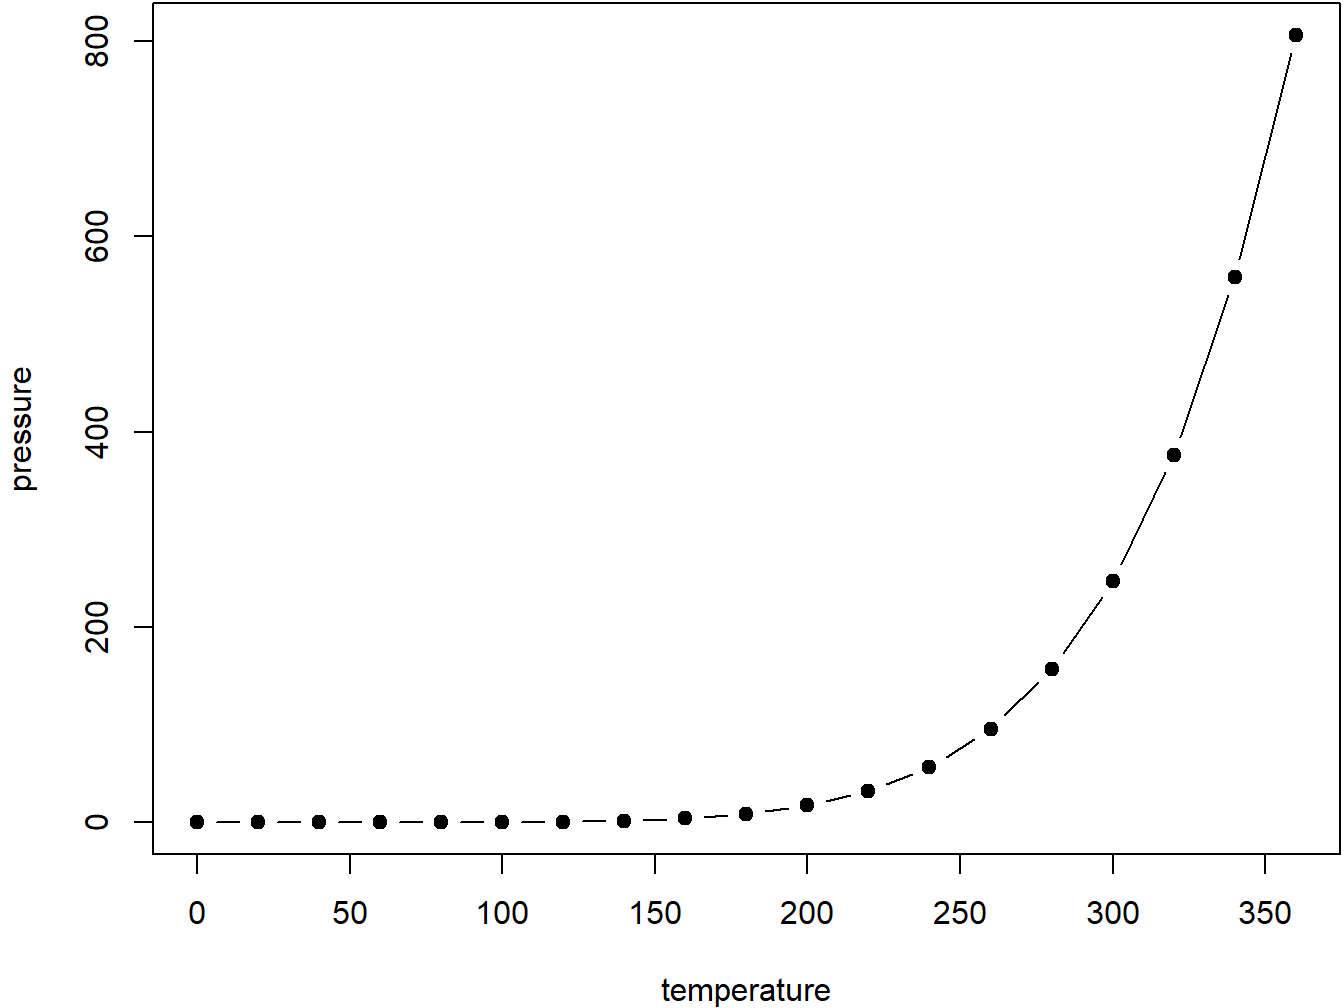
\includegraphics[width=0.8\linewidth]{qpad-book_files/figure-latex/nice-fig-1} 

}

\caption{Here is a nice figure!}\label{fig:nice-fig}
\end{figure}

Reference a figure by its code chunk label with the \texttt{fig:} prefix, e.g., see Figure \ref{fig:nice-fig}. Similarly, you can reference tables generated from \texttt{knitr::kable()}, e.g., see Table \ref{tab:nice-tab}.

\begin{Shaded}
\begin{Highlighting}[]
\NormalTok{knitr}\OperatorTok{::}\KeywordTok{kable}\NormalTok{(}
  \KeywordTok{head}\NormalTok{(iris, }\DecValTok{20}\NormalTok{), }\DataTypeTok{caption =} \StringTok{'Here is a nice table!'}\NormalTok{,}
  \DataTypeTok{booktabs =} \OtherTok{TRUE}
\NormalTok{)}
\end{Highlighting}
\end{Shaded}

\begin{table}[t]

\caption{\label{tab:nice-tab}Here is a nice table!}
\centering
\begin{tabular}{rrrrl}
\toprule
Sepal.Length & Sepal.Width & Petal.Length & Petal.Width & Species\\
\midrule
5.1 & 3.5 & 1.4 & 0.2 & setosa\\
4.9 & 3.0 & 1.4 & 0.2 & setosa\\
4.7 & 3.2 & 1.3 & 0.2 & setosa\\
4.6 & 3.1 & 1.5 & 0.2 & setosa\\
5.0 & 3.6 & 1.4 & 0.2 & setosa\\
\addlinespace
5.4 & 3.9 & 1.7 & 0.4 & setosa\\
4.6 & 3.4 & 1.4 & 0.3 & setosa\\
5.0 & 3.4 & 1.5 & 0.2 & setosa\\
4.4 & 2.9 & 1.4 & 0.2 & setosa\\
4.9 & 3.1 & 1.5 & 0.1 & setosa\\
\addlinespace
5.4 & 3.7 & 1.5 & 0.2 & setosa\\
4.8 & 3.4 & 1.6 & 0.2 & setosa\\
4.8 & 3.0 & 1.4 & 0.1 & setosa\\
4.3 & 3.0 & 1.1 & 0.1 & setosa\\
5.8 & 4.0 & 1.2 & 0.2 & setosa\\
\addlinespace
5.7 & 4.4 & 1.5 & 0.4 & setosa\\
5.4 & 3.9 & 1.3 & 0.4 & setosa\\
5.1 & 3.5 & 1.4 & 0.3 & setosa\\
5.7 & 3.8 & 1.7 & 0.3 & setosa\\
5.1 & 3.8 & 1.5 & 0.3 & setosa\\
\bottomrule
\end{tabular}
\end{table}

You can write citations, too. For example, we are using the \textbf{bookdown} package \citep{R-bookdown} in this sample book, which was built on top of R Markdown and \textbf{knitr} \citep{xie2015}.

\hypertarget{intro}{%
\chapter{Introduction}\label{intro}}

\begin{quote}
All assumptions are violated, but some are more than others
\end{quote}

A comparison of apples and oranges occurs when two items or
groups of items are compared that cannot be practically compared
(\href{https://en.wikipedia.org/wiki/Apples_and_oranges}{Wikipedia}).
The way we measure things can have a big impact on the outcome
of that measurement. For example, you might say that
``I saw 5 robins walking down the road'', while I might say that
``I only saw one robin while sitting on my porch''.
Who say more robins? If looking at only the numeric results,
you saw more robins than me. But this seems like
an apples to oranges comparison.

To compare apples to apples, we need to agree on a comparable
measurement scheme, or at least figure out how does \emph{effort}
affect the observations.

Effort in our example can depend on, e.g.
the \emph{area} of the physical space searched,
the amount of \emph{time} spent, etc.
The outcome might further affected by
weather, time of year, time of day, location,
experience and skill level of the observer.

All these factors can affect the observed count.
Which brings us to the definition of a \emph{point count}:
a trained observer
records all the birds
seen and heard
from a point count station
for a set period of time
within a defined distance radius.

Point count duration and distance have profound effect
on the counts, as shown in Figure \ref{fig:intro-1}
showing that a 10-min unlimited distance count
is roughly 300\% increased compared to 3-min 50-m counts
(averaged across 54 species of boreal songbirds, Matsuoka et al.~2014).

\begin{figure}
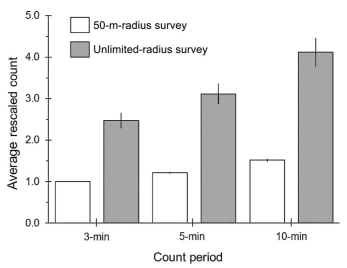
\includegraphics[width=0.8\linewidth]{./images/matsuoka-2014-fig-2} \caption{Effects of duration and distance on mean counts (Matsuoka et al. 2014).}\label{fig:intro-1}
\end{figure}

Point counts are commonly used to answer questions like:

\begin{itemize}
\tightlist
\item
  How many? (Abundance, density, population size)
\item
  Is this location part of the range? (0/1)
\item
  How is abundance changing in space? (Distribution)
\item
  How is abundance changing in time? (Trend)
\item
  What is the effect of a treatment on abundance?
\end{itemize}

\hypertarget{design-based-approaches}{%
\section{Design-based approaches}\label{design-based-approaches}}

Standards and recommendations can
maximize efficiency in the numbers of birds and species counted,
minimize extraneous variability in the counts.

But programs started to deviate from standards:
\emph{``For example, only 3\% of 196,000 point counts conducted during the period
1992--2011 across Alaska and Canada followed the standards recommended for the count period and count radius''} (Matsuoka et al.~2014).
Figure \ref{fig:intro-2} show how point count protocol varies
across the boreal region of North America.

\begin{figure}
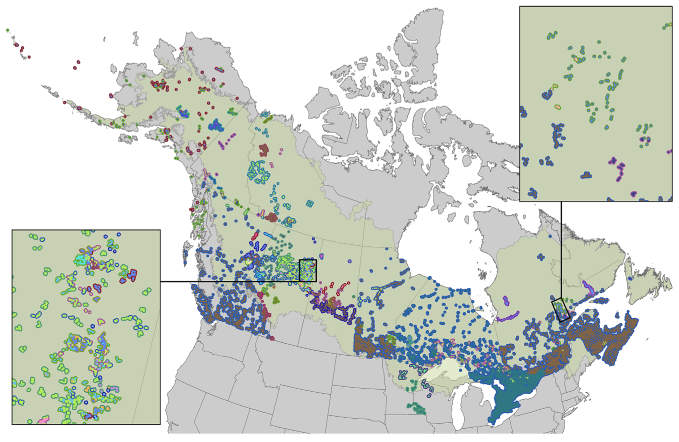
\includegraphics[width=0.8\linewidth]{./images/barker-2015-fig-2} \caption{Survey methodology variation (colors) among contributed projects in the Boreal Avian Modelling (BAM) data base (Barker et al. 2015).}\label{fig:intro-2}
\end{figure}

\BeginKnitrBlock{rmdexercise}
\textbf{Exercise}

In what regard can protocols differ?

What might drive protocol variation among projects?

Why have we abandoned following protocols?
\EndKnitrBlock{rmdexercise}

\hypertarget{model-based-approaches}{%
\section{Model-based approaches}\label{model-based-approaches}}

Detection probabilities might vary even with fixed effort
(we'll cover this more later),
and programs might have their own goals and constraints (access, training, etc).
These constraints would make it almost impossible, and potentially costly
to set up very specific standards.

Labour intensive methods for unmarked populations
have come to the forefront, and computing power of
personal computers opened the door for model-based approaches,
that can accomodate more variation given enough information
in the observed data. These methods often rely on ancillary
information and often some sort of replication.

Some of the commonly used model-based approaches are:

\begin{itemize}
\tightlist
\item
  double observer (\href{https://doi.org/10.1642/0004-8038(2000)117\%5B0393:ADOAFE\%5D2.0.CO;2}{Nichols et al.~2000}),
\item
  distance sampling (\href{https://global.oup.com/academic/product/introduction-to-distance-sampling-9780198509271}{Buckland et al.~2001}),
\item
  removal sampling (\href{https://doi.org/10.1642/0004-8038(2002)119\%5B0414:ARMFED\%5D2.0.CO;2}{Farnsworth et al.~2002}),
\item
  multiple visit occupancy (\href{https://doi.org/10.1890/0012-9658(2002)083\%5B2248:ESORWD\%5D2.0.CO;2}{MacKenzie et al.~2002}),
\item
  multiple visit abundance (\href{https://doi.org/10.1111/j.0006-341X.2004.00142.x}{Royle 2004}).
\end{itemize}

Models come with assumptions, such as:

\begin{itemize}
\tightlist
\item
  population is closed during multiple visits,
\item
  observers are independent,
\item
  all individuals emit cues with identical rates,
\item
  spatial distribution of individuals is uniform,
\item
  etc.
\end{itemize}

Although assumptions are everywhere, we are really good at ignoring
and violating them.

\BeginKnitrBlock{rmdexercise}
\textbf{Exercise}

Can you mention some assumptions from everyday life?

Can you explain why we neglect/violate assumptions in these situations?
\EndKnitrBlock{rmdexercise}

Assumptions are violated, because we seek simplicity.
The main question we have to ask: \emph{does it matter in practice} if
we violate the assumptions?

\hypertarget{our-approach}{%
\section{Our approach}\label{our-approach}}

In this book and course, we will critically evaluate common assumptions made
when analyzing point count data using the following approach:

\begin{enumerate}
\def\labelenumi{\arabic{enumi}.}
\tightlist
\item
  we will introduce a concept,
\item
  understand how we can infer it from data,
\item
  then we recreate the situation \emph{in silico},
\item
  and see how the outcome changes as we make different assumptions.
\end{enumerate}

It is guaranteed that we will violate every assumption we make.
To get away with it, we need to understand how much is too much,
and whether it has an impact in practice.
If there is a practical consequence, we will look at ways to minimize
that effects -- so that we can safely ignore the assumption.

\hypertarget{r-basics}{%
\section{R basics}\label{r-basics}}

This short document is intended to help you brush up your R skills.
If you feel that these R basics are not very familiar,
I suggest to take a look at some introductory R books,
sich as this preprint version of Norman Matloff's \emph{The Art of R Programming} book: \url{http://heather.cs.ucdavis.edu/~matloff/132/NSPpart.pdf}, check out Chapters 1--6.

R is a great calculator:

\begin{Shaded}
\begin{Highlighting}[]
\DecValTok{1} \OperatorTok{+}\StringTok{ }\DecValTok{2}
\end{Highlighting}
\end{Shaded}

\begin{verbatim}
## [1] 3
\end{verbatim}

Assign a value and print an object using \texttt{=} or \texttt{\textless{}-} (preferred in this book):

\begin{Shaded}
\begin{Highlighting}[]
\NormalTok{(}\DataTypeTok{x =} \DecValTok{2}\NormalTok{) }\CommentTok{# shorthand for print}
\end{Highlighting}
\end{Shaded}

\begin{verbatim}
## [1] 2
\end{verbatim}

\begin{Shaded}
\begin{Highlighting}[]
\KeywordTok{print}\NormalTok{(x)}
\end{Highlighting}
\end{Shaded}

\begin{verbatim}
## [1] 2
\end{verbatim}

\begin{Shaded}
\begin{Highlighting}[]
\NormalTok{x }\OperatorTok{==}\StringTok{ }\DecValTok{2} \CommentTok{# logical operator, not assignment}
\end{Highlighting}
\end{Shaded}

\begin{verbatim}
## [1] TRUE
\end{verbatim}

\begin{Shaded}
\begin{Highlighting}[]
\NormalTok{y <-}\StringTok{ }\NormalTok{x }\OperatorTok{+}\StringTok{ }\FloatTok{0.5}
\NormalTok{y }\CommentTok{# another way to print}
\end{Highlighting}
\end{Shaded}

\begin{verbatim}
## [1] 2.5
\end{verbatim}

Logical operators come handy:

\begin{Shaded}
\begin{Highlighting}[]
\NormalTok{x }\OperatorTok{==}\StringTok{ }\NormalTok{y }\CommentTok{# equal}
\end{Highlighting}
\end{Shaded}

\begin{verbatim}
## [1] FALSE
\end{verbatim}

\begin{Shaded}
\begin{Highlighting}[]
\NormalTok{x }\OperatorTok{!=}\StringTok{ }\NormalTok{y }\CommentTok{# not eaqual}
\end{Highlighting}
\end{Shaded}

\begin{verbatim}
## [1] TRUE
\end{verbatim}

\begin{Shaded}
\begin{Highlighting}[]
\NormalTok{x }\OperatorTok{<}\StringTok{ }\NormalTok{y }\CommentTok{# smaller than}
\end{Highlighting}
\end{Shaded}

\begin{verbatim}
## [1] TRUE
\end{verbatim}

\begin{Shaded}
\begin{Highlighting}[]
\NormalTok{x }\OperatorTok{>=}\StringTok{ }\NormalTok{y }\CommentTok{# greater than or equal}
\end{Highlighting}
\end{Shaded}

\begin{verbatim}
## [1] FALSE
\end{verbatim}

Vectors and sequences are created most often by the functions
\texttt{c}, \texttt{:}, \texttt{seq}, and \texttt{rep}:

\begin{Shaded}
\begin{Highlighting}[]
\NormalTok{x <-}\StringTok{ }\KeywordTok{c}\NormalTok{(}\DecValTok{1}\NormalTok{, }\DecValTok{2}\NormalTok{, }\DecValTok{3}\NormalTok{)}
\NormalTok{x}
\end{Highlighting}
\end{Shaded}

\begin{verbatim}
## [1] 1 2 3
\end{verbatim}

\begin{Shaded}
\begin{Highlighting}[]
\DecValTok{1}\OperatorTok{:}\DecValTok{3}
\end{Highlighting}
\end{Shaded}

\begin{verbatim}
## [1] 1 2 3
\end{verbatim}

\begin{Shaded}
\begin{Highlighting}[]
\KeywordTok{seq}\NormalTok{(}\DecValTok{1}\NormalTok{, }\DecValTok{3}\NormalTok{, }\DataTypeTok{by =} \DecValTok{1}\NormalTok{)}
\end{Highlighting}
\end{Shaded}

\begin{verbatim}
## [1] 1 2 3
\end{verbatim}

\begin{Shaded}
\begin{Highlighting}[]
\KeywordTok{rep}\NormalTok{(}\DecValTok{1}\NormalTok{, }\DecValTok{5}\NormalTok{)}
\end{Highlighting}
\end{Shaded}

\begin{verbatim}
## [1] 1 1 1 1 1
\end{verbatim}

\begin{Shaded}
\begin{Highlighting}[]
\KeywordTok{rep}\NormalTok{(}\DecValTok{1}\OperatorTok{:}\DecValTok{2}\NormalTok{, }\DecValTok{5}\NormalTok{)}
\end{Highlighting}
\end{Shaded}

\begin{verbatim}
##  [1] 1 2 1 2 1 2 1 2 1 2
\end{verbatim}

\begin{Shaded}
\begin{Highlighting}[]
\KeywordTok{rep}\NormalTok{(}\DecValTok{1}\OperatorTok{:}\DecValTok{2}\NormalTok{, }\DataTypeTok{each =} \DecValTok{5}\NormalTok{)}
\end{Highlighting}
\end{Shaded}

\begin{verbatim}
##  [1] 1 1 1 1 1 2 2 2 2 2
\end{verbatim}

When doing operations with vectors remember that values of
the shorter object are recycled:

\begin{Shaded}
\begin{Highlighting}[]
\NormalTok{x }\OperatorTok{+}\StringTok{ }\FloatTok{0.5}
\end{Highlighting}
\end{Shaded}

\begin{verbatim}
## [1] 1.5 2.5 3.5
\end{verbatim}

\begin{Shaded}
\begin{Highlighting}[]
\NormalTok{x }\OperatorTok{*}\StringTok{ }\KeywordTok{c}\NormalTok{(}\DecValTok{10}\NormalTok{, }\DecValTok{11}\NormalTok{, }\DecValTok{12}\NormalTok{, }\DecValTok{13}\NormalTok{)}
\end{Highlighting}
\end{Shaded}

\begin{verbatim}
## Warning in x * c(10, 11, 12, 13): longer object length is not a
## multiple of shorter object length
\end{verbatim}

\begin{verbatim}
## [1] 10 22 36 13
\end{verbatim}

Indexing and ordering vectors is a a fundamental skill:

\begin{Shaded}
\begin{Highlighting}[]
\NormalTok{x[}\DecValTok{1}\NormalTok{]}
\end{Highlighting}
\end{Shaded}

\begin{verbatim}
## [1] 1
\end{verbatim}

\begin{Shaded}
\begin{Highlighting}[]
\NormalTok{x[}\KeywordTok{c}\NormalTok{(}\DecValTok{1}\NormalTok{, }\DecValTok{1}\NormalTok{, }\DecValTok{1}\NormalTok{)] }\CommentTok{# a way of repeatig values}
\end{Highlighting}
\end{Shaded}

\begin{verbatim}
## [1] 1 1 1
\end{verbatim}

\begin{Shaded}
\begin{Highlighting}[]
\NormalTok{x[}\DecValTok{1}\OperatorTok{:}\DecValTok{2}\NormalTok{]}
\end{Highlighting}
\end{Shaded}

\begin{verbatim}
## [1] 1 2
\end{verbatim}

\begin{Shaded}
\begin{Highlighting}[]
\NormalTok{x[x }\OperatorTok{!=}\StringTok{ }\DecValTok{2}\NormalTok{]}
\end{Highlighting}
\end{Shaded}

\begin{verbatim}
## [1] 1 3
\end{verbatim}

\begin{Shaded}
\begin{Highlighting}[]
\NormalTok{x[x }\OperatorTok{==}\StringTok{ }\DecValTok{2}\NormalTok{]}
\end{Highlighting}
\end{Shaded}

\begin{verbatim}
## [1] 2
\end{verbatim}

\begin{Shaded}
\begin{Highlighting}[]
\NormalTok{x[x }\OperatorTok{>}\StringTok{ }\DecValTok{1} \OperatorTok{&}\StringTok{ }\NormalTok{x }\OperatorTok{<}\StringTok{ }\DecValTok{3}\NormalTok{]}
\end{Highlighting}
\end{Shaded}

\begin{verbatim}
## [1] 2
\end{verbatim}

\begin{Shaded}
\begin{Highlighting}[]
\KeywordTok{order}\NormalTok{(x, }\DataTypeTok{decreasing=}\OtherTok{TRUE}\NormalTok{)}
\end{Highlighting}
\end{Shaded}

\begin{verbatim}
## [1] 3 2 1
\end{verbatim}

\begin{Shaded}
\begin{Highlighting}[]
\NormalTok{x[}\KeywordTok{order}\NormalTok{(x, }\DataTypeTok{decreasing=}\OtherTok{TRUE}\NormalTok{)]}
\end{Highlighting}
\end{Shaded}

\begin{verbatim}
## [1] 3 2 1
\end{verbatim}

\begin{Shaded}
\begin{Highlighting}[]
\KeywordTok{rev}\NormalTok{(x) }\CommentTok{# reverse}
\end{Highlighting}
\end{Shaded}

\begin{verbatim}
## [1] 3 2 1
\end{verbatim}

See how \texttt{NA} values can influence
sorting character vectors:

\begin{Shaded}
\begin{Highlighting}[]
\NormalTok{z <-}\StringTok{ }\KeywordTok{c}\NormalTok{(}\StringTok{"b"}\NormalTok{, }\StringTok{"a"}\NormalTok{, }\StringTok{"c"}\NormalTok{, }\OtherTok{NA}\NormalTok{)}
\NormalTok{z[z }\OperatorTok{==}\StringTok{ "a"}\NormalTok{]}
\end{Highlighting}
\end{Shaded}

\begin{verbatim}
## [1] "a" NA
\end{verbatim}

\begin{Shaded}
\begin{Highlighting}[]
\NormalTok{z[}\OperatorTok{!}\KeywordTok{is.na}\NormalTok{(z) }\OperatorTok{&}\StringTok{ }\NormalTok{z }\OperatorTok{==}\StringTok{ "a"}\NormalTok{]}
\end{Highlighting}
\end{Shaded}

\begin{verbatim}
## [1] "a"
\end{verbatim}

\begin{Shaded}
\begin{Highlighting}[]
\NormalTok{z[}\KeywordTok{is.na}\NormalTok{(z) }\OperatorTok{|}\StringTok{ }\NormalTok{z }\OperatorTok{==}\StringTok{ "a"}\NormalTok{]}
\end{Highlighting}
\end{Shaded}

\begin{verbatim}
## [1] "a" NA
\end{verbatim}

\begin{Shaded}
\begin{Highlighting}[]
\KeywordTok{is.na}\NormalTok{(z)}
\end{Highlighting}
\end{Shaded}

\begin{verbatim}
## [1] FALSE FALSE FALSE  TRUE
\end{verbatim}

\begin{Shaded}
\begin{Highlighting}[]
\KeywordTok{which}\NormalTok{(}\KeywordTok{is.na}\NormalTok{(z))}
\end{Highlighting}
\end{Shaded}

\begin{verbatim}
## [1] 4
\end{verbatim}

\begin{Shaded}
\begin{Highlighting}[]
\KeywordTok{sort}\NormalTok{(z)}
\end{Highlighting}
\end{Shaded}

\begin{verbatim}
## [1] "a" "b" "c"
\end{verbatim}

\begin{Shaded}
\begin{Highlighting}[]
\KeywordTok{sort}\NormalTok{(z, }\DataTypeTok{na.last=}\OtherTok{TRUE}\NormalTok{)}
\end{Highlighting}
\end{Shaded}

\begin{verbatim}
## [1] "a" "b" "c" NA
\end{verbatim}

There are a few special values:

\begin{Shaded}
\begin{Highlighting}[]
\KeywordTok{as.numeric}\NormalTok{(}\KeywordTok{c}\NormalTok{(}\StringTok{"1"}\NormalTok{, }\StringTok{"a"}\NormalTok{)) }\CommentTok{# NA: not available (missing or invalid)}
\end{Highlighting}
\end{Shaded}

\begin{verbatim}
## Warning: NAs introduced by coercion
\end{verbatim}

\begin{verbatim}
## [1]  1 NA
\end{verbatim}

\begin{Shaded}
\begin{Highlighting}[]
\DecValTok{0}\OperatorTok{/}\DecValTok{0} \CommentTok{# NaN: not a number}
\end{Highlighting}
\end{Shaded}

\begin{verbatim}
## [1] NaN
\end{verbatim}

\begin{Shaded}
\begin{Highlighting}[]
\DecValTok{1}\OperatorTok{/}\DecValTok{0} \CommentTok{# Inf}
\end{Highlighting}
\end{Shaded}

\begin{verbatim}
## [1] Inf
\end{verbatim}

\begin{Shaded}
\begin{Highlighting}[]
\DecValTok{-1}\OperatorTok{/}\DecValTok{0} \CommentTok{# -Inf}
\end{Highlighting}
\end{Shaded}

\begin{verbatim}
## [1] -Inf
\end{verbatim}

Matrices and arrays are vectors with dimensions, elements are in same mode:

\begin{Shaded}
\begin{Highlighting}[]
\NormalTok{(m <-}\StringTok{ }\KeywordTok{matrix}\NormalTok{(}\DecValTok{1}\OperatorTok{:}\DecValTok{12}\NormalTok{, }\DecValTok{4}\NormalTok{, }\DecValTok{3}\NormalTok{))}
\end{Highlighting}
\end{Shaded}

\begin{verbatim}
##      [,1] [,2] [,3]
## [1,]    1    5    9
## [2,]    2    6   10
## [3,]    3    7   11
## [4,]    4    8   12
\end{verbatim}

\begin{Shaded}
\begin{Highlighting}[]
\KeywordTok{matrix}\NormalTok{(}\DecValTok{1}\OperatorTok{:}\DecValTok{12}\NormalTok{, }\DecValTok{4}\NormalTok{, }\DecValTok{3}\NormalTok{, }\DataTypeTok{byrow=}\OtherTok{TRUE}\NormalTok{)}
\end{Highlighting}
\end{Shaded}

\begin{verbatim}
##      [,1] [,2] [,3]
## [1,]    1    2    3
## [2,]    4    5    6
## [3,]    7    8    9
## [4,]   10   11   12
\end{verbatim}

\begin{Shaded}
\begin{Highlighting}[]
\KeywordTok{array}\NormalTok{(}\DecValTok{1}\OperatorTok{:}\DecValTok{12}\NormalTok{, }\KeywordTok{c}\NormalTok{(}\DecValTok{2}\NormalTok{, }\DecValTok{2}\NormalTok{, }\DecValTok{3}\NormalTok{))}
\end{Highlighting}
\end{Shaded}

\begin{verbatim}
## , , 1
## 
##      [,1] [,2]
## [1,]    1    3
## [2,]    2    4
## 
## , , 2
## 
##      [,1] [,2]
## [1,]    5    7
## [2,]    6    8
## 
## , , 3
## 
##      [,1] [,2]
## [1,]    9   11
## [2,]   10   12
\end{verbatim}

Many objects have attributes:

\begin{Shaded}
\begin{Highlighting}[]
\KeywordTok{dim}\NormalTok{(m)}
\end{Highlighting}
\end{Shaded}

\begin{verbatim}
## [1] 4 3
\end{verbatim}

\begin{Shaded}
\begin{Highlighting}[]
\KeywordTok{dim}\NormalTok{(m) <-}\StringTok{ }\OtherTok{NULL}
\NormalTok{m}
\end{Highlighting}
\end{Shaded}

\begin{verbatim}
##  [1]  1  2  3  4  5  6  7  8  9 10 11 12
\end{verbatim}

\begin{Shaded}
\begin{Highlighting}[]
\KeywordTok{dim}\NormalTok{(m) <-}\StringTok{ }\KeywordTok{c}\NormalTok{(}\DecValTok{4}\NormalTok{, }\DecValTok{3}\NormalTok{)}
\NormalTok{m}
\end{Highlighting}
\end{Shaded}

\begin{verbatim}
##      [,1] [,2] [,3]
## [1,]    1    5    9
## [2,]    2    6   10
## [3,]    3    7   11
## [4,]    4    8   12
\end{verbatim}

\begin{Shaded}
\begin{Highlighting}[]
\KeywordTok{dimnames}\NormalTok{(m) <-}\StringTok{ }\KeywordTok{list}\NormalTok{(letters[}\DecValTok{1}\OperatorTok{:}\DecValTok{4}\NormalTok{], LETTERS[}\DecValTok{1}\OperatorTok{:}\DecValTok{3}\NormalTok{])}
\NormalTok{m}
\end{Highlighting}
\end{Shaded}

\begin{verbatim}
##   A B  C
## a 1 5  9
## b 2 6 10
## c 3 7 11
## d 4 8 12
\end{verbatim}

\begin{Shaded}
\begin{Highlighting}[]
\KeywordTok{attributes}\NormalTok{(m)}
\end{Highlighting}
\end{Shaded}

\begin{verbatim}
## $dim
## [1] 4 3
## 
## $dimnames
## $dimnames[[1]]
## [1] "a" "b" "c" "d"
## 
## $dimnames[[2]]
## [1] "A" "B" "C"
\end{verbatim}

Matrice and indices:

\begin{Shaded}
\begin{Highlighting}[]
\NormalTok{m[}\DecValTok{1}\OperatorTok{:}\DecValTok{2}\NormalTok{,]}
\end{Highlighting}
\end{Shaded}

\begin{verbatim}
##   A B  C
## a 1 5  9
## b 2 6 10
\end{verbatim}

\begin{Shaded}
\begin{Highlighting}[]
\NormalTok{m[}\DecValTok{1}\NormalTok{,}\DecValTok{2}\NormalTok{]}
\end{Highlighting}
\end{Shaded}

\begin{verbatim}
## [1] 5
\end{verbatim}

\begin{Shaded}
\begin{Highlighting}[]
\NormalTok{m[,}\DecValTok{2}\NormalTok{]}
\end{Highlighting}
\end{Shaded}

\begin{verbatim}
## a b c d 
## 5 6 7 8
\end{verbatim}

\begin{Shaded}
\begin{Highlighting}[]
\NormalTok{m[,}\DecValTok{2}\NormalTok{,drop=}\OtherTok{FALSE}\NormalTok{]}
\end{Highlighting}
\end{Shaded}

\begin{verbatim}
##   B
## a 5
## b 6
## c 7
## d 8
\end{verbatim}

\begin{Shaded}
\begin{Highlighting}[]
\NormalTok{m[}\DecValTok{2}\NormalTok{]}
\end{Highlighting}
\end{Shaded}

\begin{verbatim}
## [1] 2
\end{verbatim}

\begin{Shaded}
\begin{Highlighting}[]
\NormalTok{m[}\KeywordTok{rownames}\NormalTok{(m) }\OperatorTok{==}\StringTok{ "c"}\NormalTok{,]}
\end{Highlighting}
\end{Shaded}

\begin{verbatim}
##  A  B  C 
##  3  7 11
\end{verbatim}

\begin{Shaded}
\begin{Highlighting}[]
\NormalTok{m[}\KeywordTok{rownames}\NormalTok{(m) }\OperatorTok{!=}\StringTok{ "c"}\NormalTok{,]}
\end{Highlighting}
\end{Shaded}

\begin{verbatim}
##   A B  C
## a 1 5  9
## b 2 6 10
## d 4 8 12
\end{verbatim}

\begin{Shaded}
\begin{Highlighting}[]
\NormalTok{m[}\KeywordTok{rownames}\NormalTok{(m) }\OperatorTok\StringTok{ }\KeywordTok{c}\NormalTok{(}\StringTok{"a"}\NormalTok{, }\StringTok{"c"}\NormalTok{, }\StringTok{"e"}\NormalTok{),]}
\end{Highlighting}
\end{Shaded}

\begin{verbatim}
##   A B  C
## a 1 5  9
## c 3 7 11
\end{verbatim}

\begin{Shaded}
\begin{Highlighting}[]
\NormalTok{m[}\OperatorTok{!}\NormalTok{(}\KeywordTok{rownames}\NormalTok{(m) }\OperatorTok\StringTok{ }\KeywordTok{c}\NormalTok{(}\StringTok{"a"}\NormalTok{, }\StringTok{"c"}\NormalTok{, }\StringTok{"e"}\NormalTok{)),]}
\end{Highlighting}
\end{Shaded}

\begin{verbatim}
##   A B  C
## b 2 6 10
## d 4 8 12
\end{verbatim}

Lists and indexing:

\begin{Shaded}
\begin{Highlighting}[]
\NormalTok{l <-}\StringTok{ }\KeywordTok{list}\NormalTok{(}\DataTypeTok{m =}\NormalTok{ m, }\DataTypeTok{x =}\NormalTok{ x, }\DataTypeTok{z =}\NormalTok{ z)}
\NormalTok{l}
\end{Highlighting}
\end{Shaded}

\begin{verbatim}
## $m
##   A B  C
## a 1 5  9
## b 2 6 10
## c 3 7 11
## d 4 8 12
## 
## $x
## [1] 1 2 3
## 
## $z
## [1] "b" "a" "c" NA
\end{verbatim}

\begin{Shaded}
\begin{Highlighting}[]
\NormalTok{l}\OperatorTok{$}\NormalTok{ddd <-}\StringTok{ }\KeywordTok{sqrt}\NormalTok{(l}\OperatorTok{$}\NormalTok{x)}
\NormalTok{l[}\DecValTok{2}\OperatorTok{:}\DecValTok{3}\NormalTok{]}
\end{Highlighting}
\end{Shaded}

\begin{verbatim}
## $x
## [1] 1 2 3
## 
## $z
## [1] "b" "a" "c" NA
\end{verbatim}

\begin{Shaded}
\begin{Highlighting}[]
\NormalTok{l[[}\StringTok{"ddd"}\NormalTok{]]}
\end{Highlighting}
\end{Shaded}

\begin{verbatim}
## [1] 1.000 1.414 1.732
\end{verbatim}

Data frames are often required for statistical modeling.
A data frame is a list where length of elements match and elements
can be in different mode.

\begin{Shaded}
\begin{Highlighting}[]
\NormalTok{d <-}\StringTok{ }\KeywordTok{data.frame}\NormalTok{(}\DataTypeTok{x =}\NormalTok{ x, }\DataTypeTok{sqrt_x =} \KeywordTok{sqrt}\NormalTok{(x))}
\NormalTok{d}
\end{Highlighting}
\end{Shaded}

Inspect structure of R objects:

\begin{Shaded}
\begin{Highlighting}[]
\KeywordTok{str}\NormalTok{(x)}
\end{Highlighting}
\end{Shaded}

\begin{verbatim}
##  num [1:3] 1 2 3
\end{verbatim}

\begin{Shaded}
\begin{Highlighting}[]
\KeywordTok{str}\NormalTok{(z)}
\end{Highlighting}
\end{Shaded}

\begin{verbatim}
##  chr [1:4] "b" "a" "c" NA
\end{verbatim}

\begin{Shaded}
\begin{Highlighting}[]
\KeywordTok{str}\NormalTok{(m)}
\end{Highlighting}
\end{Shaded}

\begin{verbatim}
##  int [1:4, 1:3] 1 2 3 4 5 6 7 8 9 10 ...
##  - attr(*, "dimnames")=List of 2
##   ..$ : chr [1:4] "a" "b" "c" "d"
##   ..$ : chr [1:3] "A" "B" "C"
\end{verbatim}

\begin{Shaded}
\begin{Highlighting}[]
\KeywordTok{str}\NormalTok{(l)}
\end{Highlighting}
\end{Shaded}

\begin{verbatim}
## List of 4
##  $ m  : int [1:4, 1:3] 1 2 3 4 5 6 7 8 9 10 ...
##   ..- attr(*, "dimnames")=List of 2
##   .. ..$ : chr [1:4] "a" "b" "c" "d"
##   .. ..$ : chr [1:3] "A" "B" "C"
##  $ x  : num [1:3] 1 2 3
##  $ z  : chr [1:4] "b" "a" "c" NA
##  $ ddd: num [1:3] 1 1.41 1.73
\end{verbatim}

\begin{Shaded}
\begin{Highlighting}[]
\KeywordTok{str}\NormalTok{(d)}
\end{Highlighting}
\end{Shaded}

\begin{verbatim}
## 'data.frame':    3 obs. of  2 variables:
##  $ x     : num  1 2 3
##  $ sqrt_x: num  1 1.41 1.73
\end{verbatim}

\begin{Shaded}
\begin{Highlighting}[]
\KeywordTok{str}\NormalTok{(}\KeywordTok{as.data.frame}\NormalTok{(m))}
\end{Highlighting}
\end{Shaded}

\begin{verbatim}
## 'data.frame':    4 obs. of  3 variables:
##  $ A: int  1 2 3 4
##  $ B: int  5 6 7 8
##  $ C: int  9 10 11 12
\end{verbatim}

\begin{Shaded}
\begin{Highlighting}[]
\KeywordTok{str}\NormalTok{(}\KeywordTok{as.list}\NormalTok{(d))}
\end{Highlighting}
\end{Shaded}

\begin{verbatim}
## List of 2
##  $ x     : num [1:3] 1 2 3
##  $ sqrt_x: num [1:3] 1 1.41 1.73
\end{verbatim}

Get summaries of these objects:

\begin{Shaded}
\begin{Highlighting}[]
\KeywordTok{summary}\NormalTok{(x)}
\end{Highlighting}
\end{Shaded}

\begin{verbatim}
##    Min. 1st Qu.  Median    Mean 3rd Qu.    Max. 
##     1.0     1.5     2.0     2.0     2.5     3.0
\end{verbatim}

\begin{Shaded}
\begin{Highlighting}[]
\KeywordTok{summary}\NormalTok{(z)}
\end{Highlighting}
\end{Shaded}

\begin{verbatim}
##    Length     Class      Mode 
##         4 character character
\end{verbatim}

\begin{Shaded}
\begin{Highlighting}[]
\KeywordTok{summary}\NormalTok{(m)}
\end{Highlighting}
\end{Shaded}

\begin{verbatim}
##        A              B              C        
##  Min.   :1.00   Min.   :5.00   Min.   : 9.00  
##  1st Qu.:1.75   1st Qu.:5.75   1st Qu.: 9.75  
##  Median :2.50   Median :6.50   Median :10.50  
##  Mean   :2.50   Mean   :6.50   Mean   :10.50  
##  3rd Qu.:3.25   3rd Qu.:7.25   3rd Qu.:11.25  
##  Max.   :4.00   Max.   :8.00   Max.   :12.00
\end{verbatim}

\begin{Shaded}
\begin{Highlighting}[]
\KeywordTok{summary}\NormalTok{(l)}
\end{Highlighting}
\end{Shaded}

\begin{verbatim}
##     Length Class  Mode     
## m   12     -none- numeric  
## x    3     -none- numeric  
## z    4     -none- character
## ddd  3     -none- numeric
\end{verbatim}

\begin{Shaded}
\begin{Highlighting}[]
\KeywordTok{summary}\NormalTok{(d)}
\end{Highlighting}
\end{Shaded}

\begin{verbatim}
##        x           sqrt_x    
##  Min.   :1.0   Min.   :1.00  
##  1st Qu.:1.5   1st Qu.:1.21  
##  Median :2.0   Median :1.41  
##  Mean   :2.0   Mean   :1.38  
##  3rd Qu.:2.5   3rd Qu.:1.57  
##  Max.   :3.0   Max.   :1.73
\end{verbatim}

\hypertarget{pcdata}{%
\chapter{Organizing and Processing Point Count Data}\label{pcdata}}

\begin{quote}
All data are messy, but some are missing
\end{quote}

It is often called \emph{data processing}, \emph{data munging},
\emph{data wrangling}, \emph{data cleaning}.
None of these expressions capture the dread associated with the actual activity.

Luckily, there are only 4 things that can get messed up:

\begin{enumerate}
\def\labelenumi{\arabic{enumi}.}
\tightlist
\item
  space (e.g.~wrong UTM zones),
\item
  time (ISO format please),
\item
  taxonomy (UNK, mis-ID),
\item
  something else (if there were no errors, check again).
\end{enumerate}

\hypertarget{josm-data-set}{%
\section{JOSM data set}\label{josm-data-set}}

Look at the source code in the \texttt{\_data/josm} directory of the book
if you are interested in data processing details.
We skip that for now.

\includegraphics[width=13.89in]{./images/mahon-2016-fig-1}

Cause-Effect Monitoring Migratory Landbirds at Regional Scales:
understand how boreal songbirds are affected by human activity in the oil sands area.

\includegraphics[width=13.89in]{./images/mahon-2016-fig-2}

Survey area boundary (\(r\)=2.5 km circle), habitat type and human footprint mapping,
and clustered point count site locations.

Surveys were spatially replicated because:

\begin{itemize}
\tightlist
\item
  we want to make inferences about a population,
\item
  full census is out of reach,
\item
  thus we take a sample of the population
\item
  that is representative and random.
\item
  Ideally, sample size should be as large as possible,
\item
  it reduces variability and
\item
  increases statistical power.
\end{itemize}

Survey locations were pucked based on various criteria:

\begin{itemize}
\tightlist
\item
  stratification (land cover),
\item
  gradients (disturbance levels),
\item
  random location (control for unmeasured effects),
\item
  take into account historical surveys (avoid, or revisit),
\item
  access, cost (clusters).
\end{itemize}

The \texttt{josm} obejct is a list with 3 elements:

\begin{itemize}
\tightlist
\item
  \texttt{surveys}: data frame with survey specific information,
\item
  \texttt{species}: lookup table for species,
\item
  \texttt{counts}: individual counts by survey and species.
\end{itemize}

\begin{Shaded}
\begin{Highlighting}[]
\KeywordTok{library}\NormalTok{(mefa4)}
\KeywordTok{load}\NormalTok{(}\StringTok{"./_data/josm/josm.rda"}\NormalTok{)}
\KeywordTok{names}\NormalTok{(josm)}
\end{Highlighting}
\end{Shaded}

\begin{verbatim}
## [1] "surveys" "species" "counts"
\end{verbatim}

Species info: species codes, common and scientific names. The table could also contain
taxonomic, trait, etc. information as well.

\begin{Shaded}
\begin{Highlighting}[]
\KeywordTok{head}\NormalTok{(josm}\OperatorTok{$}\NormalTok{species)}
\end{Highlighting}
\end{Shaded}

At the survey level, we have coordinates, date/time info,
variables capturing survey conditions, and land cover info extracted from 1 km\(^2\) resolution rasters.

\begin{Shaded}
\begin{Highlighting}[]
\KeywordTok{colnames}\NormalTok{(josm}\OperatorTok{$}\NormalTok{surveys)}
\end{Highlighting}
\end{Shaded}

\begin{verbatim}
##  [1] "SiteID"        "SurveyArea"    "Longitude"    
##  [4] "Latitude"      "Date"          "StationID"    
##  [7] "ObserverID"    "TimeStart"     "VisitID"      
## [10] "WindStart"     "PrecipStart"   "TempStart"    
## [13] "CloudStart"    "WindEnd"       "PrecipEnd"    
## [16] "TempEnd"       "CloudEnd"      "TimeFin"      
## [19] "Noise"         "OvernightRain" "DateTime"     
## [22] "SunRiseTime"   "SunRiseFrac"   "TSSR"         
## [25] "OrdinalDay"    "DAY"           "Open"         
## [28] "Water"         "Agr"           "UrbInd"       
## [31] "SoftLin"       "Roads"         "Decid"        
## [34] "OpenWet"       "Conif"         "ConifWet"
\end{verbatim}

The count table contains one row for each unique individual
of a species (\texttt{SpeciesID} links to the species lookup table)
observed during a survey (\texttt{StationID} links to the survey attribute table).
Check the data dictionary in \texttt{\_data/josm} folder for a detailed explanation of each column.

\begin{Shaded}
\begin{Highlighting}[]
\KeywordTok{str}\NormalTok{(josm}\OperatorTok{$}\NormalTok{counts)}
\end{Highlighting}
\end{Shaded}

\begin{verbatim}
## 'data.frame':    52372 obs. of  18 variables:
##  $ ObservationID: Factor w/ 57024 levels "CL10102-130622-001",..: 1 2 3 4 5 6 8 9 10 11 ...
##  $ SiteID       : Factor w/ 4569 levels "CL10102","CL10106",..: 1 1 1 1 1 1 1 1 2 2 ...
##  $ StationID    : Factor w/ 4569 levels "CL10102-1","CL10106-1",..: 1 1 1 1 1 1 1 1 2 2 ...
##  $ TimeInterval : int  1 1 1 1 5 5 1 1 1 1 ...
##  $ Direction    : int  1 2 2 2 1 4 4 4 1 1 ...
##  $ Distance     : int  1 2 2 1 3 3 2 1 1 1 ...
##  $ DetectType1  : Factor w/ 3 levels "C","S","V": 2 2 2 2 1 1 2 2 2 2 ...
##  $ DetectType2  : Factor w/ 3 levels "C","S","V": NA NA NA NA NA NA NA NA NA NA ...
##  $ DetectType3  : Factor w/ 3 levels "C","S","V": NA NA NA NA NA NA NA NA NA NA ...
##  $ Sex          : Factor w/ 4 levels "F","M","P","U": 2 2 2 2 4 4 2 2 2 2 ...
##  $ Age          : Factor w/ 6 levels "A","F","J","JUV",..: 1 1 1 1 1 1 1 1 1 1 ...
##  $ Activity1    : Factor w/ 17 levels "BE","CF","CH",..: 5 5 5 5 NA NA NA 5 5 NA ...
##  $ Activity2    : Factor w/ 17 levels "48","BE","CF",..: NA NA NA NA NA NA NA NA NA NA ...
##  $ Activity3    : Factor w/ 7 levels "CF","DC","DR",..: NA NA NA NA NA NA NA NA NA NA ...
##  $ ActivityNote : Factor w/ 959 levels "AGITATED","AGITATED CALLING",..: NA NA NA NA NA NA NA NA NA NA ...
##  $ Dur          : Factor w/ 3 levels "0-3min","3-5min",..: 1 1 1 1 3 3 1 1 1 1 ...
##  $ Dis          : Factor w/ 3 levels "0-50m","50-100m",..: 1 2 2 1 3 3 2 1 1 1 ...
##  $ SpeciesID    : Factor w/ 150 levels "ALFL","AMBI",..: 107 95 95 107 46 43 140 95 125 38 ...
\end{verbatim}

\hypertarget{cross-tabulating-species-counts}{%
\section{Cross tabulating species counts}\label{cross-tabulating-species-counts}}

Take the following dummy data frame (long format):

\begin{Shaded}
\begin{Highlighting}[]
\NormalTok{(d <-}\StringTok{ }\KeywordTok{data.frame}\NormalTok{(}
  \DataTypeTok{sample=}\KeywordTok{factor}\NormalTok{(}\KeywordTok{paste0}\NormalTok{(}\StringTok{"S"}\NormalTok{, }\KeywordTok{c}\NormalTok{(}\DecValTok{1}\NormalTok{,}\DecValTok{1}\NormalTok{,}\DecValTok{1}\NormalTok{,}\DecValTok{2}\NormalTok{,}\DecValTok{2}\NormalTok{)), }\KeywordTok{paste0}\NormalTok{(}\StringTok{"S"}\NormalTok{, }\DecValTok{1}\OperatorTok{:}\DecValTok{3}\NormalTok{)),}
  \DataTypeTok{species=}\KeywordTok{c}\NormalTok{(}\StringTok{"BTNW"}\NormalTok{, }\StringTok{"OVEN"}\NormalTok{, }\StringTok{"CANG"}\NormalTok{, }\StringTok{"AMRO"}\NormalTok{, }\StringTok{"CANG"}\NormalTok{),}
  \DataTypeTok{abundance=}\KeywordTok{c}\NormalTok{(}\DecValTok{1}\NormalTok{, }\DecValTok{1}\NormalTok{, }\DecValTok{2}\NormalTok{, }\DecValTok{1}\NormalTok{, }\DecValTok{1}\NormalTok{),}
  \DataTypeTok{behavior=}\KeywordTok{rep}\NormalTok{(}\KeywordTok{c}\NormalTok{(}\StringTok{"heard"}\NormalTok{,}\StringTok{"seen"}\NormalTok{), }\KeywordTok{c}\NormalTok{(}\DecValTok{4}\NormalTok{, }\DecValTok{1}\NormalTok{))))}
\KeywordTok{str}\NormalTok{(d)}
\end{Highlighting}
\end{Shaded}

\begin{verbatim}
## 'data.frame':    5 obs. of  4 variables:
##  $ sample   : Factor w/ 3 levels "S1","S2","S3": 1 1 1 2 2
##  $ species  : Factor w/ 4 levels "AMRO","BTNW",..: 2 4 3 1 3
##  $ abundance: num  1 1 2 1 1
##  $ behavior : Factor w/ 2 levels "heard","seen": 1 1 1 1 2
\end{verbatim}

We want to add up the \texttt{abundance}s for each sample (rows) and species (column):

\begin{Shaded}
\begin{Highlighting}[]
\NormalTok{(y <-}\StringTok{ }\KeywordTok{Xtab}\NormalTok{(abundance }\OperatorTok{~}\StringTok{ }\NormalTok{sample }\OperatorTok{+}\StringTok{ }\NormalTok{species, d))}
\end{Highlighting}
\end{Shaded}

\begin{verbatim}
## 3 x 4 sparse Matrix of class "dgCMatrix"
##    AMRO BTNW CANG OVEN
## S1    .    1    2    1
## S2    1    .    1    .
## S3    .    .    .    .
\end{verbatim}

\texttt{y} is a sparse matrix, that is a very compact representation:

\begin{Shaded}
\begin{Highlighting}[]
\KeywordTok{object.size}\NormalTok{(d[,}\DecValTok{1}\OperatorTok{:}\DecValTok{3}\NormalTok{])}
\end{Highlighting}
\end{Shaded}

\begin{verbatim}
## 2328 bytes
\end{verbatim}

\begin{Shaded}
\begin{Highlighting}[]
\KeywordTok{object.size}\NormalTok{(y)}
\end{Highlighting}
\end{Shaded}

\begin{verbatim}
## 2160 bytes
\end{verbatim}

Notice that we have 3 rows, but \texttt{d\$sample} did not have an \texttt{S3} value, but it was a level.
We can drop such unused levels, but it is generally not recommended, and we need to be careful
not to drop samples where no species was detected (this can happen quite often depending on timing of
surveys)

\begin{Shaded}
\begin{Highlighting}[]
\KeywordTok{Xtab}\NormalTok{(abundance }\OperatorTok{~}\StringTok{ }\NormalTok{sample }\OperatorTok{+}\StringTok{ }\NormalTok{species, d, }\DataTypeTok{drop.unused.levels =} \OtherTok{TRUE}\NormalTok{)}
\end{Highlighting}
\end{Shaded}

\begin{verbatim}
## 2 x 4 sparse Matrix of class "dgCMatrix"
##    AMRO BTNW CANG OVEN
## S1    .    1    2    1
## S2    1    .    1    .
\end{verbatim}

A sparse matrix can be converted to ordinary matrix

\begin{Shaded}
\begin{Highlighting}[]
\KeywordTok{as.matrix}\NormalTok{(y)}
\end{Highlighting}
\end{Shaded}

\begin{verbatim}
##    AMRO BTNW CANG OVEN
## S1    0    1    2    1
## S2    1    0    1    0
## S3    0    0    0    0
\end{verbatim}

The nice thing about this cross tabulation is that we can finter the records without
changing the structure (rows, columns) of the table:

\begin{Shaded}
\begin{Highlighting}[]
\KeywordTok{Xtab}\NormalTok{(abundance }\OperatorTok{~}\StringTok{ }\NormalTok{sample }\OperatorTok{+}\StringTok{ }\NormalTok{species, d[d}\OperatorTok{$}\NormalTok{behavior }\OperatorTok{==}\StringTok{ "heard"}\NormalTok{,])}
\end{Highlighting}
\end{Shaded}

\begin{verbatim}
## 3 x 4 sparse Matrix of class "dgCMatrix"
##    AMRO BTNW CANG OVEN
## S1    .    1    2    1
## S2    1    .    .    .
## S3    .    .    .    .
\end{verbatim}

\begin{Shaded}
\begin{Highlighting}[]
\KeywordTok{Xtab}\NormalTok{(abundance }\OperatorTok{~}\StringTok{ }\NormalTok{sample }\OperatorTok{+}\StringTok{ }\NormalTok{species, d[d}\OperatorTok{$}\NormalTok{behavior }\OperatorTok{==}\StringTok{ "seen"}\NormalTok{,])}
\end{Highlighting}
\end{Shaded}

\begin{verbatim}
## 3 x 4 sparse Matrix of class "dgCMatrix"
##    AMRO BTNW CANG OVEN
## S1    .    .    .    .
## S2    .    .    1    .
## S3    .    .    .    .
\end{verbatim}

Now let's do this for the real data. We have no abundance column, because
each row stands for exactly one individual. We can add a column with 1's,
or we can just count the number of rows by using only the right-hand-side of the
formula in \texttt{Xtab}. \texttt{ytot} will be our total count matrix for now.

We also want to filter the records to contain only \texttt{S}ongs and \texttt{C}alls, without
\texttt{V}visual detections:

\begin{Shaded}
\begin{Highlighting}[]
\KeywordTok{table}\NormalTok{(josm}\OperatorTok{$}\NormalTok{counts}\OperatorTok{$}\NormalTok{DetectType1, }\DataTypeTok{useNA=}\StringTok{"always"}\NormalTok{)}
\end{Highlighting}
\end{Shaded}

\begin{verbatim}
## 
##     C     S     V  <NA> 
##  9180 41808  1384     0
\end{verbatim}

We use \texttt{SiteID} for row names, because only 1 station and visit was done at each site:

\begin{Shaded}
\begin{Highlighting}[]
\NormalTok{ytot <-}\StringTok{ }\KeywordTok{Xtab}\NormalTok{(}\OperatorTok{~}\StringTok{ }\NormalTok{SiteID }\OperatorTok{+}\StringTok{ }\NormalTok{SpeciesID , josm}\OperatorTok{$}\NormalTok{counts[josm}\OperatorTok{$}\NormalTok{counts}\OperatorTok{$}\NormalTok{DetectType1 }\OperatorTok{!=}\StringTok{ "V"}\NormalTok{,])}
\end{Highlighting}
\end{Shaded}

See how not storing 0's affect size compared to the long formar and an ordinary wide matrix

\begin{Shaded}
\begin{Highlighting}[]
\CommentTok{## 2-column data frame as reference}
\NormalTok{tmp <-}\StringTok{ }\KeywordTok{as.numeric}\NormalTok{(}\KeywordTok{object.size}\NormalTok{(}
\NormalTok{  josm}\OperatorTok{$}\NormalTok{counts[josm}\OperatorTok{$}\NormalTok{counts}\OperatorTok{$}\NormalTok{DetectType1 }\OperatorTok{!=}\StringTok{ "V"}\NormalTok{, }\KeywordTok{c}\NormalTok{(}\StringTok{"StationID"}\NormalTok{, }\StringTok{"SpeciesID"}\NormalTok{)]))}
\CommentTok{## spare matrix}
\KeywordTok{as.numeric}\NormalTok{(}\KeywordTok{object.size}\NormalTok{(ytot)) }\OperatorTok{/}\StringTok{ }\NormalTok{tmp}
\end{Highlighting}
\end{Shaded}

\begin{verbatim}
## [1] 0.1366
\end{verbatim}

\begin{Shaded}
\begin{Highlighting}[]
\CommentTok{## dense matrix}
\KeywordTok{as.numeric}\NormalTok{(}\KeywordTok{object.size}\NormalTok{(}\KeywordTok{as.matrix}\NormalTok{(ytot))) }\OperatorTok{/}\StringTok{ }\NormalTok{tmp}
\end{Highlighting}
\end{Shaded}

\begin{verbatim}
## [1] 1.106
\end{verbatim}

\begin{Shaded}
\begin{Highlighting}[]
\CommentTok{## matrix fill}
\KeywordTok{sum}\NormalTok{(ytot }\OperatorTok{>}\StringTok{ }\DecValTok{0}\NormalTok{) }\OperatorTok{/}\StringTok{ }\KeywordTok{prod}\NormalTok{(}\KeywordTok{dim}\NormalTok{(ytot))}
\end{Highlighting}
\end{Shaded}

\begin{verbatim}
## [1] 0.04911
\end{verbatim}

Check if counts are as expected:

\begin{Shaded}
\begin{Highlighting}[]
\KeywordTok{max}\NormalTok{(ytot) }\CommentTok{# this is interesting}
\end{Highlighting}
\end{Shaded}

\begin{verbatim}
## [1] 200
\end{verbatim}

\begin{Shaded}
\begin{Highlighting}[]
\KeywordTok{sort}\NormalTok{(}\KeywordTok{apply}\NormalTok{(}\KeywordTok{as.matrix}\NormalTok{(ytot), }\DecValTok{2}\NormalTok{, max)) }\CommentTok{# it is CANG}
\end{Highlighting}
\end{Shaded}

\begin{verbatim}
## BUFF BWTE COGO COHA DCCO GWTE HOLA NHOW NSHO RTHU WWSC CANV NOPI 
##    0    0    0    0    0    0    0    0    0    0    0    0    0 
## AMBI AMCO AMGO BAEA BAOR BEKI BOWA CONI CSWA EAPH GBHE GCTH GGOW 
##    1    1    1    1    1    1    1    1    1    1    1    1    1 
## GHOW HOWR LEOW MERL NESP NOGO NOHA NSWO PBGR RBGU RTHA SAVS SPSA 
##    1    1    1    1    1    1    1    1    1    1    1    1    1 
## WBNU BRBL CAGU MYWA SNBU VEER AMKE AMWI BADO BARS BBWO BHCO BLBW 
##    1    1    1    1    1    1    2    2    2    2    2    2    2 
## BLPW BLTE BWHA COGR DOWO EAKI HAWO KILL LEYE NAWA NOPO OSFL OSPR 
##    2    2    2    2    2    2    2    2    2    2    2    2    2 
## PIWO PUFI RNDU SORA SSHA COSN AMCR AMRO ATTW BHVI BOCH BRCR BTNW 
##    2    2    2    2    2    2    3    3    3    3    3    3    3 
## CMWA FOSP FRGU GCKI MAWR MOWA NOFL PHVI SACR SOSA SOSP SPGR TRES 
##    3    3    3    3    3    3    3    3    3    3    3    3    3 
## WETA WIWA WIWR YBSA FOTE BAWW BBWA BCCH BLJA CAWA CONW COTE GRYE 
##    3    3    3    3    3    4    4    4    4    4    4    4    4 
## NOWA NRWS OCWA REVI RNGR RUBL RWBL WAVI WEWP WISN YBFL YWAR ALFL 
##    4    4    4    4    4    4    4    4    4    4    4    4    5 
## AMRE CHSP CORA EVGR HETH LCSP RBGR RBNU RCKI SWSP CCSP COYE DEJU 
##    5    5    5    5    5    5    5    5    5    5    6    6    6 
## LEFL LISP MAWA OVEN RUGR SWTH BOGU MALL GRAJ PAWA WTSP YRWA COLO 
##    6    6    6    6    6    6    7    7    8    8    8    8    9 
## TEWA AMPI WWCR CEDW PISI RECR CANG 
##   12   12   20   23   50   51  200
\end{verbatim}

\begin{Shaded}
\begin{Highlighting}[]
\CommentTok{## lyover (FO) flock (FL) beyond 100m distance}
\KeywordTok{head}\NormalTok{(josm}\OperatorTok{$}\NormalTok{counts[}
\NormalTok{  josm}\OperatorTok{$}\NormalTok{counts}\OperatorTok{$}\NormalTok{SiteID }\OperatorTok{==}\StringTok{ }\KeywordTok{rownames}\NormalTok{(ytot)[}\KeywordTok{which}\NormalTok{(ytot[,}\StringTok{"CANG"}\NormalTok{] }\OperatorTok{==}\StringTok{ }\DecValTok{200}\NormalTok{)] }\OperatorTok{&}
\StringTok{  }\NormalTok{josm}\OperatorTok{$}\NormalTok{counts}\OperatorTok{$}\NormalTok{SpeciesID }\OperatorTok{==}\StringTok{ "CANG"}\NormalTok{,])}
\end{Highlighting}
\end{Shaded}

We can check overall mean counts

\begin{Shaded}
\begin{Highlighting}[]
\KeywordTok{round}\NormalTok{(}\KeywordTok{sort}\NormalTok{(}\KeywordTok{colMeans}\NormalTok{(ytot)), }\DecValTok{4}\NormalTok{)}
\end{Highlighting}
\end{Shaded}

\begin{verbatim}
##   BUFF   BWTE   COGO   COHA   DCCO   GWTE   HOLA   NHOW   NSHO 
## 0.0000 0.0000 0.0000 0.0000 0.0000 0.0000 0.0000 0.0000 0.0000 
##   RTHU   WWSC   CANV   NOPI   GBHE   GCTH   GHOW   LEOW   NOHA 
## 0.0000 0.0000 0.0000 0.0000 0.0002 0.0002 0.0002 0.0002 0.0002 
##   RBGU   BRBL   CAGU   AMCO   BAEA   BARS   NESP   NOGO   NOPO 
## 0.0002 0.0002 0.0002 0.0004 0.0004 0.0004 0.0004 0.0004 0.0004 
##   NSWO   RNDU   SNBU   VEER   BEKI   CSWA   MERL   SAVS   SSHA 
## 0.0004 0.0004 0.0004 0.0004 0.0007 0.0007 0.0007 0.0007 0.0007 
##   MYWA   AMKE   BAOR   OSPR   SPGR   WBNU   AMGO   AMWI   BOWA 
## 0.0007 0.0009 0.0009 0.0009 0.0009 0.0009 0.0011 0.0011 0.0011 
##   CONI   EAPH   HOWR   NRWS   BLTE   COGR   EAKI   GGOW   NAWA 
## 0.0011 0.0011 0.0011 0.0011 0.0013 0.0013 0.0013 0.0013 0.0013 
##   COSN   COTE   FRGU   MAWR   FOTE   KILL   RTHA   BADO   BLBW 
## 0.0013 0.0015 0.0015 0.0015 0.0015 0.0018 0.0020 0.0024 0.0024 
##   AMBI   PBGR   SPSA   AMPI   BHCO   BWHA   SOSP   RUBL   MALL 
## 0.0028 0.0028 0.0028 0.0028 0.0031 0.0037 0.0042 0.0044 0.0046 
##   PUFI   DOWO   SORA   LEYE   ATTW   HAWO   RNGR   BBWO   BLJA 
## 0.0048 0.0059 0.0068 0.0094 0.0096 0.0101 0.0101 0.0107 0.0134 
##   BOGU   AMCR   EVGR   RWBL   OSFL   LCSP   TRES   FOSP   WEWP 
## 0.0140 0.0166 0.0169 0.0169 0.0186 0.0193 0.0201 0.0217 0.0232 
##   WIWA   PIWO   RECR   SOSA   YWAR   GCKI   BLPW   CAWA   SACR 
## 0.0236 0.0256 0.0269 0.0269 0.0291 0.0304 0.0306 0.0315 0.0322 
##   BTNW   NOWA   OCWA   BRCR   CCSP   COLO   PHVI   CONW   CEDW 
## 0.0335 0.0341 0.0359 0.0381 0.0385 0.0387 0.0394 0.0429 0.0449 
##   RUGR   MOWA   WAVI   BCCH   BOCH   NOFL   SWSP   GRYE   WWCR 
## 0.0475 0.0477 0.0582 0.0593 0.0593 0.0622 0.0659 0.0685 0.0751 
##   AMRO   RBNU   BBWA   CMWA   BHVI   COYE   YBFL   YBSA   AMRE 
## 0.0757 0.0766 0.0810 0.0812 0.0814 0.0814 0.0873 0.0878 0.0889 
##   BAWW   LEFL   WETA   WISN   CORA   WIWR   ALFL   MAWA   PISI 
## 0.0963 0.0974 0.1086 0.1280 0.1401 0.1466 0.1582 0.1727 0.1775 
##   RBGR   LISP   DEJU   GRAJ   CANG   PAWA   REVI   RCKI   HETH 
## 0.1832 0.2169 0.2725 0.2898 0.3018 0.3053 0.3344 0.3898 0.4344 
##   CHSP   SWTH   WTSP   OVEN   YRWA   TEWA 
## 0.4460 0.7402 0.8091 0.8831 0.8934 1.2221
\end{verbatim}

\hypertarget{joining-species-data-with-predictors}{%
\section{Joining species data with predictors}\label{joining-species-data-with-predictors}}

Let's join the species counts with the survey attributes. This is how we can prepare the
input data for regression analysis.

\begin{Shaded}
\begin{Highlighting}[]
\NormalTok{spp <-}\StringTok{ "OVEN"} \CommentTok{# which species}
\NormalTok{josm}\OperatorTok{$}\NormalTok{species[spp,]}

\KeywordTok{compare_sets}\NormalTok{(}\KeywordTok{rownames}\NormalTok{(josm}\OperatorTok{$}\NormalTok{surveys),}\KeywordTok{rownames}\NormalTok{(ytot))}
\end{Highlighting}
\end{Shaded}

\begin{verbatim}
##        xlength ylength intersect union xbutnoty ybutnotx
## labels    4569    4569      4569  4569        0        0
## unique    4569    4569      4569  4569        0        0
\end{verbatim}

\begin{Shaded}
\begin{Highlighting}[]
\NormalTok{x <-}\StringTok{ }\NormalTok{josm}\OperatorTok{$}\NormalTok{surveys}
\NormalTok{x}\OperatorTok{$}\NormalTok{y <-}\StringTok{ }\KeywordTok{as.numeric}\NormalTok{(ytot[}\KeywordTok{rownames}\NormalTok{(x), spp])}
\end{Highlighting}
\end{Shaded}

\hypertarget{explore-predictor-variables}{%
\section{Explore predictor variables}\label{explore-predictor-variables}}

Locations

\begin{Shaded}
\begin{Highlighting}[]
\KeywordTok{library}\NormalTok{(raster)}
\KeywordTok{library}\NormalTok{(sp)}
\NormalTok{rr <-}\StringTok{ }\KeywordTok{stack}\NormalTok{(}\StringTok{"./_data/josm/landcover-hfi2016.grd"}\NormalTok{)}
\CommentTok{#' Define CRS NAD83 for our sites}
\NormalTok{xy <-}\StringTok{ }\NormalTok{x[,}\KeywordTok{c}\NormalTok{(}\StringTok{"Longitude"}\NormalTok{, }\StringTok{"Latitude"}\NormalTok{)]}
\KeywordTok{coordinates}\NormalTok{(xy) <-}\StringTok{ }\ErrorTok{~}\StringTok{ }\NormalTok{Longitude }\OperatorTok{+}\StringTok{ }\NormalTok{Latitude}
\KeywordTok{proj4string}\NormalTok{(xy) <-}\StringTok{ "+proj=longlat +ellps=GRS80 +datum=NAD83 +no_defs"}
\NormalTok{xy <-}\StringTok{ }\KeywordTok{spTransform}\NormalTok{(xy, }\KeywordTok{proj4string}\NormalTok{(rr))}
\NormalTok{col <-}\StringTok{ }\KeywordTok{colorRampPalette}\NormalTok{(}\KeywordTok{c}\NormalTok{(}\StringTok{"lightgrey"}\NormalTok{, }\StringTok{"blue"}\NormalTok{))(}\DecValTok{100}\NormalTok{)}
\KeywordTok{plot}\NormalTok{(rr[[}\StringTok{"Water"}\NormalTok{]], }\DataTypeTok{col=}\NormalTok{col, }\DataTypeTok{axes=}\OtherTok{FALSE}\NormalTok{, }\DataTypeTok{box=}\OtherTok{FALSE}\NormalTok{, }\DataTypeTok{legend=}\OtherTok{FALSE}\NormalTok{)}
\KeywordTok{plot}\NormalTok{(xy, }\DataTypeTok{add=}\OtherTok{TRUE}\NormalTok{, }\DataTypeTok{pch=}\DecValTok{19}\NormalTok{, }\DataTypeTok{cex=}\FloatTok{0.5}\NormalTok{)}
\end{Highlighting}
\end{Shaded}

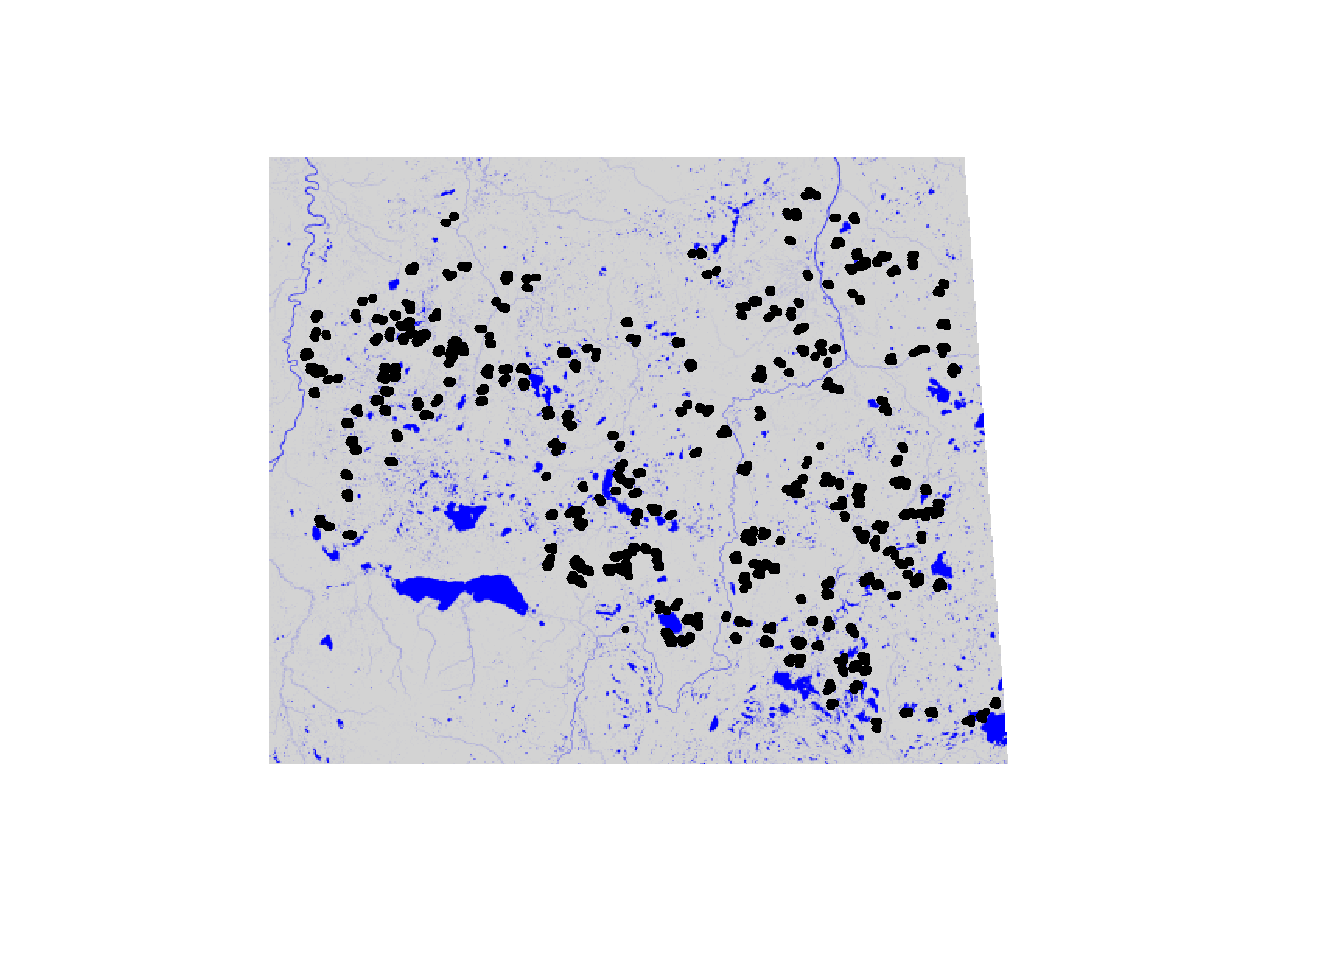
\includegraphics{qpad-book_files/figure-latex/data-xy-1.pdf}

\begin{Shaded}
\begin{Highlighting}[]
\NormalTok{cn <-}\StringTok{ }\KeywordTok{c}\NormalTok{(}\StringTok{"Open"}\NormalTok{, }\StringTok{"Water"}\NormalTok{, }\StringTok{"Agr"}\NormalTok{, }\StringTok{"UrbInd"}\NormalTok{, }\StringTok{"SoftLin"}\NormalTok{, }\StringTok{"Roads"}\NormalTok{, }
  \StringTok{"Decid"}\NormalTok{, }\StringTok{"OpenWet"}\NormalTok{, }\StringTok{"Conif"}\NormalTok{, }\StringTok{"ConifWet"}\NormalTok{)}
\CommentTok{#plot(x[,cn])}
\end{Highlighting}
\end{Shaded}

\BeginKnitrBlock{rmdexercise}
\textbf{Exercise}

Play with the data to understand the distributions and associations.
Use \texttt{summary}, \texttt{table}, \texttt{hist}, \texttt{plot}, etc.
\EndKnitrBlock{rmdexercise}

\hypertarget{regression}{%
\chapter{A Primer in Regression Techniques}\label{regression}}

\begin{quote}
All models are wrong, but some are useful -- Box
\end{quote}

\hypertarget{introduction}{%
\section{Introduction}\label{introduction}}

This chapter will provide all the foundations we need for the coming chapters.
It is not intended as a general and all-exhaustive introduction to
regression techniques, but rather the minimum requirement moving forwards.
We will also hone our data processing and plotting skills.

\hypertarget{prerequisites}{%
\section{Prerequisites}\label{prerequisites}}

\begin{Shaded}
\begin{Highlighting}[]
\KeywordTok{library}\NormalTok{(mefa4)    }\CommentTok{# Data manipulation}
\KeywordTok{library}\NormalTok{(mgcv)     }\CommentTok{# GAMs}
\KeywordTok{library}\NormalTok{(pscl)     }\CommentTok{# zero-inflated models}
\KeywordTok{library}\NormalTok{(lme4)     }\CommentTok{# GLMMs}
\KeywordTok{library}\NormalTok{(MASS)     }\CommentTok{# Negative Binomial GLM}
\KeywordTok{library}\NormalTok{(partykit) }\CommentTok{# regression trees}
\KeywordTok{library}\NormalTok{(intrval)  }\CommentTok{# interval magic}
\KeywordTok{library}\NormalTok{(opticut)  }\CommentTok{# optimal partitioning}
\KeywordTok{library}\NormalTok{(visreg)   }\CommentTok{# regression visualization}
\KeywordTok{library}\NormalTok{(MuMIn)    }\CommentTok{# multi-model inference}
\KeywordTok{source}\NormalTok{(}\StringTok{"functions.R"}\NormalTok{)}
\end{Highlighting}
\end{Shaded}

\hypertarget{poisson-null-model}{%
\section{Poisson null model}\label{poisson-null-model}}

\begin{Shaded}
\begin{Highlighting}[]
\KeywordTok{load}\NormalTok{(}\StringTok{"./_data/josm/josm.rda"}\NormalTok{)}

\NormalTok{spp <-}\StringTok{ "OVEN"} \CommentTok{# which species}

\NormalTok{ytot <-}\StringTok{ }\KeywordTok{Xtab}\NormalTok{(}\OperatorTok{~}\StringTok{ }\NormalTok{SiteID }\OperatorTok{+}\StringTok{ }\NormalTok{SpeciesID , josm}\OperatorTok{$}\NormalTok{counts[josm}\OperatorTok{$}\NormalTok{counts}\OperatorTok{$}\NormalTok{DetectType1 }\OperatorTok{!=}\StringTok{ "V"}\NormalTok{,])}
\NormalTok{ytot <-}\StringTok{ }\NormalTok{ytot[,}\KeywordTok{colSums}\NormalTok{(ytot }\OperatorTok{>}\StringTok{ }\DecValTok{0}\NormalTok{) }\OperatorTok{>}\StringTok{ }\DecValTok{0}\NormalTok{]}
\NormalTok{x <-}\StringTok{ }\KeywordTok{data.frame}\NormalTok{(}
\NormalTok{  josm}\OperatorTok{$}\NormalTok{surveys, }
  \DataTypeTok{y=}\KeywordTok{as.numeric}\NormalTok{(ytot[}\KeywordTok{rownames}\NormalTok{(x), spp]))}

\KeywordTok{table}\NormalTok{(x}\OperatorTok{$}\NormalTok{y)}
\end{Highlighting}
\end{Shaded}

\begin{verbatim}
## 
##    0    1    2    3    4    5    6 
## 2493  883  656  363  132   29   13
\end{verbatim}

\(E[Y_i] = \lambda_i = \lambda\), \((Y_i \mid \lambda) \sim Poisson(\lambda)\),
\(log(\lambda) = \beta_0\), \(\lambda = e^{\beta_0}\)

Null model

\begin{Shaded}
\begin{Highlighting}[]
\NormalTok{mP0 <-}\StringTok{ }\KeywordTok{glm}\NormalTok{(y }\OperatorTok{~}\StringTok{ }\DecValTok{1}\NormalTok{, }\DataTypeTok{data=}\NormalTok{x, }\DataTypeTok{family=}\NormalTok{poisson)}
\KeywordTok{mean}\NormalTok{(x}\OperatorTok{$}\NormalTok{y)}
\end{Highlighting}
\end{Shaded}

\begin{verbatim}
## [1] 0.8831
\end{verbatim}

\begin{Shaded}
\begin{Highlighting}[]
\KeywordTok{mean}\NormalTok{(}\KeywordTok{fitted}\NormalTok{(mP0))}
\end{Highlighting}
\end{Shaded}

\begin{verbatim}
## [1] 0.8831
\end{verbatim}

\begin{Shaded}
\begin{Highlighting}[]
\KeywordTok{exp}\NormalTok{(}\KeywordTok{coef}\NormalTok{(mP0))}
\end{Highlighting}
\end{Shaded}

\begin{verbatim}
## (Intercept) 
##      0.8831
\end{verbatim}

\begin{Shaded}
\begin{Highlighting}[]
\KeywordTok{summary}\NormalTok{(mP0)}
\end{Highlighting}
\end{Shaded}

\begin{verbatim}
## 
## Call:
## glm(formula = y ~ 1, family = poisson, data = x)
## 
## Deviance Residuals: 
##    Min      1Q  Median      3Q     Max  
##  -1.33   -1.33   -1.33    1.02    3.57  
## 
## Coefficients:
##             Estimate Std. Error z value           Pr(>|z|)    
## (Intercept)  -0.1243     0.0157   -7.89 0.0000000000000029 ***
## ---
## Signif. codes:  0 '***' 0.001 '**' 0.01 '*' 0.05 '.' 0.1 ' ' 1
## 
## (Dispersion parameter for poisson family taken to be 1)
## 
##     Null deviance: 7424.8  on 4568  degrees of freedom
## Residual deviance: 7424.8  on 4568  degrees of freedom
## AIC: 12573
## 
## Number of Fisher Scoring iterations: 6
\end{verbatim}

\hypertarget{exploring-covariates}{%
\section{Exploring covariates}\label{exploring-covariates}}

What is a useful covariate?

\begin{Shaded}
\begin{Highlighting}[]
\NormalTok{mCT <-}\StringTok{ }\KeywordTok{ctree}\NormalTok{(y }\OperatorTok{~}\StringTok{ }\NormalTok{Open }\OperatorTok{+}\StringTok{ }\NormalTok{Water }\OperatorTok{+}\StringTok{ }\NormalTok{Agr }\OperatorTok{+}\StringTok{ }\NormalTok{UrbInd }\OperatorTok{+}\StringTok{ }\NormalTok{SoftLin }\OperatorTok{+}\StringTok{ }\NormalTok{Roads }\OperatorTok{+}\StringTok{ }
\StringTok{  }\NormalTok{Decid }\OperatorTok{+}\StringTok{ }\NormalTok{OpenWet }\OperatorTok{+}\StringTok{ }\NormalTok{Conif }\OperatorTok{+}\StringTok{ }\NormalTok{ConifWet, }\DataTypeTok{data=}\NormalTok{x)}
\KeywordTok{plot}\NormalTok{(mCT, }\DataTypeTok{cex=}\FloatTok{0.5}\NormalTok{)}
\end{Highlighting}
\end{Shaded}

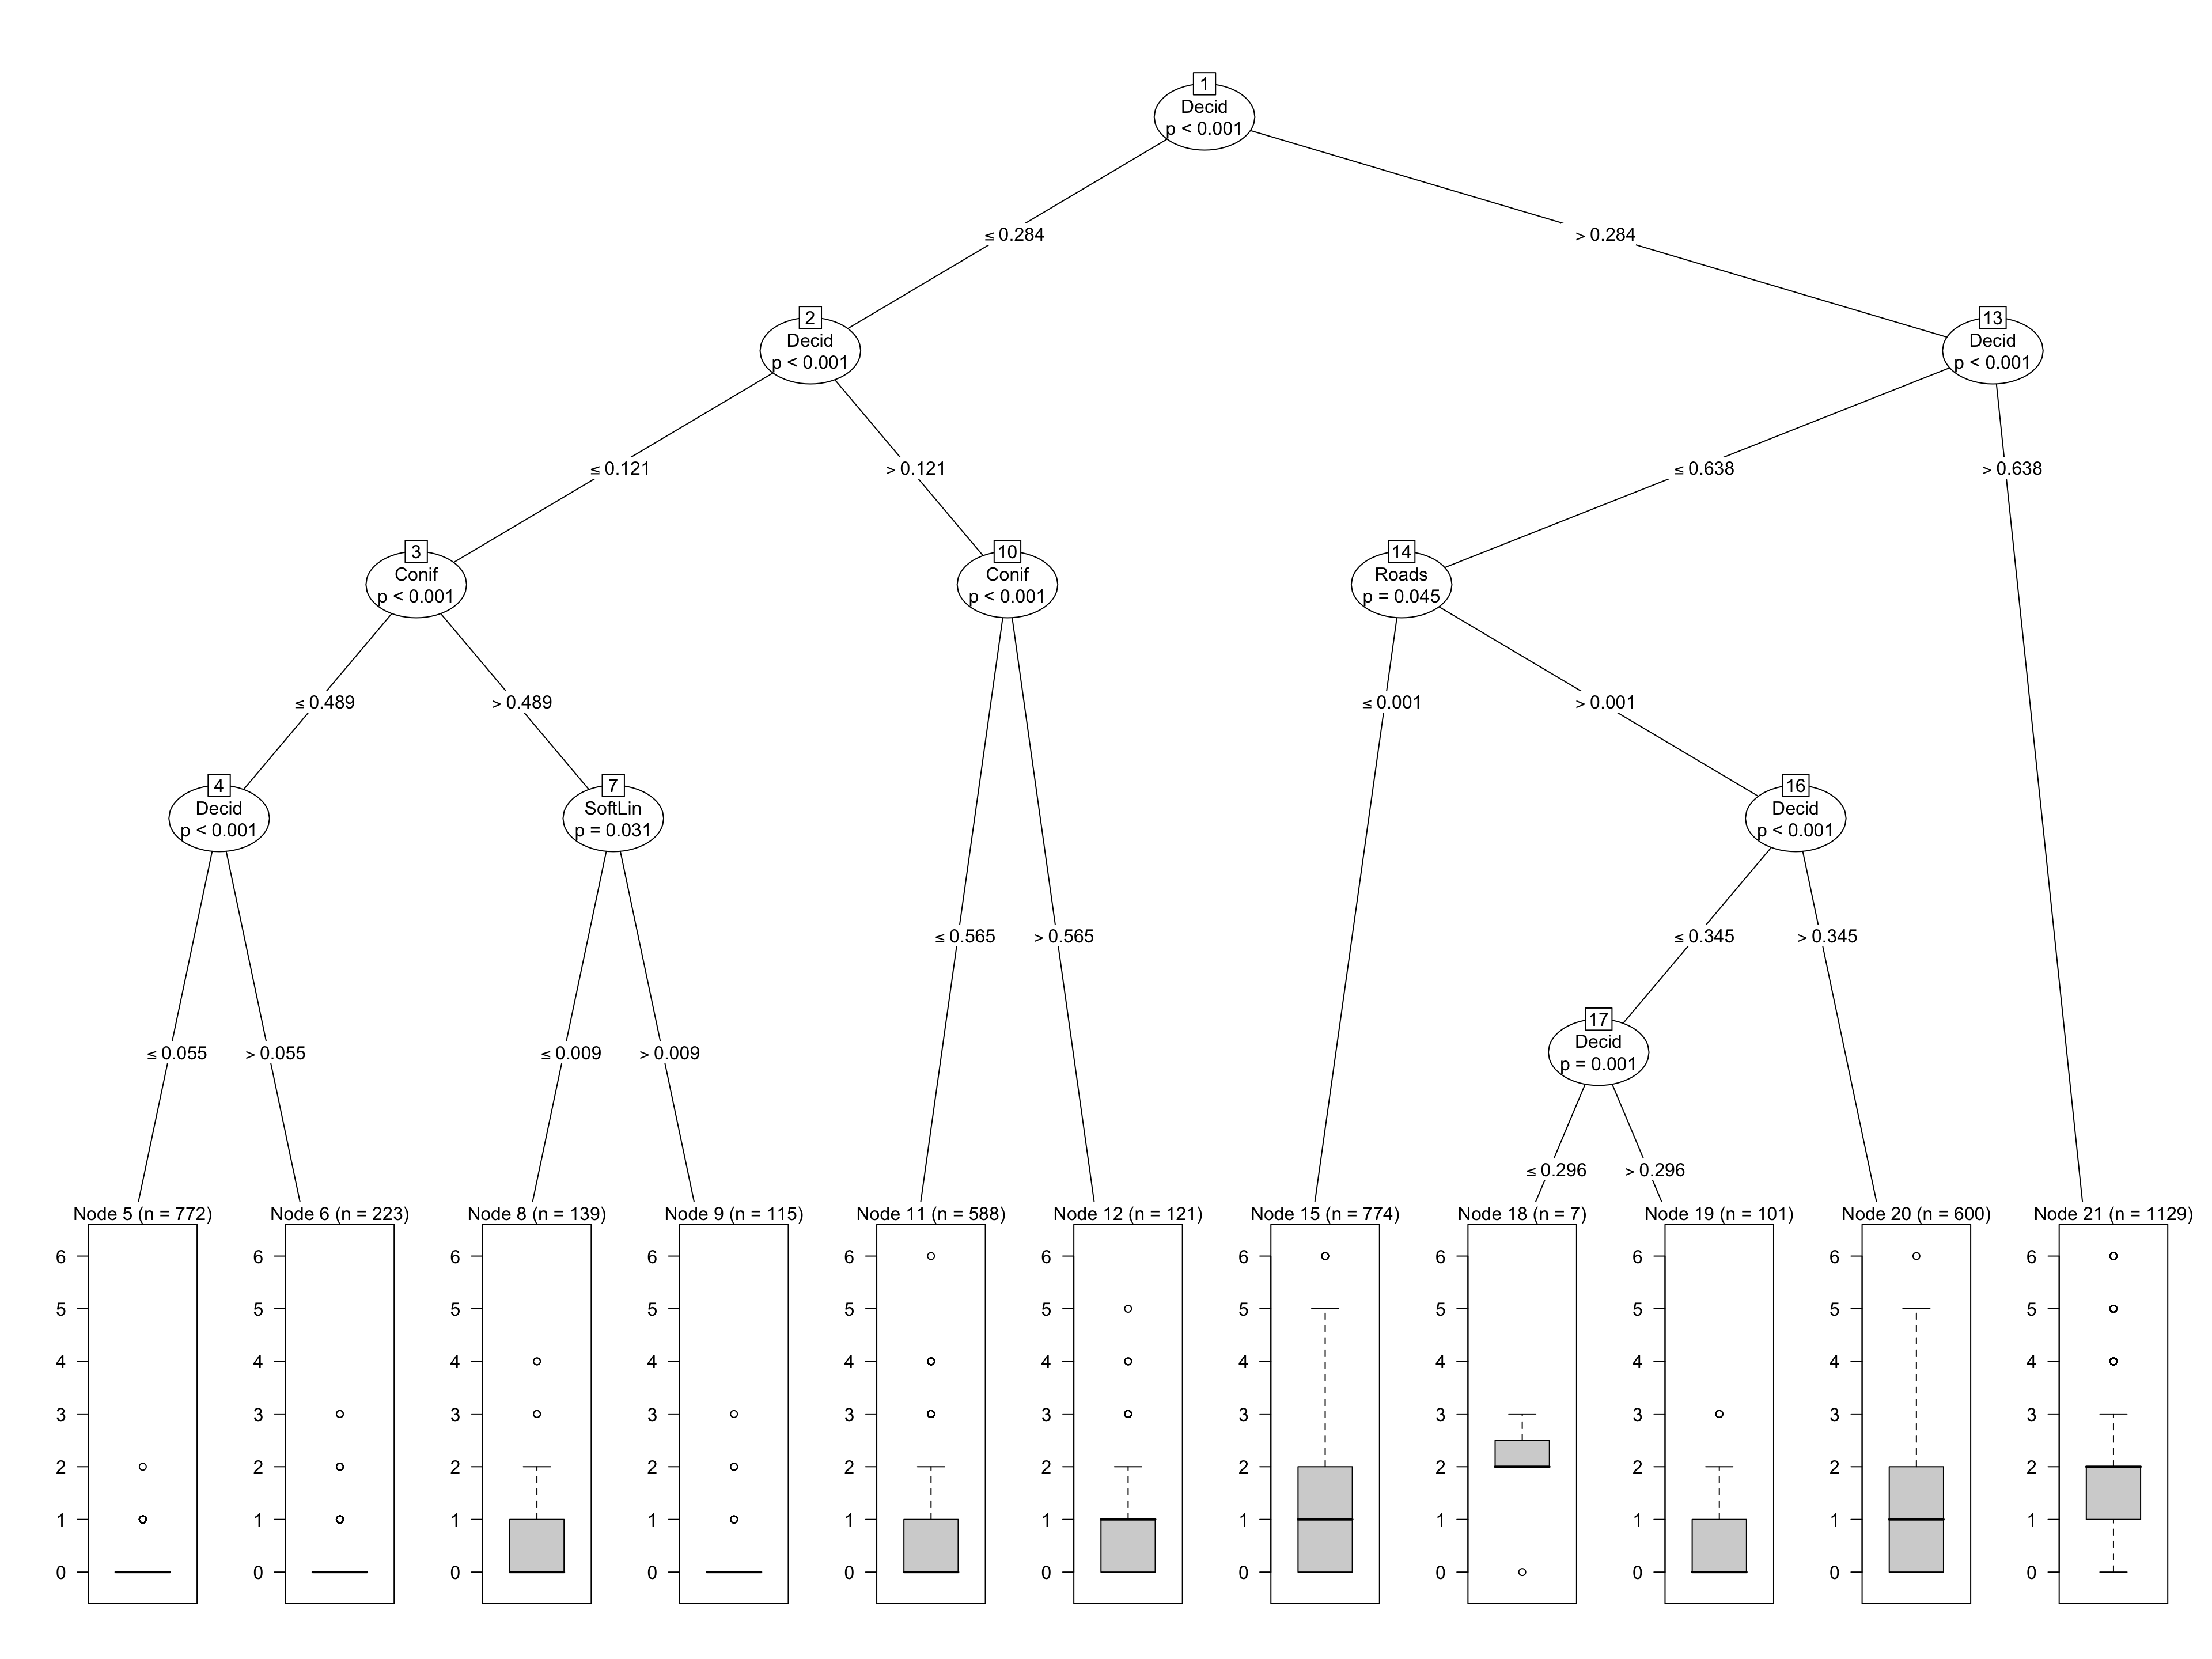
\includegraphics{qpad-book_files/figure-latex/regr-ctree-1.pdf}

\hypertarget{poisson-glm-with-one-covariate}{%
\section{Poisson GLM with one covariate}\label{poisson-glm-with-one-covariate}}

\begin{Shaded}
\begin{Highlighting}[]
\NormalTok{mP1 <-}\StringTok{ }\KeywordTok{glm}\NormalTok{(y }\OperatorTok{~}\StringTok{ }\NormalTok{Decid, }\DataTypeTok{data=}\NormalTok{x, }\DataTypeTok{family=}\NormalTok{poisson)}
\KeywordTok{mean}\NormalTok{(x}\OperatorTok{$}\NormalTok{y)}
\end{Highlighting}
\end{Shaded}

\begin{verbatim}
## [1] 0.8831
\end{verbatim}

\begin{Shaded}
\begin{Highlighting}[]
\KeywordTok{mean}\NormalTok{(}\KeywordTok{fitted}\NormalTok{(mP0))}
\end{Highlighting}
\end{Shaded}

\begin{verbatim}
## [1] 0.8831
\end{verbatim}

\begin{Shaded}
\begin{Highlighting}[]
\KeywordTok{summary}\NormalTok{(mP1)}
\end{Highlighting}
\end{Shaded}

\begin{verbatim}
## 
## Call:
## glm(formula = y ~ Decid, family = poisson, data = x)
## 
## Deviance Residuals: 
##    Min      1Q  Median      3Q     Max  
## -2.291  -0.977  -0.790   0.469   4.197  
## 
## Coefficients:
##             Estimate Std. Error z value            Pr(>|z|)    
## (Intercept)  -1.1643     0.0352   -33.1 <0.0000000000000002 ***
## Decid         2.1338     0.0537    39.7 <0.0000000000000002 ***
## ---
## Signif. codes:  0 '***' 0.001 '**' 0.01 '*' 0.05 '.' 0.1 ' ' 1
## 
## (Dispersion parameter for poisson family taken to be 1)
## 
##     Null deviance: 7424.8  on 4568  degrees of freedom
## Residual deviance: 5736.9  on 4567  degrees of freedom
## AIC: 10887
## 
## Number of Fisher Scoring iterations: 6
\end{verbatim}

\begin{Shaded}
\begin{Highlighting}[]
\KeywordTok{AIC}\NormalTok{(mP0, mP1)}

\KeywordTok{round}\NormalTok{(}\KeywordTok{rbind}\NormalTok{(}\DataTypeTok{mP0=}\KeywordTok{R2dev}\NormalTok{(mP0), }\DataTypeTok{mP1=}\KeywordTok{R2dev}\NormalTok{(mP1)), }\DecValTok{4}\NormalTok{)}
\end{Highlighting}
\end{Shaded}

\begin{verbatim}
##         R2  R2adj Deviance Dev0 DevR  df0  dfR p_value
## mP0 0.0000 0.0000        0 7425 7425 4568 4568       0
## mP1 0.2273 0.2272     1688 7425 5737 4568 4567       0
\end{verbatim}

\begin{Shaded}
\begin{Highlighting}[]
\NormalTok{xnew <-}\StringTok{ }\KeywordTok{data.frame}\NormalTok{(}\DataTypeTok{Decid=}\KeywordTok{seq}\NormalTok{(}\DecValTok{0}\NormalTok{, }\DecValTok{1}\NormalTok{, }\FloatTok{0.01}\NormalTok{))}
\NormalTok{CI0 <-}\StringTok{ }\KeywordTok{predict_sim}\NormalTok{(mP0, xnew, }\DataTypeTok{interval=}\StringTok{"confidence"}\NormalTok{, }\DataTypeTok{level=}\FloatTok{0.95}\NormalTok{, }\DataTypeTok{B=}\DecValTok{999}\NormalTok{)}
\NormalTok{PI0 <-}\StringTok{ }\KeywordTok{predict_sim}\NormalTok{(mP0, xnew, }\DataTypeTok{interval=}\StringTok{"prediction"}\NormalTok{, }\DataTypeTok{level=}\FloatTok{0.95}\NormalTok{, }\DataTypeTok{B=}\DecValTok{999}\NormalTok{)}
\NormalTok{CI1 <-}\StringTok{ }\KeywordTok{predict_sim}\NormalTok{(mP1, xnew, }\DataTypeTok{interval=}\StringTok{"confidence"}\NormalTok{, }\DataTypeTok{level=}\FloatTok{0.95}\NormalTok{, }\DataTypeTok{B=}\DecValTok{999}\NormalTok{)}
\NormalTok{PI1 <-}\StringTok{ }\KeywordTok{predict_sim}\NormalTok{(mP1, xnew, }\DataTypeTok{interval=}\StringTok{"prediction"}\NormalTok{, }\DataTypeTok{level=}\FloatTok{0.95}\NormalTok{, }\DataTypeTok{B=}\DecValTok{999}\NormalTok{)}

\CommentTok{## nominal coverage is 95%}
\KeywordTok{sum}\NormalTok{(x}\OperatorTok{$}\NormalTok{y }\OperatorTok\StringTok{ }\KeywordTok{predict_sim}\NormalTok{(mP0, }\DataTypeTok{interval=}\StringTok{"prediction"}\NormalTok{, }\DataTypeTok{level=}\FloatTok{0.95}\NormalTok{, }\DataTypeTok{B=}\DecValTok{999}\NormalTok{)[,}\KeywordTok{c}\NormalTok{(}\StringTok{"lwr"}\NormalTok{, }\StringTok{"upr"}\NormalTok{)]) }\OperatorTok{/}\StringTok{ }\KeywordTok{nrow}\NormalTok{(x)}
\end{Highlighting}
\end{Shaded}

\begin{verbatim}
## [1] 0.9619
\end{verbatim}

\begin{Shaded}
\begin{Highlighting}[]
\KeywordTok{sum}\NormalTok{(x}\OperatorTok{$}\NormalTok{y }\OperatorTok\StringTok{ }\KeywordTok{predict_sim}\NormalTok{(mP1, }\DataTypeTok{interval=}\StringTok{"prediction"}\NormalTok{, }\DataTypeTok{level=}\FloatTok{0.95}\NormalTok{, }\DataTypeTok{B=}\DecValTok{999}\NormalTok{)[,}\KeywordTok{c}\NormalTok{(}\StringTok{"lwr"}\NormalTok{, }\StringTok{"upr"}\NormalTok{)]) }\OperatorTok{/}\StringTok{ }\KeywordTok{nrow}\NormalTok{(x)}
\end{Highlighting}
\end{Shaded}

\begin{verbatim}
## [1] 0.9709
\end{verbatim}

\hypertarget{additive-model}{%
\section{Additive model}\label{additive-model}}

\begin{Shaded}
\begin{Highlighting}[]
\NormalTok{mGAM <-}\StringTok{ }\NormalTok{mgcv}\OperatorTok{::}\KeywordTok{gam}\NormalTok{(y }\OperatorTok{~}\StringTok{ }\KeywordTok{s}\NormalTok{(Decid), x, }\DataTypeTok{family=}\NormalTok{poisson)}
\KeywordTok{plot}\NormalTok{(mGAM)}
\end{Highlighting}
\end{Shaded}

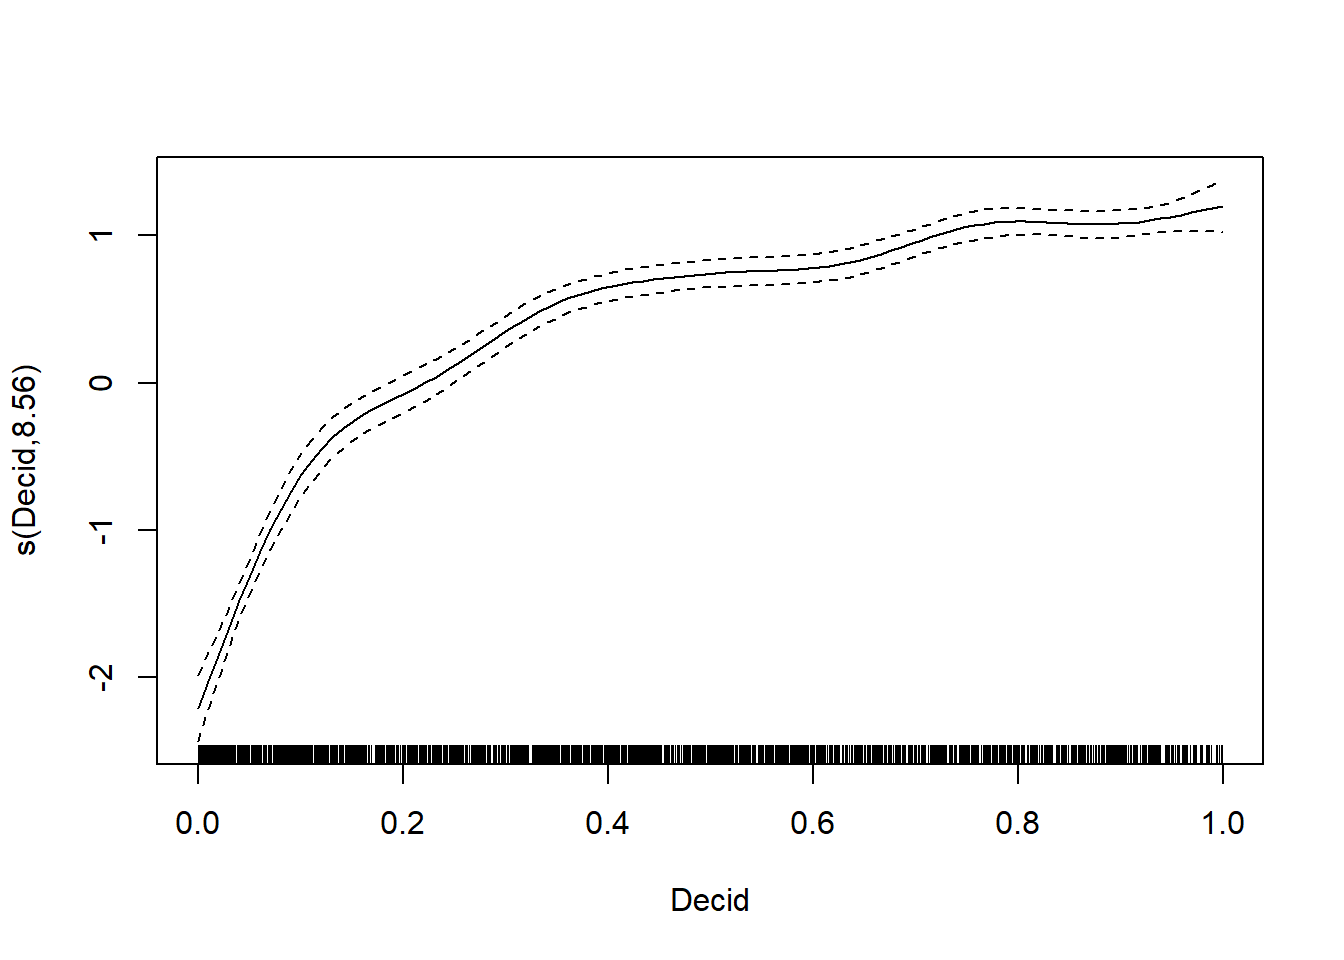
\includegraphics{qpad-book_files/figure-latex/unnamed-chunk-27-1.pdf}

\begin{Shaded}
\begin{Highlighting}[]
\NormalTok{fitCT <-}\StringTok{ }\KeywordTok{predict}\NormalTok{(mCT, x[}\KeywordTok{order}\NormalTok{(x}\OperatorTok{$}\NormalTok{Decid),])}
\NormalTok{fitGAM <-}\StringTok{ }\KeywordTok{predict}\NormalTok{(mGAM, xnew, }\DataTypeTok{type=}\StringTok{"response"}\NormalTok{)}

\NormalTok{op <-}\StringTok{ }\KeywordTok{par}\NormalTok{(}\DataTypeTok{mfrow=}\KeywordTok{c}\NormalTok{(}\DecValTok{2}\NormalTok{,}\DecValTok{2}\NormalTok{))}
\KeywordTok{plot}\NormalTok{(}\KeywordTok{jitter}\NormalTok{(y, }\FloatTok{0.5}\NormalTok{) }\OperatorTok{~}\StringTok{ }\NormalTok{Decid, x, }\DataTypeTok{xlab=}\StringTok{"Decid"}\NormalTok{, }\DataTypeTok{ylab=}\StringTok{"E[Y]"}\NormalTok{,}
  \DataTypeTok{ylim=}\KeywordTok{c}\NormalTok{(}\DecValTok{0}\NormalTok{, }\KeywordTok{max}\NormalTok{(PI1}\OperatorTok{$}\NormalTok{upr)}\OperatorTok{+}\DecValTok{1}\NormalTok{), }\DataTypeTok{pch=}\DecValTok{19}\NormalTok{, }\DataTypeTok{col=}\StringTok{"#bbbbbb33"}\NormalTok{, }\DataTypeTok{main=}\StringTok{"P0"}\NormalTok{)}
\KeywordTok{lines}\NormalTok{(CI0}\OperatorTok{$}\NormalTok{fit }\OperatorTok{~}\StringTok{ }\NormalTok{xnew}\OperatorTok{$}\NormalTok{Decid, }\DataTypeTok{lty=}\DecValTok{1}\NormalTok{, }\DataTypeTok{col=}\DecValTok{4}\NormalTok{)}
\KeywordTok{lines}\NormalTok{(CI0}\OperatorTok{$}\NormalTok{lwr }\OperatorTok{~}\StringTok{ }\NormalTok{xnew}\OperatorTok{$}\NormalTok{Decid, }\DataTypeTok{lty=}\DecValTok{2}\NormalTok{, }\DataTypeTok{col=}\DecValTok{4}\NormalTok{)}
\KeywordTok{lines}\NormalTok{(CI0}\OperatorTok{$}\NormalTok{upr }\OperatorTok{~}\StringTok{ }\NormalTok{xnew}\OperatorTok{$}\NormalTok{Decid, }\DataTypeTok{lty=}\DecValTok{2}\NormalTok{, }\DataTypeTok{col=}\DecValTok{4}\NormalTok{)}
\KeywordTok{lines}\NormalTok{(PI0}\OperatorTok{$}\NormalTok{lwr }\OperatorTok{~}\StringTok{ }\NormalTok{xnew}\OperatorTok{$}\NormalTok{Decid, }\DataTypeTok{lty=}\DecValTok{3}\NormalTok{, }\DataTypeTok{col=}\DecValTok{4}\NormalTok{)}
\KeywordTok{lines}\NormalTok{(PI0}\OperatorTok{$}\NormalTok{upr }\OperatorTok{~}\StringTok{ }\NormalTok{xnew}\OperatorTok{$}\NormalTok{Decid, }\DataTypeTok{lty=}\DecValTok{3}\NormalTok{, }\DataTypeTok{col=}\DecValTok{4}\NormalTok{)}

\KeywordTok{plot}\NormalTok{(}\KeywordTok{jitter}\NormalTok{(y, }\FloatTok{0.5}\NormalTok{) }\OperatorTok{~}\StringTok{ }\NormalTok{Decid, x, }\DataTypeTok{xlab=}\StringTok{"Decid"}\NormalTok{, }\DataTypeTok{ylab=}\StringTok{"E[Y]"}\NormalTok{,}
  \DataTypeTok{ylim=}\KeywordTok{c}\NormalTok{(}\DecValTok{0}\NormalTok{, }\KeywordTok{max}\NormalTok{(PI1}\OperatorTok{$}\NormalTok{upr)}\OperatorTok{+}\DecValTok{1}\NormalTok{), }\DataTypeTok{pch=}\DecValTok{19}\NormalTok{, }\DataTypeTok{col=}\StringTok{"#bbbbbb33"}\NormalTok{, }\DataTypeTok{main=}\StringTok{"P1"}\NormalTok{)}
\KeywordTok{lines}\NormalTok{(CI1}\OperatorTok{$}\NormalTok{fit }\OperatorTok{~}\StringTok{ }\NormalTok{xnew}\OperatorTok{$}\NormalTok{Decid, }\DataTypeTok{lty=}\DecValTok{1}\NormalTok{, }\DataTypeTok{col=}\DecValTok{4}\NormalTok{)}
\KeywordTok{lines}\NormalTok{(CI1}\OperatorTok{$}\NormalTok{lwr }\OperatorTok{~}\StringTok{ }\NormalTok{xnew}\OperatorTok{$}\NormalTok{Decid, }\DataTypeTok{lty=}\DecValTok{2}\NormalTok{, }\DataTypeTok{col=}\DecValTok{4}\NormalTok{)}
\KeywordTok{lines}\NormalTok{(CI1}\OperatorTok{$}\NormalTok{upr }\OperatorTok{~}\StringTok{ }\NormalTok{xnew}\OperatorTok{$}\NormalTok{Decid, }\DataTypeTok{lty=}\DecValTok{2}\NormalTok{, }\DataTypeTok{col=}\DecValTok{4}\NormalTok{)}
\KeywordTok{lines}\NormalTok{(PI1}\OperatorTok{$}\NormalTok{lwr }\OperatorTok{~}\StringTok{ }\NormalTok{xnew}\OperatorTok{$}\NormalTok{Decid, }\DataTypeTok{lty=}\DecValTok{3}\NormalTok{, }\DataTypeTok{col=}\DecValTok{4}\NormalTok{)}
\KeywordTok{lines}\NormalTok{(PI1}\OperatorTok{$}\NormalTok{upr }\OperatorTok{~}\StringTok{ }\NormalTok{xnew}\OperatorTok{$}\NormalTok{Decid, }\DataTypeTok{lty=}\DecValTok{3}\NormalTok{, }\DataTypeTok{col=}\DecValTok{4}\NormalTok{)}

\KeywordTok{plot}\NormalTok{(}\KeywordTok{jitter}\NormalTok{(y, }\FloatTok{0.5}\NormalTok{) }\OperatorTok{~}\StringTok{ }\NormalTok{Decid, x, }\DataTypeTok{xlab=}\StringTok{"Decid"}\NormalTok{, }\DataTypeTok{ylab=}\StringTok{"E[Y]"}\NormalTok{,}
  \DataTypeTok{ylim=}\KeywordTok{c}\NormalTok{(}\DecValTok{0}\NormalTok{, }\KeywordTok{max}\NormalTok{(PI1}\OperatorTok{$}\NormalTok{upr)}\OperatorTok{+}\DecValTok{1}\NormalTok{), }\DataTypeTok{pch=}\DecValTok{19}\NormalTok{, }\DataTypeTok{col=}\StringTok{"#bbbbbb33"}\NormalTok{, }\DataTypeTok{main=}\StringTok{"ctree"}\NormalTok{)}
\KeywordTok{lines}\NormalTok{(fitCT }\OperatorTok{~}\StringTok{ }\NormalTok{x}\OperatorTok{$}\NormalTok{Decid[}\KeywordTok{order}\NormalTok{(x}\OperatorTok{$}\NormalTok{Decid)], }\DataTypeTok{lty=}\DecValTok{1}\NormalTok{, }\DataTypeTok{col=}\DecValTok{4}\NormalTok{)}

\KeywordTok{plot}\NormalTok{(}\KeywordTok{jitter}\NormalTok{(y, }\FloatTok{0.5}\NormalTok{) }\OperatorTok{~}\StringTok{ }\NormalTok{Decid, x, }\DataTypeTok{xlab=}\StringTok{"Decid"}\NormalTok{, }\DataTypeTok{ylab=}\StringTok{"E[Y]"}\NormalTok{,}
  \DataTypeTok{ylim=}\KeywordTok{c}\NormalTok{(}\DecValTok{0}\NormalTok{, }\KeywordTok{max}\NormalTok{(PI1}\OperatorTok{$}\NormalTok{upr)}\OperatorTok{+}\DecValTok{1}\NormalTok{), }\DataTypeTok{pch=}\DecValTok{19}\NormalTok{, }\DataTypeTok{col=}\StringTok{"#bbbbbb33"}\NormalTok{, }\DataTypeTok{main=}\StringTok{"GAM"}\NormalTok{)}
\KeywordTok{lines}\NormalTok{(fitGAM }\OperatorTok{~}\StringTok{ }\NormalTok{xnew}\OperatorTok{$}\NormalTok{Decid, }\DataTypeTok{lty=}\DecValTok{1}\NormalTok{, }\DataTypeTok{col=}\DecValTok{4}\NormalTok{)}
\end{Highlighting}
\end{Shaded}

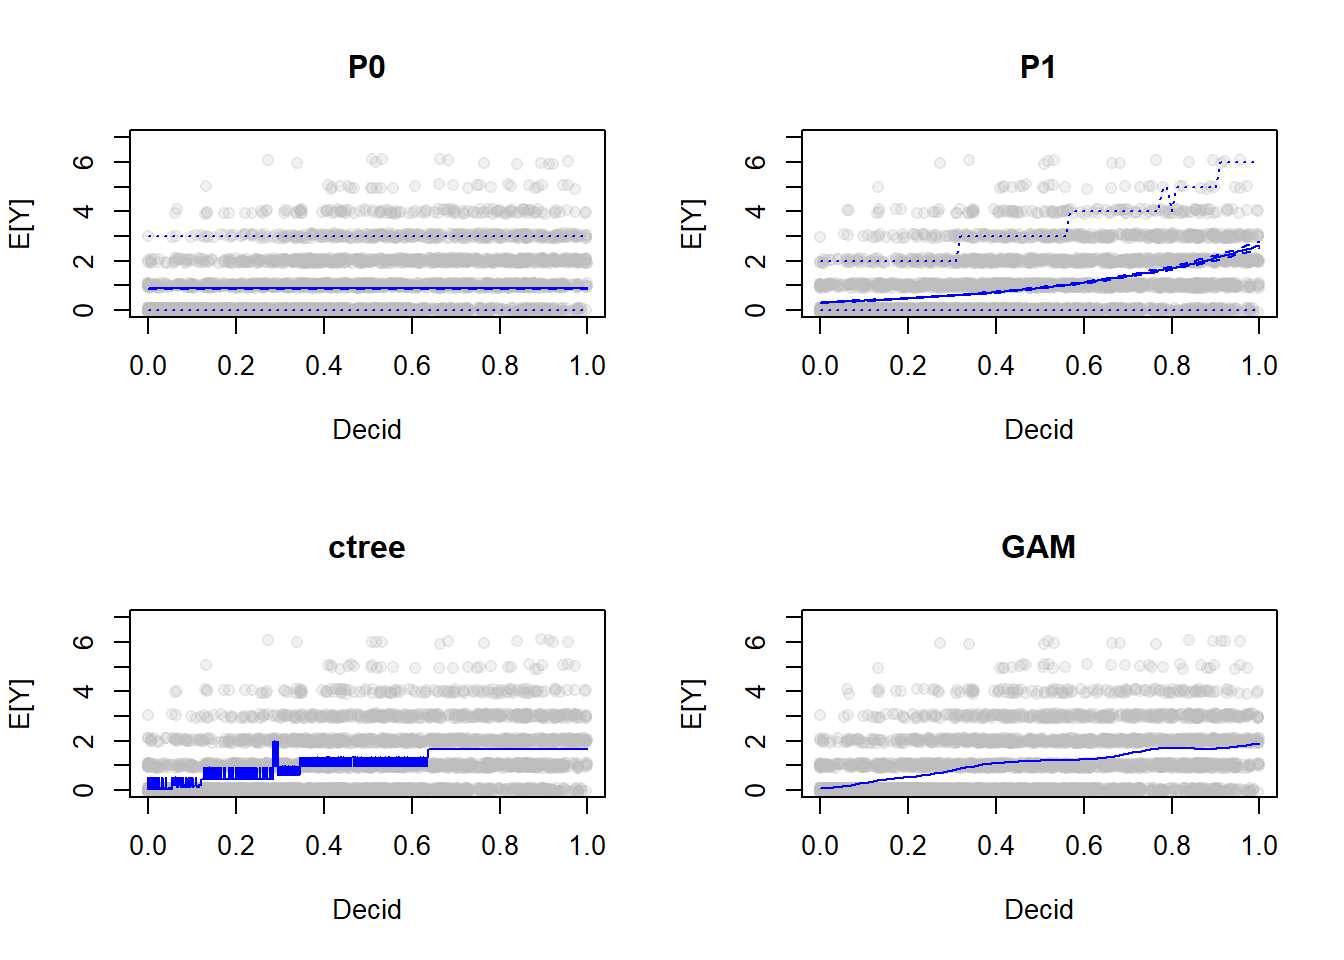
\includegraphics{qpad-book_files/figure-latex/unnamed-chunk-27-2.pdf}

\begin{Shaded}
\begin{Highlighting}[]
\KeywordTok{par}\NormalTok{(op)}
\end{Highlighting}
\end{Shaded}

\BeginKnitrBlock{rmdexercise}
\textbf{Exercise}

Play with GAM and other variables to understand responses:
\texttt{plot(mgcv::gam(y\ \textasciitilde{}\ s(\textless{}variable\_name\textgreater{}),\ data=x,\ family=poisson))}
\EndKnitrBlock{rmdexercise}

\hypertarget{multiple-main-effects}{%
\section{Multiple main effects}\label{multiple-main-effects}}

\begin{Shaded}
\begin{Highlighting}[]
\NormalTok{mP2 <-}\StringTok{ }\KeywordTok{step}\NormalTok{(}\KeywordTok{glm}\NormalTok{(y }\OperatorTok{~}\StringTok{ }\NormalTok{Open }\OperatorTok{+}\StringTok{ }\NormalTok{Agr }\OperatorTok{+}\StringTok{ }\NormalTok{UrbInd }\OperatorTok{+}\StringTok{ }\NormalTok{SoftLin }\OperatorTok{+}\StringTok{ }\NormalTok{Roads }\OperatorTok{+}\StringTok{ }
\StringTok{  }\NormalTok{Decid }\OperatorTok{+}\StringTok{ }\NormalTok{OpenWet }\OperatorTok{+}\StringTok{ }\NormalTok{Conif }\OperatorTok{+}\StringTok{ }\NormalTok{ConifWet }\OperatorTok{+}\StringTok{ }
\StringTok{  }\NormalTok{OvernightRain }\OperatorTok{+}\StringTok{ }\NormalTok{TSSR }\OperatorTok{+}\StringTok{ }\NormalTok{DAY }\OperatorTok{+}\StringTok{ }\NormalTok{Longitude }\OperatorTok{+}\StringTok{ }\NormalTok{Latitude,}
  \DataTypeTok{data=}\NormalTok{x, }\DataTypeTok{family=}\NormalTok{poisson), }\DataTypeTok{trace=}\DecValTok{0}\NormalTok{)}

\KeywordTok{summary}\NormalTok{(mP2)}
\end{Highlighting}
\end{Shaded}

\begin{verbatim}
## 
## Call:
## glm(formula = y ~ Open + UrbInd + Decid + OpenWet + Conif + ConifWet + 
##     TSSR + DAY + Longitude + Latitude, family = poisson, data = x)
## 
## Deviance Residuals: 
##    Min      1Q  Median      3Q     Max  
## -2.763  -0.986  -0.674   0.451   4.624  
## 
## Coefficients:
##             Estimate Std. Error z value             Pr(>|z|)    
## (Intercept) -5.88293    1.30223   -4.52      0.0000062546826 ***
## Open        -3.47428    0.65867   -5.27      0.0000001330000 ***
## UrbInd      -1.66883    0.54216   -3.08              0.00208 ** 
## Decid        0.83372    0.25957    3.21              0.00132 ** 
## OpenWet     -0.74076    0.30238   -2.45              0.01430 *  
## Conif       -0.88558    0.26566   -3.33              0.00086 ***
## ConifWet    -1.89423    0.27170   -6.97      0.0000000000031 ***
## TSSR        -1.23416    0.24984   -4.94      0.0000007818641 ***
## DAY         -2.87970    0.52686   -5.47      0.0000000460898 ***
## Longitude    0.03831    0.00877    4.37      0.0000124210771 ***
## Latitude     0.20930    0.02309    9.06 < 0.0000000000000002 ***
## ---
## Signif. codes:  0 '***' 0.001 '**' 0.01 '*' 0.05 '.' 0.1 ' ' 1
## 
## (Dispersion parameter for poisson family taken to be 1)
## 
##     Null deviance: 7424.8  on 4568  degrees of freedom
## Residual deviance: 5501.1  on 4558  degrees of freedom
## AIC: 10669
## 
## Number of Fisher Scoring iterations: 6
\end{verbatim}

\begin{Shaded}
\begin{Highlighting}[]
\KeywordTok{AIC}\NormalTok{(mP0, mP1, mP2)}

\KeywordTok{round}\NormalTok{(}\KeywordTok{rbind}\NormalTok{(}\DataTypeTok{mP0=}\KeywordTok{R2dev}\NormalTok{(mP0), }\DataTypeTok{mP1=}\KeywordTok{R2dev}\NormalTok{(mP1), }\DataTypeTok{mP2=}\KeywordTok{R2dev}\NormalTok{(mP2)), }\DecValTok{4}\NormalTok{)}
\end{Highlighting}
\end{Shaded}

\begin{verbatim}
##         R2  R2adj Deviance Dev0 DevR  df0  dfR p_value
## mP0 0.0000 0.0000        0 7425 7425 4568 4568       0
## mP1 0.2273 0.2272     1688 7425 5737 4568 4567       0
## mP2 0.2591 0.2575     1924 7425 5501 4568 4558       0
\end{verbatim}

\hypertarget{nonlinear-terms}{%
\section{Nonlinear terms}\label{nonlinear-terms}}

Polynomials

\begin{Shaded}
\begin{Highlighting}[]
\NormalTok{mP12 <-}\StringTok{ }\KeywordTok{glm}\NormalTok{(y }\OperatorTok{~}\StringTok{ }\NormalTok{Decid }\OperatorTok{+}\StringTok{ }\KeywordTok{I}\NormalTok{(Decid}\OperatorTok{^}\DecValTok{2}\NormalTok{), }\DataTypeTok{data=}\NormalTok{x, }\DataTypeTok{family=}\NormalTok{poisson)}
\NormalTok{mP13 <-}\StringTok{ }\KeywordTok{glm}\NormalTok{(y }\OperatorTok{~}\StringTok{ }\NormalTok{Decid }\OperatorTok{+}\StringTok{ }\KeywordTok{I}\NormalTok{(Decid}\OperatorTok{^}\DecValTok{2}\NormalTok{) }\OperatorTok{+}\StringTok{ }\KeywordTok{I}\NormalTok{(Decid}\OperatorTok{^}\DecValTok{3}\NormalTok{), }\DataTypeTok{data=}\NormalTok{x, }\DataTypeTok{family=}\NormalTok{poisson)}
\NormalTok{mP14 <-}\StringTok{ }\KeywordTok{glm}\NormalTok{(y }\OperatorTok{~}\StringTok{ }\NormalTok{Decid }\OperatorTok{+}\StringTok{ }\KeywordTok{I}\NormalTok{(Decid}\OperatorTok{^}\DecValTok{2}\NormalTok{) }\OperatorTok{+}\StringTok{ }\KeywordTok{I}\NormalTok{(Decid}\OperatorTok{^}\DecValTok{3}\NormalTok{) }\OperatorTok{+}\StringTok{ }\KeywordTok{I}\NormalTok{(Decid}\OperatorTok{^}\DecValTok{4}\NormalTok{), }\DataTypeTok{data=}\NormalTok{x, }\DataTypeTok{family=}\NormalTok{poisson)}
\KeywordTok{AIC}\NormalTok{(mP1, mP12, mP13, mP14)}

\NormalTok{pr <-}\StringTok{ }\KeywordTok{cbind}\NormalTok{(}
  \KeywordTok{predict}\NormalTok{(mP1, xnew, }\DataTypeTok{type=}\StringTok{"response"}\NormalTok{),}
  \KeywordTok{predict}\NormalTok{(mP12, xnew, }\DataTypeTok{type=}\StringTok{"response"}\NormalTok{),}
  \KeywordTok{predict}\NormalTok{(mP13, xnew, }\DataTypeTok{type=}\StringTok{"response"}\NormalTok{),}
  \KeywordTok{predict}\NormalTok{(mP14, xnew, }\DataTypeTok{type=}\StringTok{"response"}\NormalTok{),}
\NormalTok{  fitGAM)}
\KeywordTok{matplot}\NormalTok{(xnew}\OperatorTok{$}\NormalTok{Decid, pr, }\DataTypeTok{lty=}\DecValTok{1}\NormalTok{, }\DataTypeTok{type=}\StringTok{"l"}\NormalTok{)}
\end{Highlighting}
\end{Shaded}

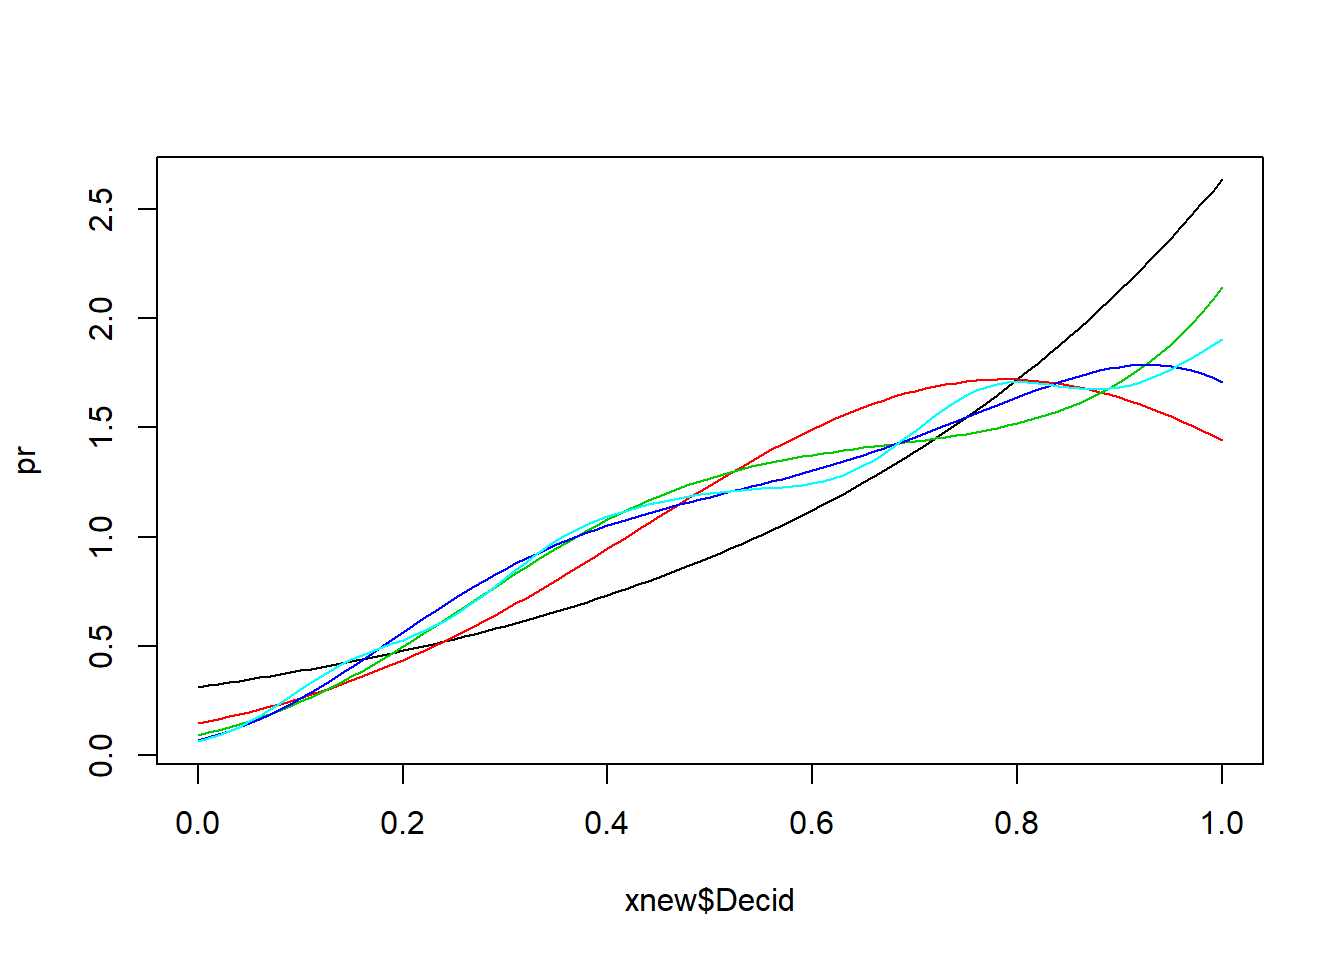
\includegraphics{qpad-book_files/figure-latex/unnamed-chunk-30-1.pdf}

\hypertarget{categorical-variables}{%
\section{Categorical variables}\label{categorical-variables}}

Categories

\begin{Shaded}
\begin{Highlighting}[]
\NormalTok{cn <-}\StringTok{ }\KeywordTok{c}\NormalTok{(}\StringTok{"Open"}\NormalTok{, }\StringTok{"Water"}\NormalTok{, }\StringTok{"Agr"}\NormalTok{, }\StringTok{"UrbInd"}\NormalTok{, }\StringTok{"SoftLin"}\NormalTok{, }\StringTok{"Roads"}\NormalTok{, }\StringTok{"Decid"}\NormalTok{, }
  \StringTok{"OpenWet"}\NormalTok{, }\StringTok{"Conif"}\NormalTok{, }\StringTok{"ConifWet"}\NormalTok{)}
\NormalTok{h <-}\StringTok{ }\KeywordTok{find_max}\NormalTok{(x[,cn])}
\KeywordTok{hist}\NormalTok{(h}\OperatorTok{$}\NormalTok{value)}
\end{Highlighting}
\end{Shaded}

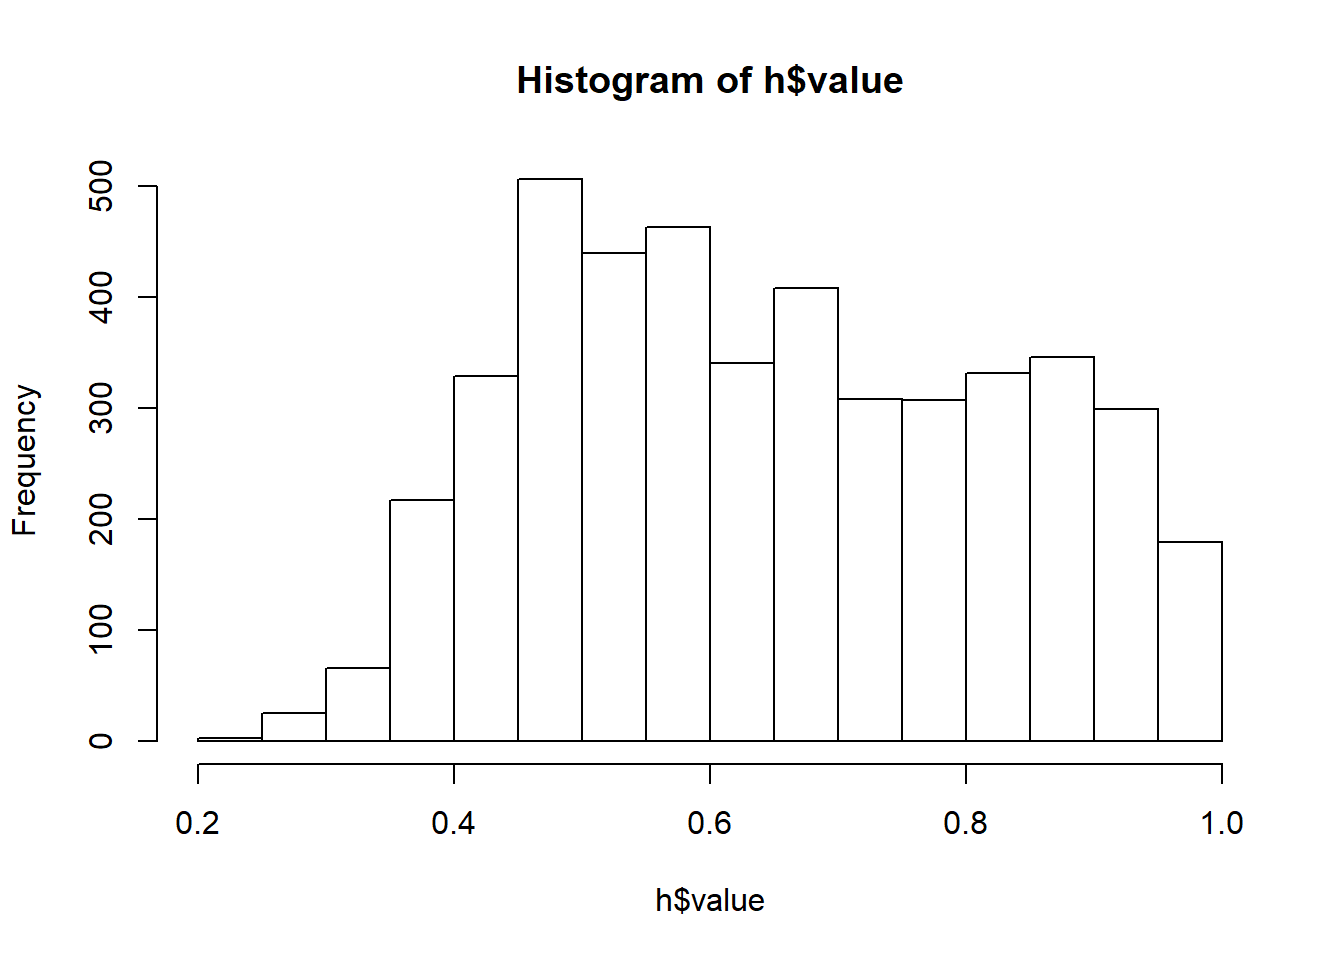
\includegraphics{qpad-book_files/figure-latex/unnamed-chunk-31-1.pdf}

\begin{Shaded}
\begin{Highlighting}[]
\KeywordTok{table}\NormalTok{(h}\OperatorTok{$}\NormalTok{index)}
\end{Highlighting}
\end{Shaded}

\begin{verbatim}
## 
##     Open    Water      Agr   UrbInd  SoftLin    Roads    Decid 
##       12       10        4       14        0        2     2084 
##  OpenWet    Conif ConifWet 
##      160      745     1538
\end{verbatim}

\begin{Shaded}
\begin{Highlighting}[]
\NormalTok{x}\OperatorTok{$}\NormalTok{hab <-}\StringTok{ }\KeywordTok{droplevels}\NormalTok{(h}\OperatorTok{$}\NormalTok{index)}

\NormalTok{mP3 <-}\StringTok{ }\KeywordTok{glm}\NormalTok{(y }\OperatorTok{~}\StringTok{ }\NormalTok{hab, }\DataTypeTok{data=}\NormalTok{x, }\DataTypeTok{family=}\NormalTok{poisson)}

\KeywordTok{summary}\NormalTok{(mP3)}
\end{Highlighting}
\end{Shaded}

\begin{verbatim}
## 
## Call:
## glm(formula = y ~ hab, family = poisson, data = x)
## 
## Deviance Residuals: 
##    Min      1Q  Median      3Q     Max  
## -1.691  -0.873  -0.817   0.449   4.832  
## 
## Coefficients:
##             Estimate Std. Error z value Pr(>|z|)   
## (Intercept)   -1.386      0.577   -2.40   0.0163 * 
## habWater       1.030      0.690    1.49   0.1357   
## habAgr         0.693      0.913    0.76   0.4477   
## habUrbInd      0.134      0.764    0.17   0.8612   
## habRoads     -10.916    201.285   -0.05   0.9567   
## habDecid       1.744      0.578    3.02   0.0025 **
## habOpenWet     0.422      0.591    0.71   0.4755   
## habConif       0.913      0.579    1.58   0.1150   
## habConifWet    0.288      0.579    0.50   0.6185   
## ---
## Signif. codes:  0 '***' 0.001 '**' 0.01 '*' 0.05 '.' 0.1 ' ' 1
## 
## (Dispersion parameter for poisson family taken to be 1)
## 
##     Null deviance: 7424.8  on 4568  degrees of freedom
## Residual deviance: 5997.2  on 4560  degrees of freedom
## AIC: 11161
## 
## Number of Fisher Scoring iterations: 10
\end{verbatim}

\begin{Shaded}
\begin{Highlighting}[]
\KeywordTok{AIC}\NormalTok{(mP0, mP1, mP2, mP3)}

\KeywordTok{round}\NormalTok{(}\KeywordTok{rbind}\NormalTok{(}\DataTypeTok{mP0=}\KeywordTok{R2dev}\NormalTok{(mP0), }\DataTypeTok{mP1=}\KeywordTok{R2dev}\NormalTok{(mP1), }\DataTypeTok{mP2=}\KeywordTok{R2dev}\NormalTok{(mP2), }\DataTypeTok{mP3=}\KeywordTok{R2dev}\NormalTok{(mP3)), }\DecValTok{4}\NormalTok{)}
\end{Highlighting}
\end{Shaded}

\begin{verbatim}
##         R2  R2adj Deviance Dev0 DevR  df0  dfR p_value
## mP0 0.0000 0.0000        0 7425 7425 4568 4568       0
## mP1 0.2273 0.2272     1688 7425 5737 4568 4567       0
## mP2 0.2591 0.2575     1924 7425 5501 4568 4558       0
## mP3 0.1923 0.1909     1428 7425 5997 4568 4560       0
\end{verbatim}

\hypertarget{optimal-partitioning}{%
\subsection{Optimal partitioning}\label{optimal-partitioning}}

\begin{Shaded}
\begin{Highlighting}[]
\NormalTok{oc <-}\StringTok{ }\KeywordTok{opticut}\NormalTok{(}\KeywordTok{as.matrix}\NormalTok{(ytot) }\OperatorTok{~}\StringTok{ }\DecValTok{1}\NormalTok{, }\DataTypeTok{strata =}\NormalTok{ x}\OperatorTok{$}\NormalTok{hab, }\DataTypeTok{dist=}\StringTok{"poisson"}\NormalTok{)}
\KeywordTok{plot}\NormalTok{(oc)}
\end{Highlighting}
\end{Shaded}

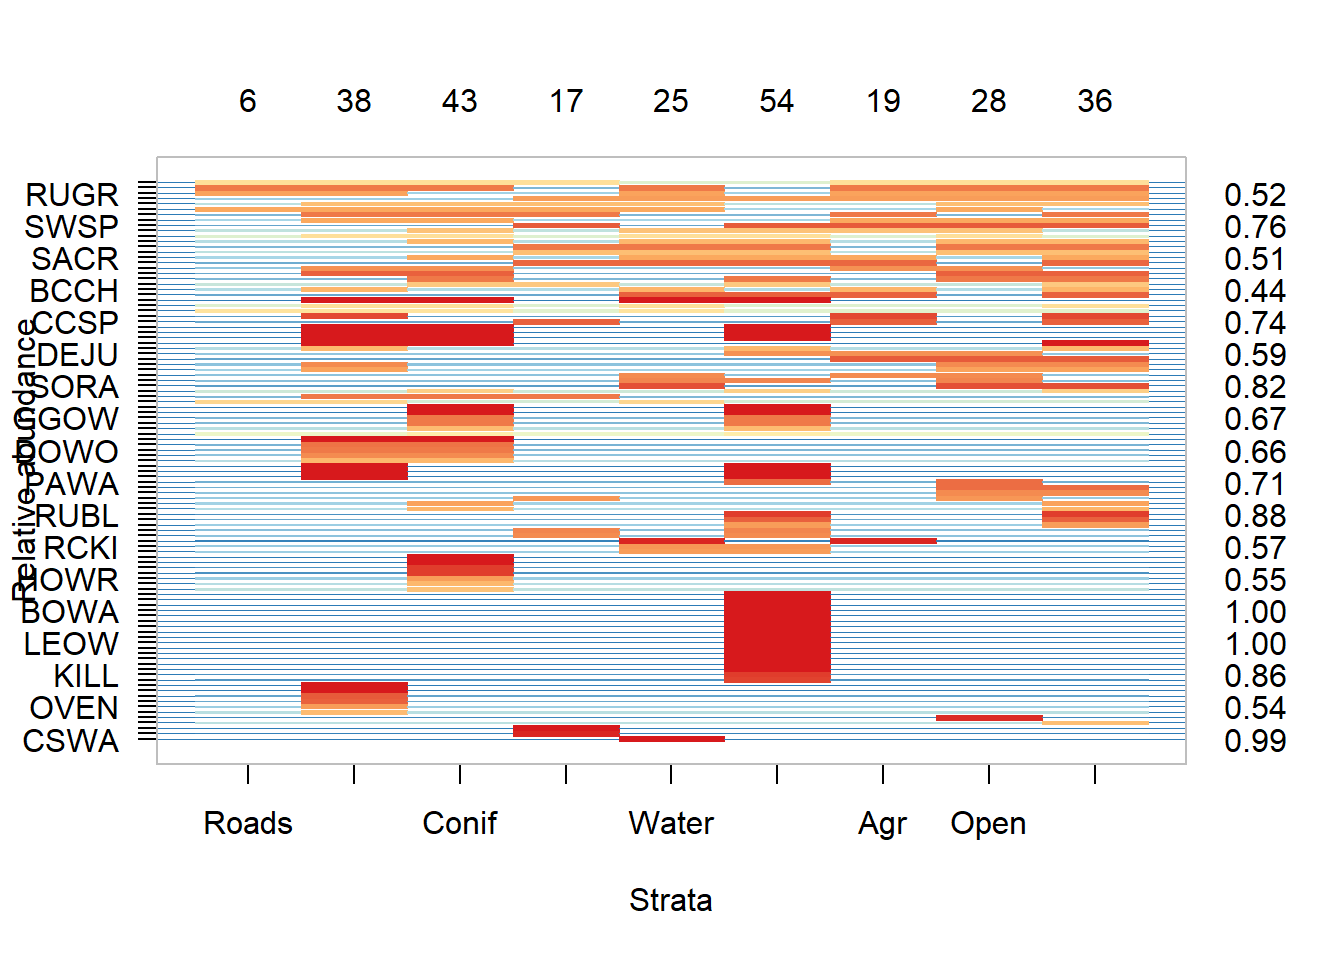
\includegraphics{qpad-book_files/figure-latex/unnamed-chunk-32-1.pdf}

\hypertarget{finding-optimal-combinations-of-factor-levels}{%
\subsection{Finding optimal combinations of factor levels}\label{finding-optimal-combinations-of-factor-levels}}

Categorical and compositional data

\begin{Shaded}
\begin{Highlighting}[]
\CommentTok{# dominant hab}
\NormalTok{M <-}\StringTok{ }\KeywordTok{model.matrix}\NormalTok{(}\OperatorTok{~}\NormalTok{hab}\DecValTok{-1}\NormalTok{, x)}
\KeywordTok{colnames}\NormalTok{(M) <-}\StringTok{ }\KeywordTok{levels}\NormalTok{(x}\OperatorTok{$}\NormalTok{hab)}
\NormalTok{ol1 <-}\StringTok{ }\KeywordTok{optilevels}\NormalTok{(x}\OperatorTok{$}\NormalTok{y, M, }\DataTypeTok{dist=}\StringTok{"poisson"}\NormalTok{)}
\KeywordTok{sort}\NormalTok{(}\KeywordTok{exp}\NormalTok{(}\KeywordTok{coef}\NormalTok{(}\KeywordTok{bestmodel}\NormalTok{(ol1))))}
\end{Highlighting}
\end{Shaded}

\begin{verbatim}
## `Open+UrbInd+Roads+OpenWet+ConifWet` 
##                               0.3366 
##                    `Water+Agr+Conif` 
##                               0.6232 
##                                Decid 
##                               1.4304
\end{verbatim}

\begin{Shaded}
\begin{Highlighting}[]
\CommentTok{## estimates}
\KeywordTok{exp}\NormalTok{(ol1}\OperatorTok{$}\NormalTok{coef)}
\end{Highlighting}
\end{Shaded}

\begin{verbatim}
##         Open  Water    Agr UrbInd      Roads Decid OpenWet
##  [1,] 0.2500 0.7000 0.5000 0.2857 0.00000454  1.43  0.3813
##  [2,] 0.2692 0.7000 0.5000 0.2692 0.00000454  1.43  0.3813
##  [3,] 0.2692 0.6238 0.5000 0.2692 0.00000454  1.43  0.3812
##  [4,] 0.2692 0.6232 0.6232 0.2692 0.00000454  1.43  0.3813
##  [5,] 0.3325 0.6232 0.6232 0.3325 0.00000454  1.43  0.3813
##  [6,] 0.3370 0.6232 0.6232 0.3370 0.00000454  1.43  0.3370
##  [7,] 0.3366 0.6232 0.6232 0.3366 0.33661645  1.43  0.3366
##  [8,]     NA     NA     NA     NA         NA    NA      NA
##  [9,]     NA     NA     NA     NA         NA    NA      NA
##        Conif ConifWet
##  [1,] 0.6228   0.3336
##  [2,] 0.6228   0.3336
##  [3,] 0.6238   0.3336
##  [4,] 0.6232   0.3336
##  [5,] 0.6232   0.3325
##  [6,] 0.6232   0.3370
##  [7,] 0.6232   0.3366
##  [8,]     NA       NA
##  [9,]     NA       NA
\end{verbatim}

\begin{Shaded}
\begin{Highlighting}[]
\CommentTok{## optimal classification}
\NormalTok{ol1}\OperatorTok{$}\NormalTok{rank}
\end{Highlighting}
\end{Shaded}

\begin{verbatim}
##       Open Water Agr UrbInd Roads Decid OpenWet Conif ConifWet
##  [1,]    2     8   6      3     1     9       5     7        4
##  [2,]    2     7   5      2     1     8       4     6        3
##  [3,]    2     6   5      2     1     7       4     6        3
##  [4,]    2     5   5      2     1     6       4     5        3
##  [5,]    2     4   4      2     1     5       3     4        2
##  [6,]    2     3   3      2     1     4       2     3        2
##  [7,]    1     2   2      1     1     3       1     2        1
##  [8,]   NA    NA  NA     NA    NA    NA      NA    NA       NA
##  [9,]   NA    NA  NA     NA    NA    NA      NA    NA       NA
\end{verbatim}

\begin{Shaded}
\begin{Highlighting}[]
\NormalTok{ol1}\OperatorTok{$}\NormalTok{levels[[}\KeywordTok{length}\NormalTok{(ol1}\OperatorTok{$}\NormalTok{levels)]]}
\end{Highlighting}
\end{Shaded}

\begin{verbatim}
##                                 Open 
## "Open+UrbInd+Roads+OpenWet+ConifWet" 
##                                Water 
##                    "Water+Agr+Conif" 
##                                  Agr 
##                    "Water+Agr+Conif" 
##                               UrbInd 
## "Open+UrbInd+Roads+OpenWet+ConifWet" 
##                                Roads 
## "Open+UrbInd+Roads+OpenWet+ConifWet" 
##                                Decid 
##                              "Decid" 
##                              OpenWet 
## "Open+UrbInd+Roads+OpenWet+ConifWet" 
##                                Conif 
##                    "Water+Agr+Conif" 
##                             ConifWet 
## "Open+UrbInd+Roads+OpenWet+ConifWet"
\end{verbatim}

\begin{Shaded}
\begin{Highlighting}[]
\CommentTok{# composition}
\NormalTok{ol2 <-}\StringTok{ }\KeywordTok{optilevels}\NormalTok{(x}\OperatorTok{$}\NormalTok{y, x[,cn], }\DataTypeTok{dist=}\StringTok{"poisson"}\NormalTok{)}
\KeywordTok{sort}\NormalTok{(}\KeywordTok{exp}\NormalTok{(}\KeywordTok{coef}\NormalTok{(}\KeywordTok{bestmodel}\NormalTok{(ol2))))}
\end{Highlighting}
\end{Shaded}

\begin{verbatim}
##                               Open 
##                            0.04936 
##                           ConifWet 
##                            0.18363 
## `Agr+UrbInd+SoftLin+OpenWet+Conif` 
##                            0.50444 
##                      `Water+Roads` 
##                            1.15427 
##                              Decid 
##                            2.49578
\end{verbatim}

\begin{Shaded}
\begin{Highlighting}[]
\CommentTok{## estimates}
\KeywordTok{exp}\NormalTok{(ol2}\OperatorTok{$}\NormalTok{coef)}
\end{Highlighting}
\end{Shaded}

\begin{verbatim}
##          Open Water    Agr UrbInd SoftLin Roads Decid OpenWet
##  [1,] 0.04790 1.174 0.5579 0.4313  0.5102 1.038 2.496  0.5627
##  [2,] 0.04791 1.174 0.5625 0.4313  0.5104 1.038 2.496  0.5625
##  [3,] 0.04795 1.174 0.5628 0.4324  0.4944 1.046 2.497  0.5628
##  [4,] 0.04790 1.156 0.5628 0.4291  0.4940 1.156 2.494  0.5628
##  [5,] 0.04782 1.146 0.5632 0.4917  0.4917 1.146 2.493  0.5632
##  [6,] 0.04936 1.154 0.5044 0.5044  0.5044 1.154 2.496  0.5044
##  [7,]      NA    NA     NA     NA      NA    NA    NA      NA
##  [8,]      NA    NA     NA     NA      NA    NA    NA      NA
##  [9,]      NA    NA     NA     NA      NA    NA    NA      NA
## [10,]      NA    NA     NA     NA      NA    NA    NA      NA
##        Conif ConifWet
##  [1,] 0.4941   0.1827
##  [2,] 0.4941   0.1827
##  [3,] 0.4944   0.1828
##  [4,] 0.4940   0.1828
##  [5,] 0.4917   0.1826
##  [6,] 0.5044   0.1836
##  [7,]     NA       NA
##  [8,]     NA       NA
##  [9,]     NA       NA
## [10,]     NA       NA
\end{verbatim}

\begin{Shaded}
\begin{Highlighting}[]
\CommentTok{## optimal classification}
\NormalTok{ol2}\OperatorTok{$}\NormalTok{rank}
\end{Highlighting}
\end{Shaded}

\begin{verbatim}
##       Open Water Agr UrbInd SoftLin Roads Decid OpenWet Conif
##  [1,]    1     9   6      3       5     8    10       7     4
##  [2,]    1     8   6      3       5     7     9       6     4
##  [3,]    1     7   5      3       4     6     8       5     4
##  [4,]    1     6   5      3       4     6     7       5     4
##  [5,]    1     5   4      3       3     5     6       4     3
##  [6,]    1     4   3      3       3     4     5       3     3
##  [7,]   NA    NA  NA     NA      NA    NA    NA      NA    NA
##  [8,]   NA    NA  NA     NA      NA    NA    NA      NA    NA
##  [9,]   NA    NA  NA     NA      NA    NA    NA      NA    NA
## [10,]   NA    NA  NA     NA      NA    NA    NA      NA    NA
##       ConifWet
##  [1,]        2
##  [2,]        2
##  [3,]        2
##  [4,]        2
##  [5,]        2
##  [6,]        2
##  [7,]       NA
##  [8,]       NA
##  [9,]       NA
## [10,]       NA
\end{verbatim}

\begin{Shaded}
\begin{Highlighting}[]
\KeywordTok{head}\NormalTok{(mefa4}\OperatorTok{::}\KeywordTok{groupSums}\NormalTok{(}\KeywordTok{as.matrix}\NormalTok{(x[,cn]), }\DecValTok{2}\NormalTok{, ol2}\OperatorTok{$}\NormalTok{levels[[}\KeywordTok{length}\NormalTok{(ol2}\OperatorTok{$}\NormalTok{levels)]]))}
\end{Highlighting}
\end{Shaded}

\begin{verbatim}
##         Open Water+Roads Agr+UrbInd+SoftLin+OpenWet+Conif
## CL10102    0    0.073010                          0.03326
## CL10106    0    0.008431                          0.60166
## CL10108    0    0.008431                          0.60166
## CL10109    0    0.036146                          0.08157
## CL10111    0    0.050734                          0.13353
## CL10112    0    0.050734                          0.13353
##           Decid ConifWet
## CL10102 0.85691 0.036819
## CL10106 0.04429 0.345625
## CL10108 0.04429 0.345625
## CL10109 0.88228 0.000000
## CL10111 0.81394 0.001797
## CL10112 0.81394 0.001797
\end{verbatim}

\hypertarget{interactions}{%
\section{Interactions}\label{interactions}}

\begin{Shaded}
\begin{Highlighting}[]
\NormalTok{mP4 <-}\StringTok{ }\KeywordTok{glm}\NormalTok{(y }\OperatorTok{~}\StringTok{ }\NormalTok{Decid }\OperatorTok{+}\StringTok{ }\NormalTok{ConifWet, }\DataTypeTok{data=}\NormalTok{x, }\DataTypeTok{family=}\NormalTok{poisson)}
\NormalTok{mP5 <-}\StringTok{ }\KeywordTok{glm}\NormalTok{(y }\OperatorTok{~}\StringTok{ }\NormalTok{Decid }\OperatorTok{*}\StringTok{ }\NormalTok{ConifWet, }\DataTypeTok{data=}\NormalTok{x, }\DataTypeTok{family=}\NormalTok{poisson)}
\KeywordTok{AIC}\NormalTok{(mP0, mP1, mP4, mP5)}
\KeywordTok{summary}\NormalTok{(mP5)}
\end{Highlighting}
\end{Shaded}

\begin{verbatim}
## 
## Call:
## glm(formula = y ~ Decid * ConifWet, family = poisson, data = x)
## 
## Deviance Residuals: 
##    Min      1Q  Median      3Q     Max  
## -2.081  -1.022  -0.484   0.374   4.321  
## 
## Coefficients:
##                Estimate Std. Error z value            Pr(>|z|)
## (Intercept)     -0.5604     0.0566    -9.9 <0.0000000000000002
## Decid            1.2125     0.0782    15.5 <0.0000000000000002
## ConifWet        -2.3124     0.1490   -15.5 <0.0000000000000002
## Decid:ConifWet   5.3461     0.3566    15.0 <0.0000000000000002
##                   
## (Intercept)    ***
## Decid          ***
## ConifWet       ***
## Decid:ConifWet ***
## ---
## Signif. codes:  0 '***' 0.001 '**' 0.01 '*' 0.05 '.' 0.1 ' ' 1
## 
## (Dispersion parameter for poisson family taken to be 1)
## 
##     Null deviance: 7424.8  on 4568  degrees of freedom
## Residual deviance: 5395.2  on 4565  degrees of freedom
## AIC: 10549
## 
## Number of Fisher Scoring iterations: 6
\end{verbatim}

\begin{Shaded}
\begin{Highlighting}[]
\KeywordTok{visreg}\NormalTok{(mGAM, }\DataTypeTok{scale=}\StringTok{"response"}\NormalTok{)}
\end{Highlighting}
\end{Shaded}

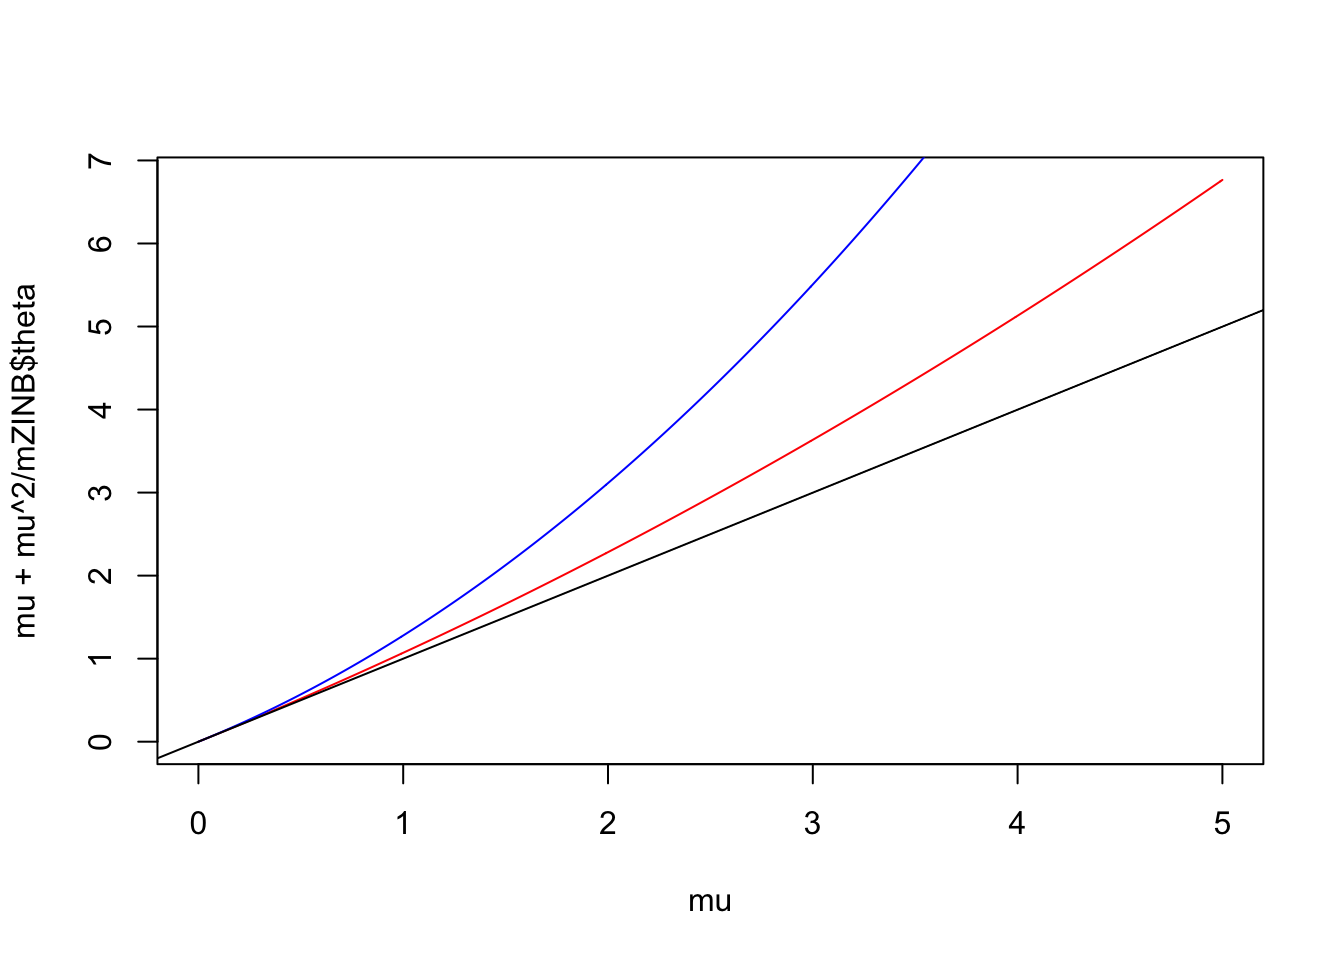
\includegraphics{qpad-book_files/figure-latex/unnamed-chunk-34-1.pdf}

\begin{Shaded}
\begin{Highlighting}[]
\KeywordTok{visreg}\NormalTok{(mP1, }\DataTypeTok{scale=}\StringTok{"response"}\NormalTok{)}
\end{Highlighting}
\end{Shaded}

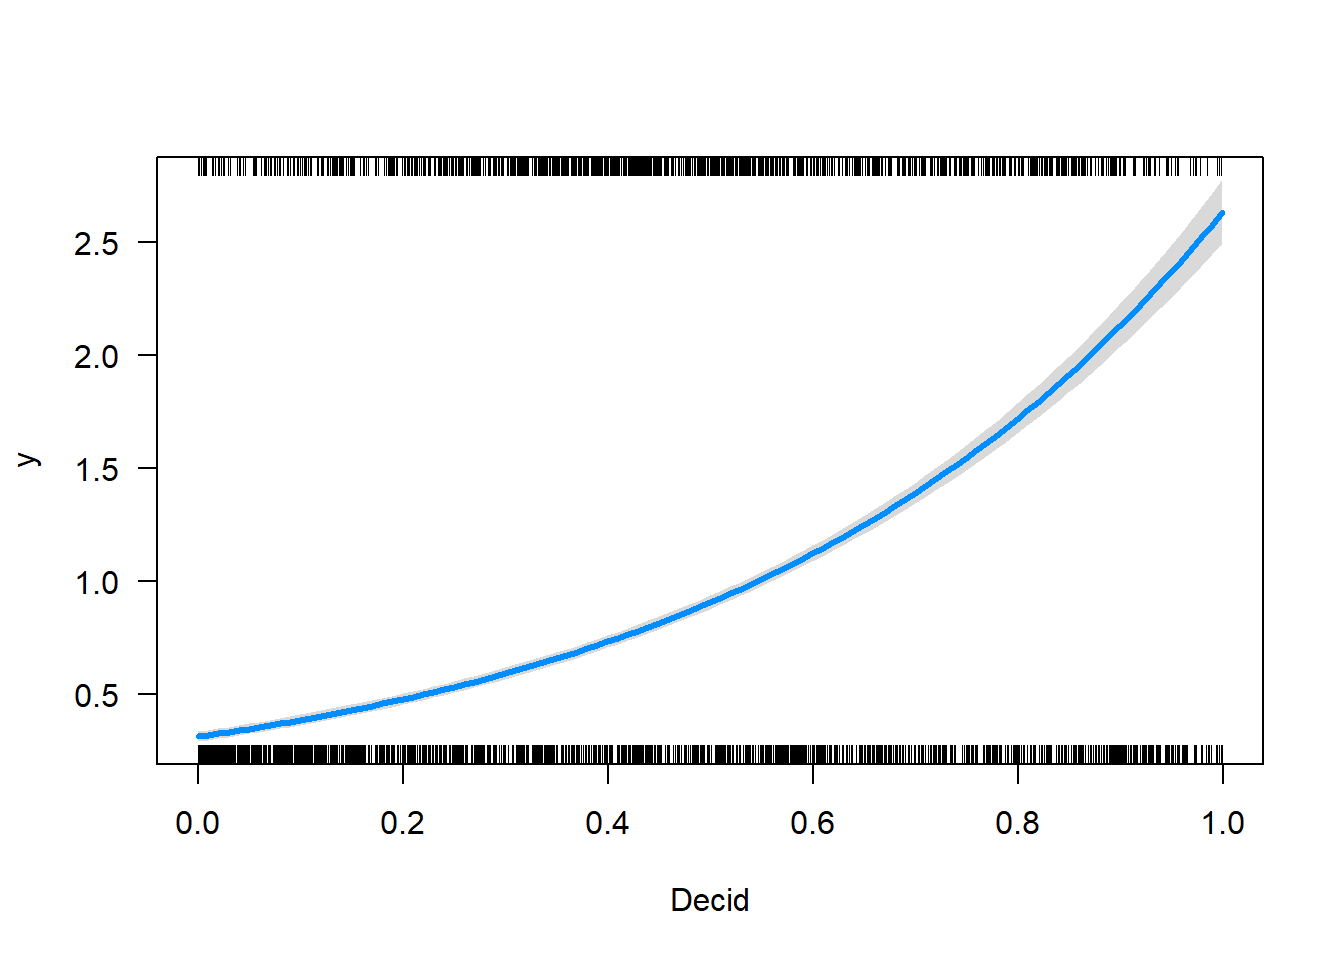
\includegraphics{qpad-book_files/figure-latex/unnamed-chunk-34-2.pdf}

\begin{Shaded}
\begin{Highlighting}[]
\KeywordTok{visreg}\NormalTok{(mP4, }\DataTypeTok{scale=}\StringTok{"response"}\NormalTok{)}
\end{Highlighting}
\end{Shaded}

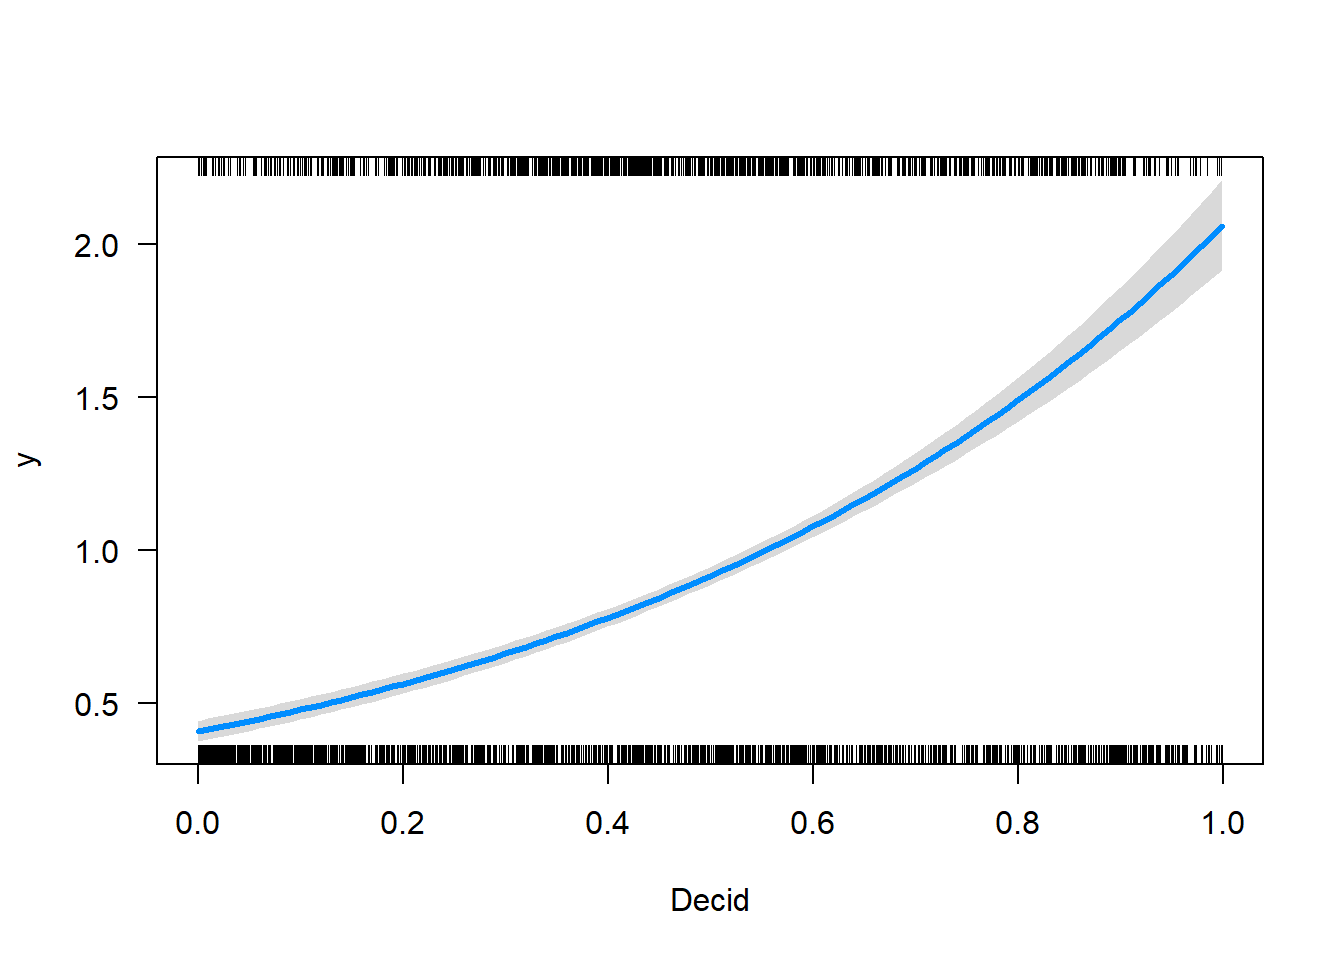
\includegraphics{qpad-book_files/figure-latex/unnamed-chunk-34-3.pdf} 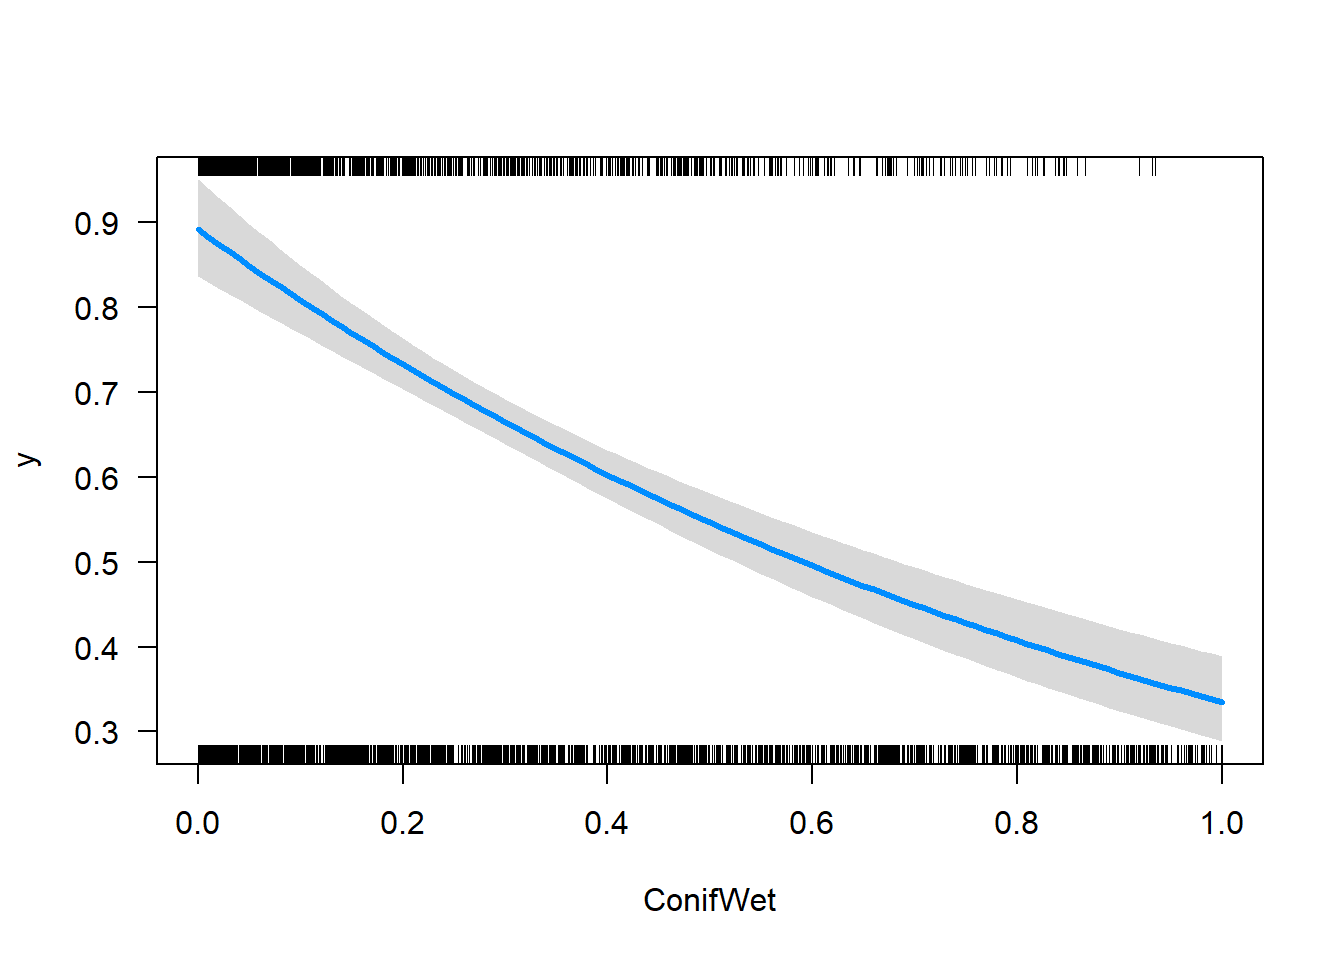
\includegraphics{qpad-book_files/figure-latex/unnamed-chunk-34-4.pdf}

\begin{Shaded}
\begin{Highlighting}[]
\KeywordTok{visreg}\NormalTok{(mP5, }\DataTypeTok{scale=}\StringTok{"response"}\NormalTok{, }\DataTypeTok{xvar=}\StringTok{"Decid"}\NormalTok{, }\DataTypeTok{by=}\StringTok{"ConifWet"}\NormalTok{)}
\end{Highlighting}
\end{Shaded}

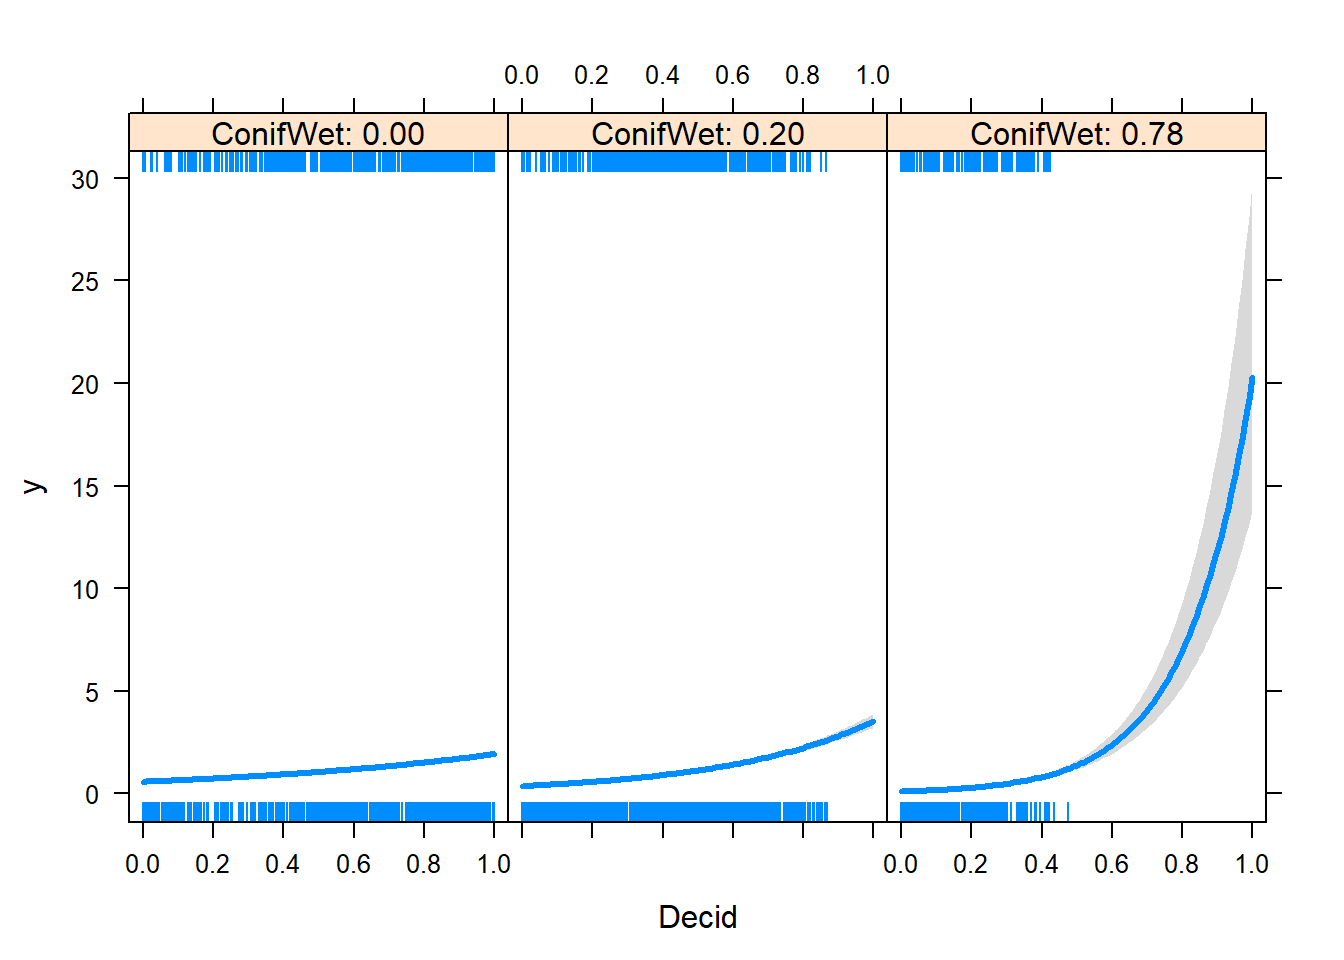
\includegraphics{qpad-book_files/figure-latex/unnamed-chunk-34-5.pdf}

\begin{Shaded}
\begin{Highlighting}[]
\KeywordTok{round}\NormalTok{(}\KeywordTok{rbind}\NormalTok{(}\DataTypeTok{mP0=}\KeywordTok{R2dev}\NormalTok{(mP0), }\DataTypeTok{mP1=}\KeywordTok{R2dev}\NormalTok{(mP1), }\DataTypeTok{mP2=}\KeywordTok{R2dev}\NormalTok{(mP2), }\DataTypeTok{mP3=}\KeywordTok{R2dev}\NormalTok{(mP3),}
  \DataTypeTok{mP4=}\KeywordTok{R2dev}\NormalTok{(mP4), }\DataTypeTok{mP5=}\KeywordTok{R2dev}\NormalTok{(mP5)), }\DecValTok{4}\NormalTok{)}
\end{Highlighting}
\end{Shaded}

\begin{verbatim}
##         R2  R2adj Deviance Dev0 DevR  df0  dfR p_value
## mP0 0.0000 0.0000        0 7425 7425 4568 4568       0
## mP1 0.2273 0.2272     1688 7425 5737 4568 4567       0
## mP2 0.2591 0.2575     1924 7425 5501 4568 4558       0
## mP3 0.1923 0.1909     1428 7425 5997 4568 4560       0
## mP4 0.2406 0.2403     1786 7425 5638 4568 4566       0
## mP5 0.2734 0.2729     2030 7425 5395 4568 4565       0
\end{verbatim}

\begin{Shaded}
\begin{Highlighting}[]
\KeywordTok{model.sel}\NormalTok{(mP0, mP1, mP2, mP3, mP4, mP5)}
\end{Highlighting}
\end{Shaded}

\begin{verbatim}
## Model selection table 
##       (Int)    Dcd     Cnf     CnW   DAY    Ltt     Lng    Opn
## mP5 -0.5604 1.2130         -2.3120                            
## mP2 -5.8830 0.8337 -0.8856 -1.8940 -2.88 0.2093 0.03831 -3.474
## mP4 -0.7014 1.6220         -0.9785                            
## mP1 -1.1640 2.1340                                            
## mP3 -1.3860                                                   
## mP0 -0.1243                                                   
##         OpW    TSS    UrI hab CnW:Dcd df logLik  AICc  delta
## mP5                             5.346  4  -5271 10549    0.0
## mP2 -0.7408 -1.234 -1.669             11  -5324 10669  120.0
## mP4                                    3  -5392 10791  241.2
## mP1                                    2  -5442 10887  337.7
## mP3                         +          9  -5572 11162  612.1
## mP0                                    1  -6285 12573 2023.6
##     weight
## mP5      1
## mP2      0
## mP4      0
## mP1      0
## mP3      0
## mP0      0
## Models ranked by AICc(x)
\end{verbatim}

\hypertarget{different-error-distributions}{%
\section{Different error distributions}\label{different-error-distributions}}

\begin{Shaded}
\begin{Highlighting}[]
\NormalTok{mP <-}\StringTok{ }\NormalTok{mP5 }\CommentTok{# best Poisson}
\NormalTok{mNB <-}\StringTok{ }\KeywordTok{glm.nb}\NormalTok{(y }\OperatorTok{~}\StringTok{ }\NormalTok{Decid }\OperatorTok{*}\StringTok{ }\NormalTok{ConifWet, }\DataTypeTok{data=}\NormalTok{x)}
\NormalTok{mZIP <-}\StringTok{ }\KeywordTok{zeroinfl}\NormalTok{(y }\OperatorTok{~}\StringTok{ }\NormalTok{Decid }\OperatorTok{*}\StringTok{ }\NormalTok{ConifWet }\OperatorTok{|}\StringTok{ }\DecValTok{1}\NormalTok{, x, }\DataTypeTok{dist=}\StringTok{"poisson"}\NormalTok{)}
\NormalTok{mZINB <-}\StringTok{ }\KeywordTok{zeroinfl}\NormalTok{(y }\OperatorTok{~}\StringTok{ }\NormalTok{Decid }\OperatorTok{*}\StringTok{ }\NormalTok{ConifWet }\OperatorTok{|}\StringTok{ }\DecValTok{1}\NormalTok{, x, }\DataTypeTok{dist=}\StringTok{"negbin"}\NormalTok{)}

\KeywordTok{AIC}\NormalTok{(mP, mNB, mZIP, mZINB)}
\KeywordTok{summary}\NormalTok{(mZINB)}
\end{Highlighting}
\end{Shaded}

\begin{verbatim}
## 
## Call:
## zeroinfl(formula = y ~ Decid * ConifWet | 1, data = x, dist = "negbin")
## 
## Pearson residuals:
##    Min     1Q Median     3Q    Max 
## -1.190 -0.689 -0.338  0.361  8.956 
## 
## Count model coefficients (negbin with log link):
##                Estimate Std. Error z value             Pr(>|z|)
## (Intercept)     -0.3873     0.0732   -5.29           0.00000012
## Decid            1.1195     0.0911   12.29 < 0.0000000000000002
## ConifWet        -2.4230     0.1589  -15.25 < 0.0000000000000002
## Decid:ConifWet   5.9227     0.3963   14.94 < 0.0000000000000002
## Log(theta)       2.6504     0.5305    5.00           0.00000059
##                   
## (Intercept)    ***
## Decid          ***
## ConifWet       ***
## Decid:ConifWet ***
## Log(theta)     ***
## 
## Zero-inflation model coefficients (binomial with logit link):
##             Estimate Std. Error z value            Pr(>|z|)    
## (Intercept)   -1.861      0.193   -9.64 <0.0000000000000002 ***
## ---
## Signif. codes:  0 '***' 0.001 '**' 0.01 '*' 0.05 '.' 0.1 ' ' 1 
## 
## Theta = 14.159 
## Number of iterations in BFGS optimization: 22 
## Log-likelihood: -5.2e+03 on 6 Df
\end{verbatim}

\begin{Shaded}
\begin{Highlighting}[]
\KeywordTok{plogis}\NormalTok{(}\KeywordTok{coef}\NormalTok{(mZINB, }\StringTok{"zero"}\NormalTok{)) }\CommentTok{# P of 0}
\end{Highlighting}
\end{Shaded}

\begin{verbatim}
## (Intercept) 
##      0.1346
\end{verbatim}

\begin{Shaded}
\begin{Highlighting}[]
\NormalTok{mZINB}\OperatorTok{$}\NormalTok{theta }\CommentTok{# V(mu) = mu + mu^2/theta, ~inverse of variance}
\end{Highlighting}
\end{Shaded}

\begin{verbatim}
## [1] 14.16
\end{verbatim}

\begin{Shaded}
\begin{Highlighting}[]
\CommentTok{# Variance function, 1:1 is Poisson}
\NormalTok{mu <-}\StringTok{ }\KeywordTok{seq}\NormalTok{(}\DecValTok{0}\NormalTok{, }\DecValTok{5}\NormalTok{, }\FloatTok{0.01}\NormalTok{)}
\NormalTok{theta <-}\StringTok{ }\NormalTok{mZINB}\OperatorTok{$}\NormalTok{theta}
\KeywordTok{plot}\NormalTok{(mu, mu }\OperatorTok{+}\StringTok{ }\NormalTok{mu}\OperatorTok{^}\DecValTok{2}\OperatorTok{/}\NormalTok{mZINB}\OperatorTok{$}\NormalTok{theta, }\DataTypeTok{type=}\StringTok{"l"}\NormalTok{, }\DataTypeTok{col=}\DecValTok{2}\NormalTok{)}
\KeywordTok{lines}\NormalTok{(mu, mu }\OperatorTok{+}\StringTok{ }\NormalTok{mu}\OperatorTok{^}\DecValTok{2}\OperatorTok{/}\NormalTok{mNB}\OperatorTok{$}\NormalTok{theta, }\DataTypeTok{type=}\StringTok{"l"}\NormalTok{, }\DataTypeTok{col=}\DecValTok{4}\NormalTok{)}
\KeywordTok{abline}\NormalTok{(}\DecValTok{0}\NormalTok{,}\DecValTok{1}\NormalTok{)}
\end{Highlighting}
\end{Shaded}

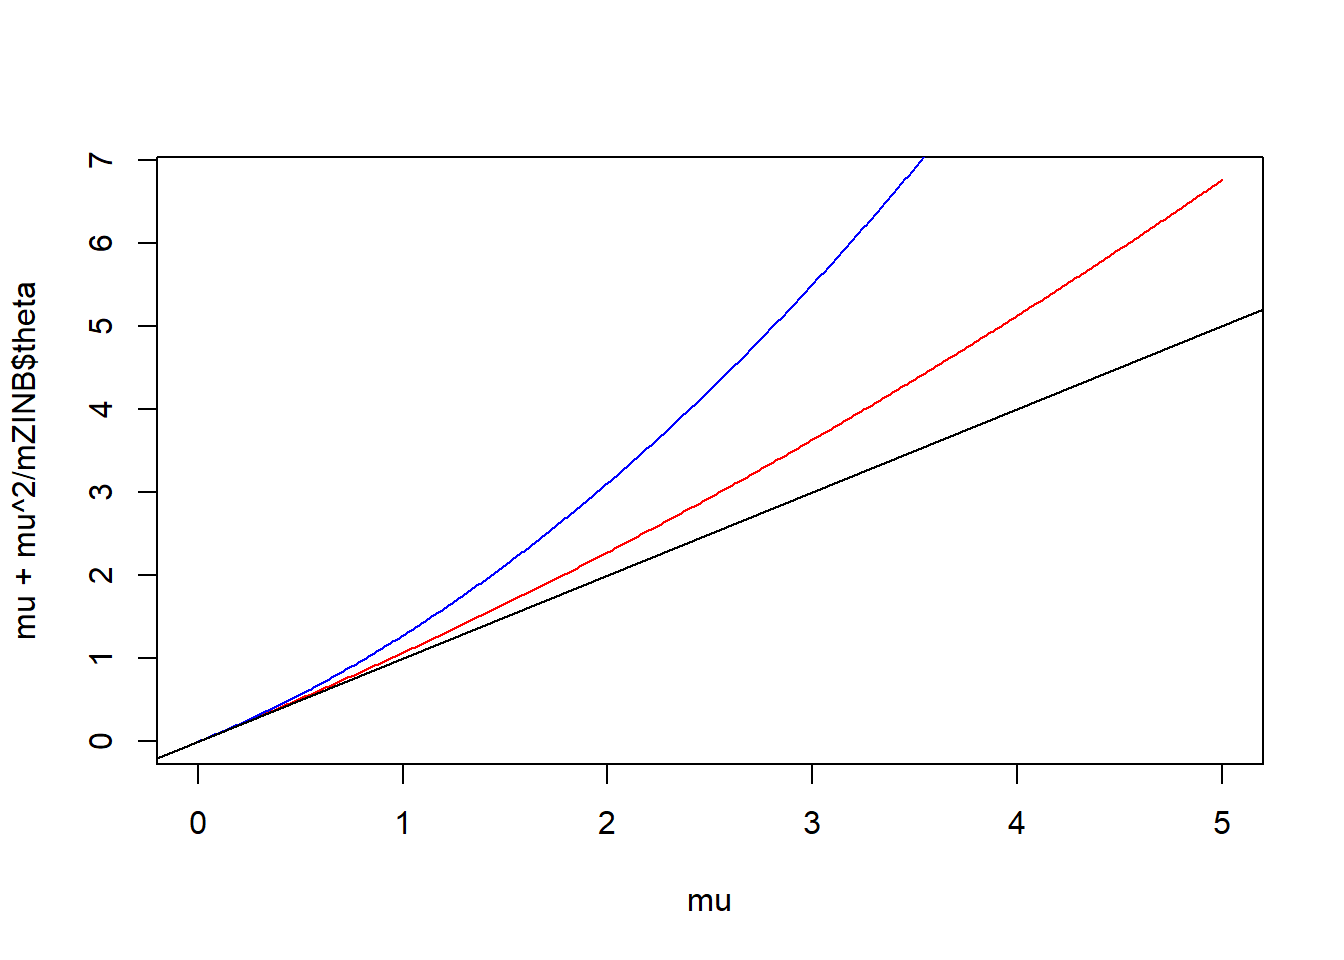
\includegraphics{qpad-book_files/figure-latex/unnamed-chunk-35-1.pdf}

Poisson-Lognormal random effects, iid. and clustered:

\begin{Shaded}
\begin{Highlighting}[]
\NormalTok{mPLN1 <-}\StringTok{ }\KeywordTok{glmer}\NormalTok{(y }\OperatorTok{~}\StringTok{ }\NormalTok{Decid }\OperatorTok{*}\StringTok{ }\NormalTok{ConifWet }\OperatorTok{+}\StringTok{ }\NormalTok{(}\DecValTok{1} \OperatorTok{|}\StringTok{ }\NormalTok{SiteID), }\DataTypeTok{data=}\NormalTok{x, }\DataTypeTok{family=}\NormalTok{poisson)}
\NormalTok{mPLN2 <-}\StringTok{ }\KeywordTok{glmer}\NormalTok{(y }\OperatorTok{~}\StringTok{ }\NormalTok{Decid }\OperatorTok{*}\StringTok{ }\NormalTok{ConifWet }\OperatorTok{+}\StringTok{ }\NormalTok{(}\DecValTok{1} \OperatorTok{|}\StringTok{ }\NormalTok{SurveyArea), }\DataTypeTok{data=}\NormalTok{x, }\DataTypeTok{family=}\NormalTok{poisson)}
\KeywordTok{AIC}\NormalTok{(mP, mNB, mZIP, mZINB, mPLN1, mPLN2)}
\KeywordTok{summary}\NormalTok{(mPLN2)}
\end{Highlighting}
\end{Shaded}

\begin{verbatim}
## Generalized linear mixed model fit by maximum likelihood
##   (Laplace Approximation) [glmerMod]
##  Family: poisson  ( log )
## Formula: y ~ Decid * ConifWet + (1 | SurveyArea)
##    Data: x
## 
##      AIC      BIC   logLik deviance df.resid 
##    10021    10053    -5006    10011     4564 
## 
## Scaled residuals: 
##    Min     1Q Median     3Q    Max 
## -1.739 -0.643 -0.320  0.355  6.535 
## 
## Random effects:
##  Groups     Name        Variance Std.Dev.
##  SurveyArea (Intercept) 0.295    0.543   
## Number of obs: 4569, groups:  SurveyArea, 271
## 
## Fixed effects:
##                Estimate Std. Error z value            Pr(>|z|)
## (Intercept)     -0.7459     0.0783   -9.53 <0.0000000000000002
## Decid            1.1967     0.0984   12.16 <0.0000000000000002
## ConifWet        -2.3213     0.1687  -13.76 <0.0000000000000002
## Decid:ConifWet   5.5346     0.3978   13.91 <0.0000000000000002
##                   
## (Intercept)    ***
## Decid          ***
## ConifWet       ***
## Decid:ConifWet ***
## ---
## Signif. codes:  0 '***' 0.001 '**' 0.01 '*' 0.05 '.' 0.1 ' ' 1
## 
## Correlation of Fixed Effects:
##             (Intr) Decid  ConfWt
## Decid       -0.808              
## ConifWet    -0.610  0.628       
## Decid:CnfWt  0.162 -0.325 -0.670
\end{verbatim}

\hypertarget{counting-time-effects}{%
\section{Counting time effects}\label{counting-time-effects}}

\begin{Shaded}
\begin{Highlighting}[]
\NormalTok{spp <-}\StringTok{ "OVEN"} \CommentTok{# which species}

\NormalTok{ydur <-}\StringTok{ }\KeywordTok{Xtab}\NormalTok{(}\OperatorTok{~}\StringTok{ }\NormalTok{SiteID }\OperatorTok{+}\StringTok{ }\NormalTok{Dur }\OperatorTok{+}\StringTok{ }\NormalTok{SpeciesID , josm}\OperatorTok{$}\NormalTok{counts[josm}\OperatorTok{$}\NormalTok{counts}\OperatorTok{$}\NormalTok{DetectType1 }\OperatorTok{!=}\StringTok{ "V"}\NormalTok{,])}

\NormalTok{y <-}\StringTok{ }\KeywordTok{as.matrix}\NormalTok{(ydur[[spp]])}
\KeywordTok{head}\NormalTok{(y)}
\end{Highlighting}
\end{Shaded}

\begin{verbatim}
##         0-3min 3-5min 5-10min
## CL10102      3      0       0
## CL10106      0      0       0
## CL10108      0      0       0
## CL10109      2      0       1
## CL10111      2      0       0
## CL10112      2      0       0
\end{verbatim}

\begin{Shaded}
\begin{Highlighting}[]
\KeywordTok{colMeans}\NormalTok{(y)}
\end{Highlighting}
\end{Shaded}

\begin{verbatim}
##  0-3min  3-5min 5-10min 
## 0.67367 0.09346 0.11600
\end{verbatim}

\begin{Shaded}
\begin{Highlighting}[]
\KeywordTok{cumsum}\NormalTok{(}\KeywordTok{colMeans}\NormalTok{(y))}
\end{Highlighting}
\end{Shaded}

\begin{verbatim}
##  0-3min  3-5min 5-10min 
##  0.6737  0.7671  0.8831
\end{verbatim}

\begin{Shaded}
\begin{Highlighting}[]
\NormalTok{x <-}\StringTok{ }\KeywordTok{data.frame}\NormalTok{(}
\NormalTok{  josm}\OperatorTok{$}\NormalTok{surveys, }
  \DataTypeTok{y3=}\NormalTok{y[,}\StringTok{"0-3min"}\NormalTok{],}
  \DataTypeTok{y5=}\NormalTok{y[,}\StringTok{"0-3min"}\NormalTok{]}\OperatorTok{+}\NormalTok{y[,}\StringTok{"3-5min"}\NormalTok{],}
  \DataTypeTok{y10=}\KeywordTok{rowSums}\NormalTok{(y))}

\KeywordTok{table}\NormalTok{(x}\OperatorTok{$}\NormalTok{y3)}
\end{Highlighting}
\end{Shaded}

\begin{verbatim}
## 
##    0    1    2    3    4    5    6 
## 2768  922  576  226   61   14    2
\end{verbatim}

\begin{Shaded}
\begin{Highlighting}[]
\KeywordTok{table}\NormalTok{(x}\OperatorTok{$}\NormalTok{y5)}
\end{Highlighting}
\end{Shaded}

\begin{verbatim}
## 
##    0    1    2    3    4    5    6 
## 2643  894  632  285   87   24    4
\end{verbatim}

\begin{Shaded}
\begin{Highlighting}[]
\KeywordTok{table}\NormalTok{(x}\OperatorTok{$}\NormalTok{y10)}
\end{Highlighting}
\end{Shaded}

\begin{verbatim}
## 
##    0    1    2    3    4    5    6 
## 2493  883  656  363  132   29   13
\end{verbatim}

\begin{Shaded}
\begin{Highlighting}[]
\NormalTok{m3 <-}\StringTok{ }\KeywordTok{glm}\NormalTok{(y3 }\OperatorTok{~}\StringTok{ }\NormalTok{Decid, }\DataTypeTok{data=}\NormalTok{x, }\DataTypeTok{family=}\NormalTok{poisson)}
\NormalTok{m5 <-}\StringTok{ }\KeywordTok{glm}\NormalTok{(y5 }\OperatorTok{~}\StringTok{ }\NormalTok{Decid, }\DataTypeTok{data=}\NormalTok{x, }\DataTypeTok{family=}\NormalTok{poisson)}
\NormalTok{m10 <-}\StringTok{ }\KeywordTok{glm}\NormalTok{(y10 }\OperatorTok{~}\StringTok{ }\NormalTok{Decid, }\DataTypeTok{data=}\NormalTok{x, }\DataTypeTok{family=}\NormalTok{poisson)}
\KeywordTok{mean}\NormalTok{(}\KeywordTok{fitted}\NormalTok{(m3))}
\end{Highlighting}
\end{Shaded}

\begin{verbatim}
## [1] 0.6737
\end{verbatim}

\begin{Shaded}
\begin{Highlighting}[]
\KeywordTok{mean}\NormalTok{(}\KeywordTok{fitted}\NormalTok{(m5))}
\end{Highlighting}
\end{Shaded}

\begin{verbatim}
## [1] 0.7671
\end{verbatim}

\begin{Shaded}
\begin{Highlighting}[]
\KeywordTok{mean}\NormalTok{(}\KeywordTok{fitted}\NormalTok{(m10))}
\end{Highlighting}
\end{Shaded}

\begin{verbatim}
## [1] 0.8831
\end{verbatim}

\begin{Shaded}
\begin{Highlighting}[]
\KeywordTok{set.seed}\NormalTok{(}\DecValTok{1}\NormalTok{)}
\NormalTok{x}\OperatorTok{$}\NormalTok{meth <-}\StringTok{ }\KeywordTok{sample}\NormalTok{(}\KeywordTok{c}\NormalTok{(}\StringTok{"A"}\NormalTok{, }\StringTok{"B"}\NormalTok{, }\StringTok{"C"}\NormalTok{), }\KeywordTok{nrow}\NormalTok{(x), }\DataTypeTok{replace=}\OtherTok{TRUE}\NormalTok{)}
\NormalTok{x}\OperatorTok{$}\NormalTok{y <-}\StringTok{ }\NormalTok{x}\OperatorTok{$}\NormalTok{y3}
\NormalTok{x}\OperatorTok{$}\NormalTok{y[x}\OperatorTok{$}\NormalTok{meth }\OperatorTok{==}\StringTok{ "B"}\NormalTok{] <-}\StringTok{ }\NormalTok{x}\OperatorTok{$}\NormalTok{y5[x}\OperatorTok{$}\NormalTok{meth }\OperatorTok{==}\StringTok{ "B"}\NormalTok{]}
\NormalTok{x}\OperatorTok{$}\NormalTok{y[x}\OperatorTok{$}\NormalTok{meth }\OperatorTok{==}\StringTok{ "C"}\NormalTok{] <-}\StringTok{ }\NormalTok{x}\OperatorTok{$}\NormalTok{y10[x}\OperatorTok{$}\NormalTok{meth }\OperatorTok{==}\StringTok{ "C"}\NormalTok{]}
\KeywordTok{boxplot}\NormalTok{(y }\OperatorTok{~}\StringTok{ }\NormalTok{meth, x)}
\end{Highlighting}
\end{Shaded}

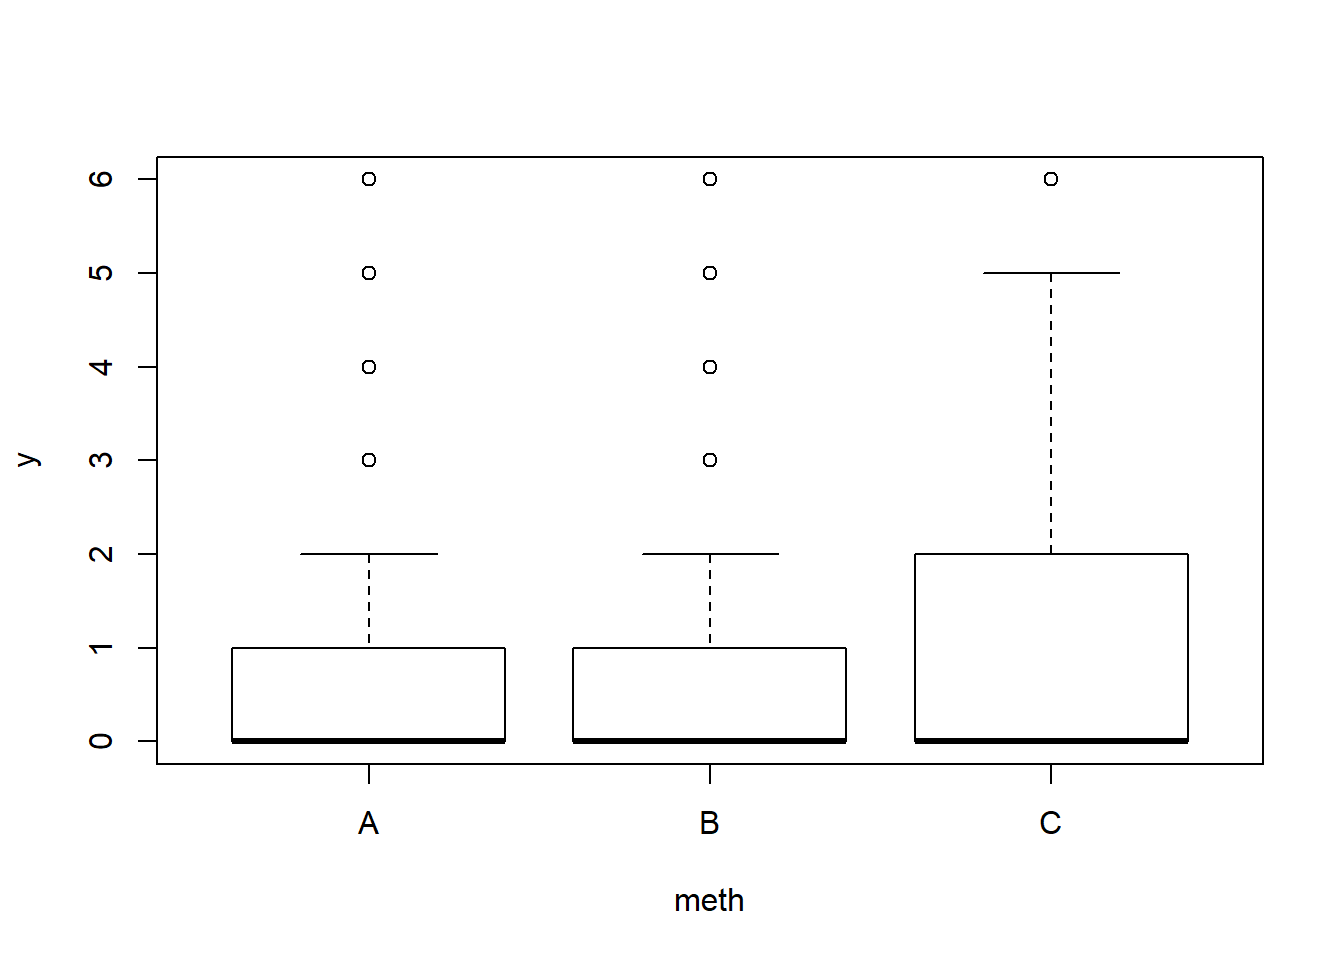
\includegraphics{qpad-book_files/figure-latex/unnamed-chunk-37-1.pdf}

\begin{Shaded}
\begin{Highlighting}[]
\NormalTok{mm <-}\StringTok{ }\KeywordTok{glm}\NormalTok{(y }\OperatorTok{~}\StringTok{ }\NormalTok{meth }\OperatorTok{-}\StringTok{ }\DecValTok{1}\NormalTok{, }\DataTypeTok{data=}\NormalTok{x, }\DataTypeTok{family=}\NormalTok{poisson)}
\KeywordTok{summary}\NormalTok{(mm)}
\end{Highlighting}
\end{Shaded}

\begin{verbatim}
## 
## Call:
## glm(formula = y ~ meth - 1, family = poisson, data = x)
## 
## Deviance Residuals: 
##    Min      1Q  Median      3Q     Max  
## -1.312  -1.273  -1.147   0.391   3.980  
## 
## Coefficients:
##       Estimate Std. Error z value             Pr(>|z|)    
## methA  -0.4186     0.0314  -13.32 < 0.0000000000000002 ***
## methB  -0.2100     0.0282   -7.44      0.0000000000001 ***
## methC  -0.1502     0.0280   -5.37      0.0000000794370 ***
## ---
## Signif. codes:  0 '***' 0.001 '**' 0.01 '*' 0.05 '.' 0.1 ' ' 1
## 
## (Dispersion parameter for poisson family taken to be 1)
## 
##     Null deviance: 7233.2  on 4569  degrees of freedom
## Residual deviance: 6938.6  on 4566  degrees of freedom
## AIC: 11646
## 
## Number of Fisher Scoring iterations: 6
\end{verbatim}

\begin{Shaded}
\begin{Highlighting}[]
\KeywordTok{exp}\NormalTok{(}\KeywordTok{coef}\NormalTok{(mm))}
\end{Highlighting}
\end{Shaded}

\begin{verbatim}
##  methA  methB  methC 
## 0.6580 0.8106 0.8605
\end{verbatim}

\begin{Shaded}
\begin{Highlighting}[]
\NormalTok{mm <-}\StringTok{ }\KeywordTok{glm}\NormalTok{(y }\OperatorTok{~}\StringTok{ }\NormalTok{Decid }\OperatorTok{+}\StringTok{ }\NormalTok{meth, }\DataTypeTok{data=}\NormalTok{x, }\DataTypeTok{family=}\NormalTok{poisson)}
\KeywordTok{summary}\NormalTok{(mm)}
\end{Highlighting}
\end{Shaded}

\begin{verbatim}
## 
## Call:
## glm(formula = y ~ Decid + meth, family = poisson, data = x)
## 
## Deviance Residuals: 
##    Min      1Q  Median      3Q     Max  
## -2.279  -0.953  -0.740   0.447   4.568  
## 
## Coefficients:
##             Estimate Std. Error z value             Pr(>|z|)    
## (Intercept)  -1.4616     0.0460  -31.80 < 0.0000000000000002 ***
## Decid         2.1450     0.0573   37.41 < 0.0000000000000002 ***
## methB         0.1669     0.0423    3.95     0.00007896414416 ***
## methC         0.3027     0.0421    7.19     0.00000000000064 ***
## ---
## Signif. codes:  0 '***' 0.001 '**' 0.01 '*' 0.05 '.' 0.1 ' ' 1
## 
## (Dispersion parameter for poisson family taken to be 1)
## 
##     Null deviance: 6983.3  on 4568  degrees of freedom
## Residual deviance: 5443.8  on 4565  degrees of freedom
## AIC: 10153
## 
## Number of Fisher Scoring iterations: 6
\end{verbatim}

\begin{Shaded}
\begin{Highlighting}[]
\KeywordTok{boxplot}\NormalTok{(}\KeywordTok{fitted}\NormalTok{(mm) }\OperatorTok{~}\StringTok{ }\NormalTok{meth, x)}
\end{Highlighting}
\end{Shaded}

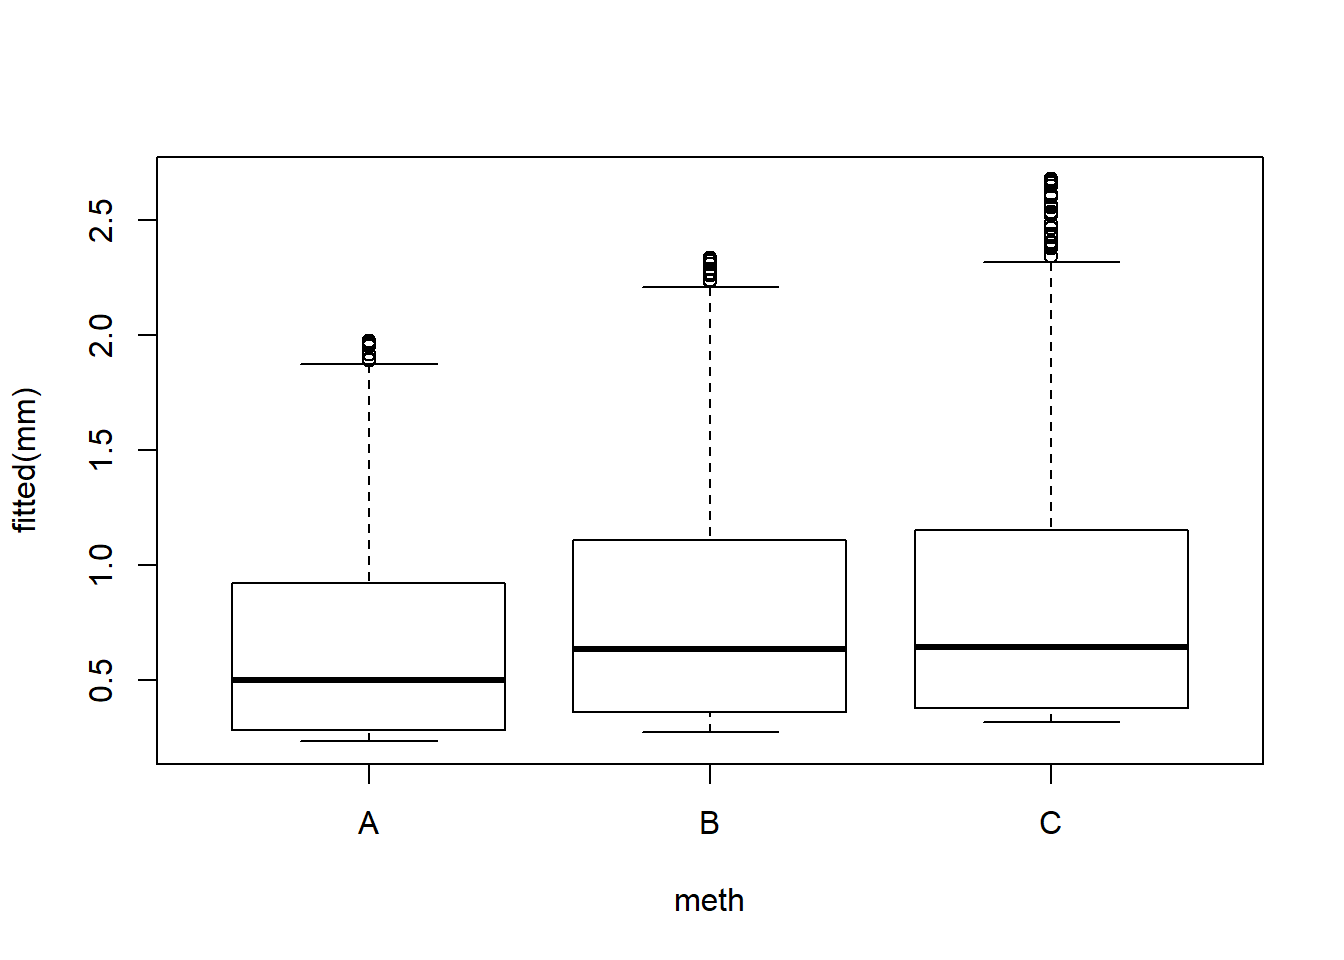
\includegraphics{qpad-book_files/figure-latex/unnamed-chunk-37-2.pdf}

\begin{Shaded}
\begin{Highlighting}[]
\KeywordTok{exp}\NormalTok{(}\KeywordTok{coef}\NormalTok{(mm))}
\end{Highlighting}
\end{Shaded}

\begin{verbatim}
## (Intercept)       Decid       methB       methC 
##      0.2319      8.5421      1.1816      1.3535
\end{verbatim}

\begin{Shaded}
\begin{Highlighting}[]
\KeywordTok{cumsum}\NormalTok{(}\KeywordTok{colMeans}\NormalTok{(y))}
\end{Highlighting}
\end{Shaded}

\begin{verbatim}
##  0-3min  3-5min 5-10min 
##  0.6737  0.7671  0.8831
\end{verbatim}

\begin{Shaded}
\begin{Highlighting}[]
\KeywordTok{mean}\NormalTok{(y[,}\DecValTok{1}\NormalTok{]) }\OperatorTok{*}\StringTok{ }\KeywordTok{c}\NormalTok{(}\DecValTok{1}\NormalTok{, }\KeywordTok{exp}\NormalTok{(}\KeywordTok{coef}\NormalTok{(mm))[}\DecValTok{3}\OperatorTok{:}\DecValTok{4}\NormalTok{])}
\end{Highlighting}
\end{Shaded}

\begin{verbatim}
##         methB  methC 
## 0.6737 0.7960 0.9118
\end{verbatim}

It is all relative, depends on reference methodology/protocol.

\hypertarget{counting-radius-effects}{%
\section{Counting radius effects}\label{counting-radius-effects}}

Use area subsets to demonstrate use of offsets

\begin{Shaded}
\begin{Highlighting}[]
\NormalTok{spp <-}\StringTok{ "OVEN"} \CommentTok{# which species}

\NormalTok{ydis <-}\StringTok{ }\KeywordTok{Xtab}\NormalTok{(}\OperatorTok{~}\StringTok{ }\NormalTok{SiteID }\OperatorTok{+}\StringTok{ }\NormalTok{Dis }\OperatorTok{+}\StringTok{ }\NormalTok{SpeciesID , josm}\OperatorTok{$}\NormalTok{counts[josm}\OperatorTok{$}\NormalTok{counts}\OperatorTok{$}\NormalTok{DetectType1 }\OperatorTok{!=}\StringTok{ "V"}\NormalTok{,])}

\NormalTok{y <-}\StringTok{ }\KeywordTok{as.matrix}\NormalTok{(ydis[[spp]])}
\KeywordTok{head}\NormalTok{(y)}
\end{Highlighting}
\end{Shaded}

\begin{verbatim}
##         0-50m 50-100m 100+m
## CL10102     1       2     0
## CL10106     0       0     0
## CL10108     0       0     0
## CL10109     1       2     0
## CL10111     1       0     1
## CL10112     0       2     0
\end{verbatim}

\begin{Shaded}
\begin{Highlighting}[]
\KeywordTok{colMeans}\NormalTok{(y)}
\end{Highlighting}
\end{Shaded}

\begin{verbatim}
##   0-50m 50-100m   100+m 
## 0.29241 0.49223 0.09849
\end{verbatim}

\begin{Shaded}
\begin{Highlighting}[]
\KeywordTok{cumsum}\NormalTok{(}\KeywordTok{colMeans}\NormalTok{(y))}
\end{Highlighting}
\end{Shaded}

\begin{verbatim}
##   0-50m 50-100m   100+m 
##  0.2924  0.7846  0.8831
\end{verbatim}

\begin{Shaded}
\begin{Highlighting}[]
\NormalTok{x <-}\StringTok{ }\KeywordTok{data.frame}\NormalTok{(}
\NormalTok{  josm}\OperatorTok{$}\NormalTok{surveys, }
  \DataTypeTok{y50=}\NormalTok{y[,}\StringTok{"0-50m"}\NormalTok{],}
  \DataTypeTok{y100=}\NormalTok{y[,}\StringTok{"0-50m"}\NormalTok{]}\OperatorTok{+}\NormalTok{y[,}\StringTok{"50-100m"}\NormalTok{])}

\KeywordTok{table}\NormalTok{(x}\OperatorTok{$}\NormalTok{y50)}
\end{Highlighting}
\end{Shaded}

\begin{verbatim}
## 
##    0    1    2    3    4    5 
## 3521  792  228   25    2    1
\end{verbatim}

\begin{Shaded}
\begin{Highlighting}[]
\KeywordTok{table}\NormalTok{(x}\OperatorTok{$}\NormalTok{y100)}
\end{Highlighting}
\end{Shaded}

\begin{verbatim}
## 
##    0    1    2    3    4    5    6 
## 2654  833  647  316   92   20    7
\end{verbatim}

\begin{Shaded}
\begin{Highlighting}[]
\NormalTok{m50 <-}\StringTok{ }\KeywordTok{glm}\NormalTok{(y50 }\OperatorTok{~}\StringTok{ }\NormalTok{Decid, }\DataTypeTok{data=}\NormalTok{x, }\DataTypeTok{family=}\NormalTok{poisson)}
\NormalTok{m100 <-}\StringTok{ }\KeywordTok{glm}\NormalTok{(y100 }\OperatorTok{~}\StringTok{ }\NormalTok{Decid, }\DataTypeTok{data=}\NormalTok{x, }\DataTypeTok{family=}\NormalTok{poisson)}
\KeywordTok{mean}\NormalTok{(}\KeywordTok{fitted}\NormalTok{(m50))}
\end{Highlighting}
\end{Shaded}

\begin{verbatim}
## [1] 0.2924
\end{verbatim}

\begin{Shaded}
\begin{Highlighting}[]
\KeywordTok{mean}\NormalTok{(}\KeywordTok{fitted}\NormalTok{(m100))}
\end{Highlighting}
\end{Shaded}

\begin{verbatim}
## [1] 0.7846
\end{verbatim}

\begin{Shaded}
\begin{Highlighting}[]
\KeywordTok{coef}\NormalTok{(m50)}
\end{Highlighting}
\end{Shaded}

\begin{verbatim}
## (Intercept)       Decid 
##      -2.265       2.126
\end{verbatim}

\begin{Shaded}
\begin{Highlighting}[]
\KeywordTok{coef}\NormalTok{(m100)}
\end{Highlighting}
\end{Shaded}

\begin{verbatim}
## (Intercept)       Decid 
##      -1.327       2.209
\end{verbatim}

\hypertarget{offsets}{%
\section{Offsets}\label{offsets}}

\begin{Shaded}
\begin{Highlighting}[]
\NormalTok{m50 <-}\StringTok{ }\KeywordTok{glm}\NormalTok{(y50 }\OperatorTok{~}\StringTok{ }\NormalTok{Decid, }\DataTypeTok{data=}\NormalTok{x, }\DataTypeTok{family=}\NormalTok{poisson, }
  \DataTypeTok{offset=}\KeywordTok{rep}\NormalTok{(}\KeywordTok{log}\NormalTok{(}\FloatTok{0.5}\OperatorTok{^}\DecValTok{2}\OperatorTok{*}\NormalTok{pi), }\KeywordTok{nrow}\NormalTok{(x)))}
\NormalTok{m100 <-}\StringTok{ }\KeywordTok{glm}\NormalTok{(y100 }\OperatorTok{~}\StringTok{ }\NormalTok{Decid, }\DataTypeTok{data=}\NormalTok{x, }\DataTypeTok{family=}\NormalTok{poisson,}
  \DataTypeTok{offset=}\KeywordTok{rep}\NormalTok{(}\KeywordTok{log}\NormalTok{(}\DecValTok{1}\OperatorTok{^}\DecValTok{2}\OperatorTok{*}\NormalTok{pi), }\KeywordTok{nrow}\NormalTok{(x)))}
\KeywordTok{coef}\NormalTok{(m50)}
\end{Highlighting}
\end{Shaded}

\begin{verbatim}
## (Intercept)       Decid 
##      -2.024       2.126
\end{verbatim}

\begin{Shaded}
\begin{Highlighting}[]
\KeywordTok{coef}\NormalTok{(m100)}
\end{Highlighting}
\end{Shaded}

\begin{verbatim}
## (Intercept)       Decid 
##      -2.471       2.209
\end{verbatim}

\begin{Shaded}
\begin{Highlighting}[]
\KeywordTok{mean}\NormalTok{(}\KeywordTok{exp}\NormalTok{(}\KeywordTok{model.matrix}\NormalTok{(m50) }\OperatorTok\StringTok{ }\KeywordTok{coef}\NormalTok{(m50)))}
\end{Highlighting}
\end{Shaded}

\begin{verbatim}
## [1] 0.3723
\end{verbatim}

\begin{Shaded}
\begin{Highlighting}[]
\KeywordTok{mean}\NormalTok{(}\KeywordTok{exp}\NormalTok{(}\KeywordTok{model.matrix}\NormalTok{(m100) }\OperatorTok\StringTok{ }\KeywordTok{coef}\NormalTok{(m100)))}
\end{Highlighting}
\end{Shaded}

\begin{verbatim}
## [1] 0.2498
\end{verbatim}

\begin{Shaded}
\begin{Highlighting}[]
\KeywordTok{set.seed}\NormalTok{(}\DecValTok{1}\NormalTok{)}
\NormalTok{x}\OperatorTok{$}\NormalTok{meth <-}\StringTok{ }\KeywordTok{sample}\NormalTok{(}\KeywordTok{c}\NormalTok{(}\StringTok{"A"}\NormalTok{, }\StringTok{"B"}\NormalTok{), }\KeywordTok{nrow}\NormalTok{(x), }\DataTypeTok{replace=}\OtherTok{TRUE}\NormalTok{)}
\NormalTok{x}\OperatorTok{$}\NormalTok{y <-}\StringTok{ }\NormalTok{x}\OperatorTok{$}\NormalTok{y50}
\NormalTok{x}\OperatorTok{$}\NormalTok{y[x}\OperatorTok{$}\NormalTok{meth }\OperatorTok{==}\StringTok{ "B"}\NormalTok{] <-}\StringTok{ }\NormalTok{x}\OperatorTok{$}\NormalTok{y100[x}\OperatorTok{$}\NormalTok{meth }\OperatorTok{==}\StringTok{ "B"}\NormalTok{]}
\KeywordTok{boxplot}\NormalTok{(y }\OperatorTok{~}\StringTok{ }\NormalTok{meth, x)}
\end{Highlighting}
\end{Shaded}

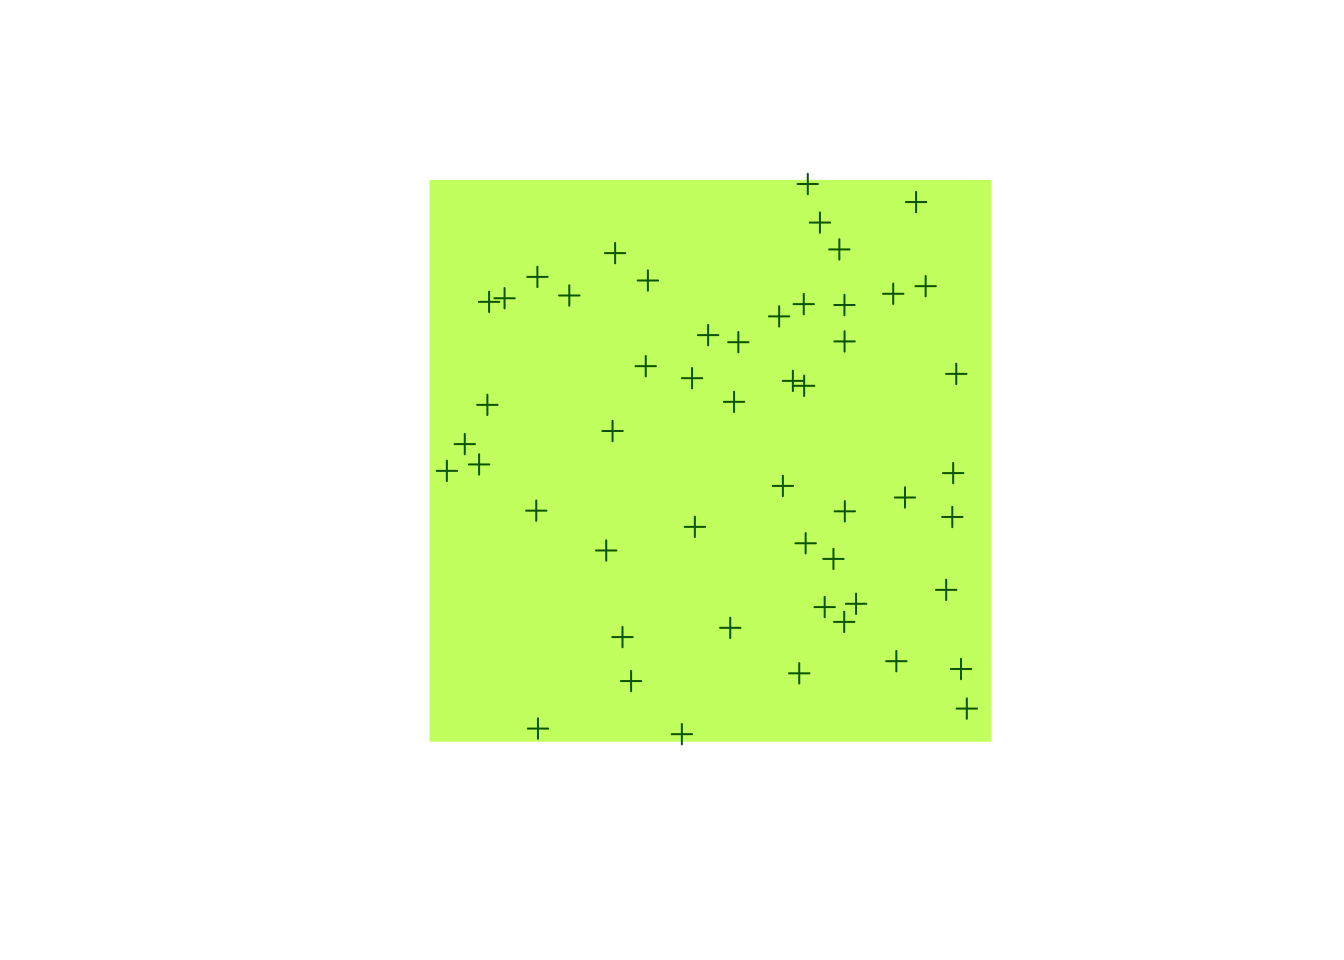
\includegraphics{qpad-book_files/figure-latex/unnamed-chunk-39-1.pdf}

\begin{Shaded}
\begin{Highlighting}[]
\NormalTok{mm <-}\StringTok{ }\KeywordTok{glm}\NormalTok{(y }\OperatorTok{~}\StringTok{ }\NormalTok{meth }\OperatorTok{-}\StringTok{ }\DecValTok{1}\NormalTok{, }\DataTypeTok{data=}\NormalTok{x, }\DataTypeTok{family=}\NormalTok{poisson)}
\KeywordTok{summary}\NormalTok{(mm)}
\end{Highlighting}
\end{Shaded}

\begin{verbatim}
## 
## Call:
## glm(formula = y ~ meth - 1, family = poisson, data = x)
## 
## Deviance Residuals: 
##    Min      1Q  Median      3Q     Max  
## -1.261  -1.261  -0.759   0.221   3.720  
## 
## Coefficients:
##       Estimate Std. Error z value            Pr(>|z|)    
## methA  -1.2444     0.0392  -31.77 <0.0000000000000002 ***
## methB  -0.2290     0.0234   -9.81 <0.0000000000000002 ***
## ---
## Signif. codes:  0 '***' 0.001 '**' 0.01 '*' 0.05 '.' 0.1 ' ' 1
## 
## (Dispersion parameter for poisson family taken to be 1)
## 
##     Null deviance: 7387.0  on 4569  degrees of freedom
## Residual deviance: 5683.8  on 4567  degrees of freedom
## AIC: 9171
## 
## Number of Fisher Scoring iterations: 6
\end{verbatim}

\begin{Shaded}
\begin{Highlighting}[]
\KeywordTok{exp}\NormalTok{(}\KeywordTok{coef}\NormalTok{(mm))}
\end{Highlighting}
\end{Shaded}

\begin{verbatim}
##  methA  methB 
## 0.2881 0.7953
\end{verbatim}

\begin{Shaded}
\begin{Highlighting}[]
\NormalTok{mm <-}\StringTok{ }\KeywordTok{glm}\NormalTok{(y }\OperatorTok{~}\StringTok{ }\NormalTok{Decid }\OperatorTok{+}\StringTok{ }\NormalTok{meth, }\DataTypeTok{data=}\NormalTok{x, }\DataTypeTok{family=}\NormalTok{poisson)}
\KeywordTok{summary}\NormalTok{(mm)}
\end{Highlighting}
\end{Shaded}

\begin{verbatim}
## 
## Call:
## glm(formula = y ~ Decid + meth, family = poisson, data = x)
## 
## Deviance Residuals: 
##    Min      1Q  Median      3Q     Max  
## -2.209  -0.855  -0.589   0.244   3.577  
## 
## Coefficients:
##             Estimate Std. Error z value            Pr(>|z|)    
## (Intercept)  -2.3275     0.0567   -41.0 <0.0000000000000002 ***
## Decid         2.1961     0.0689    31.9 <0.0000000000000002 ***
## methB         1.0284     0.0456    22.6 <0.0000000000000002 ***
## ---
## Signif. codes:  0 '***' 0.001 '**' 0.01 '*' 0.05 '.' 0.1 ' ' 1
## 
## (Dispersion parameter for poisson family taken to be 1)
## 
##     Null deviance: 6247.1  on 4568  degrees of freedom
## Residual deviance: 4595.6  on 4566  degrees of freedom
## AIC: 8085
## 
## Number of Fisher Scoring iterations: 6
\end{verbatim}

\begin{Shaded}
\begin{Highlighting}[]
\KeywordTok{boxplot}\NormalTok{(}\KeywordTok{fitted}\NormalTok{(mm) }\OperatorTok{~}\StringTok{ }\NormalTok{meth, x)}
\end{Highlighting}
\end{Shaded}

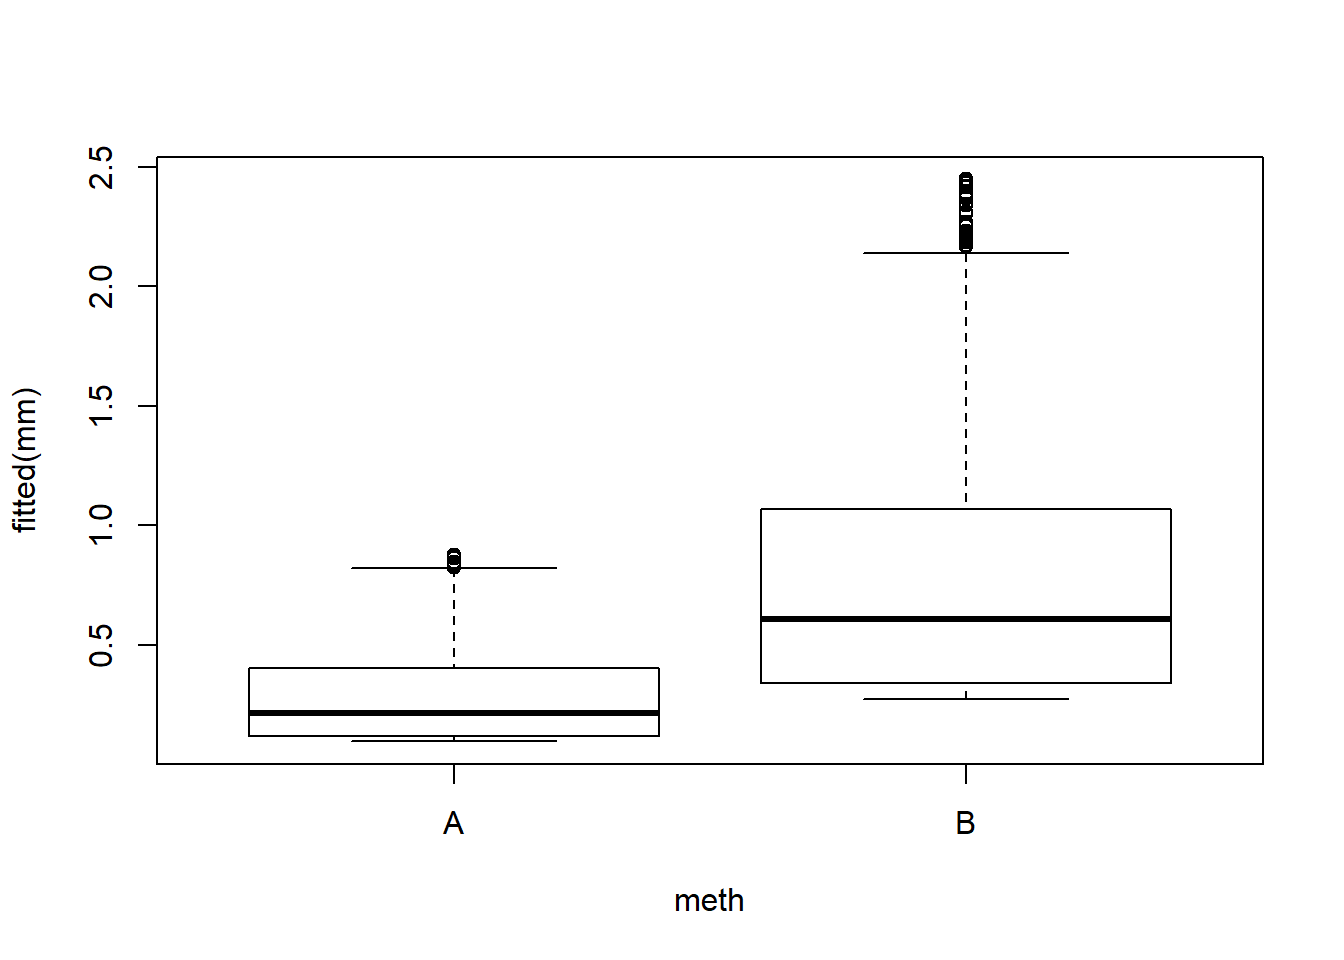
\includegraphics{qpad-book_files/figure-latex/unnamed-chunk-39-2.pdf}

\begin{Shaded}
\begin{Highlighting}[]
\KeywordTok{exp}\NormalTok{(}\KeywordTok{coef}\NormalTok{(mm))}
\end{Highlighting}
\end{Shaded}

\begin{verbatim}
## (Intercept)       Decid       methB 
##     0.09754     8.98996     2.79646
\end{verbatim}

\begin{Shaded}
\begin{Highlighting}[]
\KeywordTok{cumsum}\NormalTok{(}\KeywordTok{colMeans}\NormalTok{(y))[}\DecValTok{1}\OperatorTok{:}\DecValTok{2}\NormalTok{]}
\end{Highlighting}
\end{Shaded}

\begin{verbatim}
##   0-50m 50-100m 
##  0.2924  0.7846
\end{verbatim}

\begin{Shaded}
\begin{Highlighting}[]
\KeywordTok{mean}\NormalTok{(y[,}\DecValTok{1}\NormalTok{]) }\OperatorTok{*}\StringTok{ }\KeywordTok{c}\NormalTok{(}\DecValTok{1}\NormalTok{, }\KeywordTok{exp}\NormalTok{(}\KeywordTok{coef}\NormalTok{(mm))[}\DecValTok{3}\NormalTok{])}
\end{Highlighting}
\end{Shaded}

\begin{verbatim}
##         methB 
## 0.2924 0.8177
\end{verbatim}

\begin{Shaded}
\begin{Highlighting}[]
\NormalTok{mm <-}\StringTok{ }\KeywordTok{glm}\NormalTok{(y }\OperatorTok{~}\StringTok{ }\NormalTok{Decid, }\DataTypeTok{data=}\NormalTok{x, }\DataTypeTok{family=}\NormalTok{poisson,}
  \DataTypeTok{offset=}\KeywordTok{log}\NormalTok{(}\KeywordTok{ifelse}\NormalTok{(x}\OperatorTok{$}\NormalTok{meth }\OperatorTok{==}\StringTok{ "A"}\NormalTok{, }\FloatTok{0.5}\NormalTok{, }\DecValTok{1}\NormalTok{)}\OperatorTok{^}\DecValTok{2}\OperatorTok{*}\NormalTok{pi))}
\KeywordTok{summary}\NormalTok{(mm)}
\end{Highlighting}
\end{Shaded}

\begin{verbatim}
## 
## Call:
## glm(formula = y ~ Decid, family = poisson, data = x, offset = log(ifelse(x$meth == 
##     "A", 0.5, 1)^2 * pi))
## 
## Deviance Residuals: 
##    Min      1Q  Median      3Q     Max  
## -2.305  -0.842  -0.525   0.234   3.600  
## 
## Coefficients:
##             Estimate Std. Error z value            Pr(>|z|)    
## (Intercept)  -2.3658     0.0453   -52.2 <0.0000000000000002 ***
## Decid         2.2031     0.0690    31.9 <0.0000000000000002 ***
## ---
## Signif. codes:  0 '***' 0.001 '**' 0.01 '*' 0.05 '.' 0.1 ' ' 1
## 
## (Dispersion parameter for poisson family taken to be 1)
## 
##     Null deviance: 5746.0  on 4568  degrees of freedom
## Residual deviance: 4653.6  on 4567  degrees of freedom
## AIC: 8141
## 
## Number of Fisher Scoring iterations: 6
\end{verbatim}

\begin{Shaded}
\begin{Highlighting}[]
\KeywordTok{boxplot}\NormalTok{(}\KeywordTok{fitted}\NormalTok{(mm) }\OperatorTok{~}\StringTok{ }\NormalTok{meth, x)}
\end{Highlighting}
\end{Shaded}

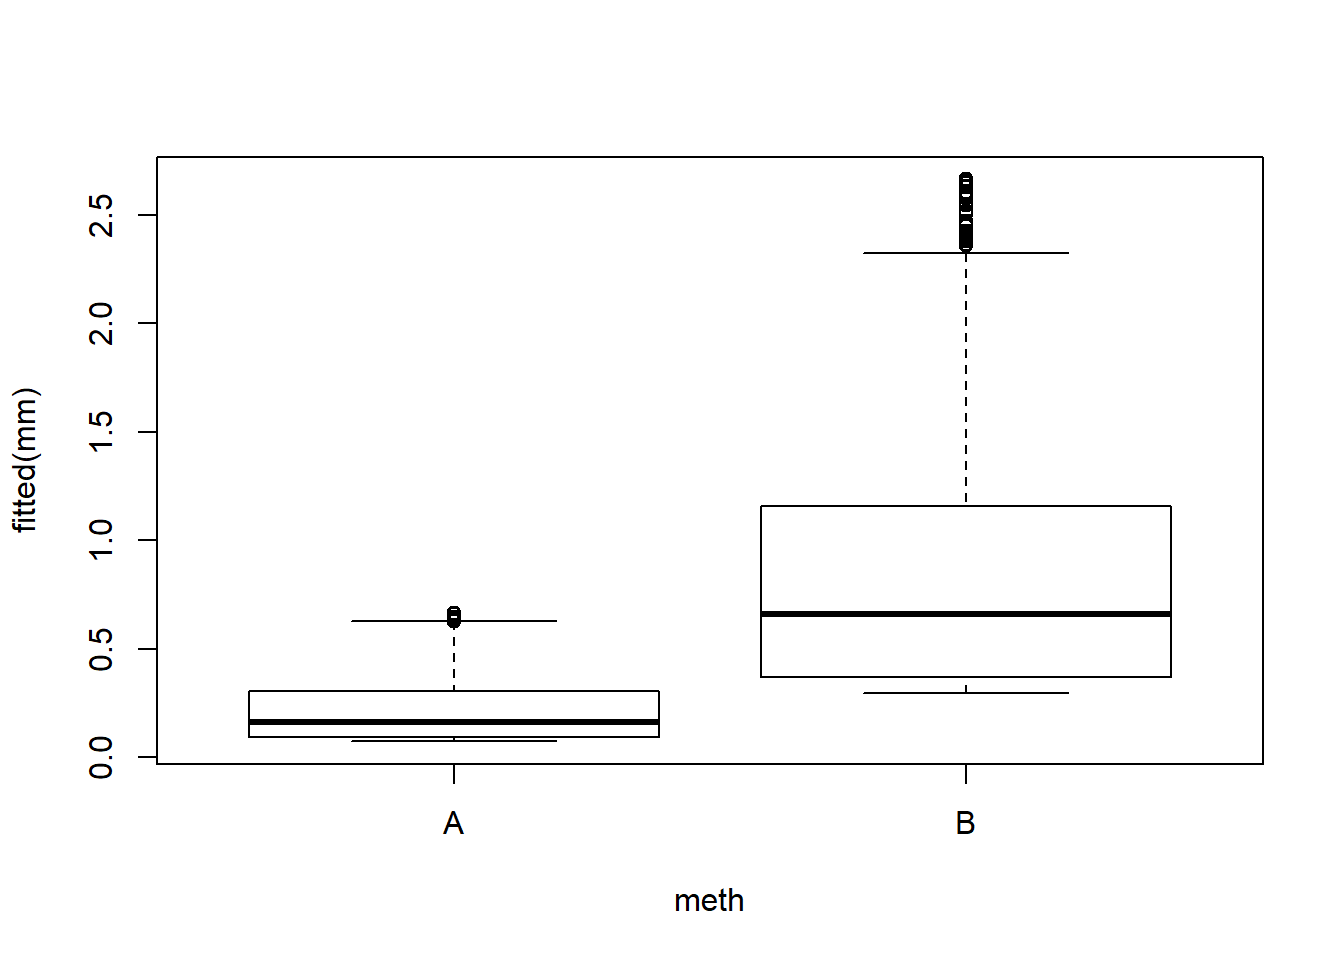
\includegraphics{qpad-book_files/figure-latex/unnamed-chunk-39-3.pdf}

\begin{Shaded}
\begin{Highlighting}[]
\KeywordTok{cumsum}\NormalTok{(}\KeywordTok{colMeans}\NormalTok{(y))[}\DecValTok{1}\OperatorTok{:}\DecValTok{2}\NormalTok{]}
\end{Highlighting}
\end{Shaded}

\begin{verbatim}
##   0-50m 50-100m 
##  0.2924  0.7846
\end{verbatim}

\begin{Shaded}
\begin{Highlighting}[]
\KeywordTok{c}\NormalTok{(}\FloatTok{0.5}\NormalTok{, }\DecValTok{1}\NormalTok{)}\OperatorTok{^}\DecValTok{2}\OperatorTok{*}\NormalTok{pi }\OperatorTok{*}\StringTok{ }\KeywordTok{mean}\NormalTok{(}\KeywordTok{exp}\NormalTok{(}\KeywordTok{model.matrix}\NormalTok{(mm) }\OperatorTok\StringTok{ }\KeywordTok{coef}\NormalTok{(mm))) }\CommentTok{# /ha}
\end{Highlighting}
\end{Shaded}

\begin{verbatim}
## [1] 0.2173 0.8691
\end{verbatim}

\hypertarget{definitions}{%
\section{Definitions}\label{definitions}}

Discuss definitions of:

\begin{itemize}
\tightlist
\item
  relative abundance,
\item
  abundance,
\item
  occupancy,
\item
  density.
\end{itemize}

\hypertarget{binomial-model-and-censoring}{%
\section{Binomial model and censoring}\label{binomial-model-and-censoring}}

Try cloglog with a rare species, like BOCH

\begin{Shaded}
\begin{Highlighting}[]
\CommentTok{#spp <- "OVEN" # which species}
\NormalTok{spp <-}\StringTok{ "BOCH"} \CommentTok{# which species}
\CommentTok{#spp <- "CAWA" # which species}

\NormalTok{x <-}\StringTok{ }\KeywordTok{data.frame}\NormalTok{(}
\NormalTok{  josm}\OperatorTok{$}\NormalTok{surveys, }
  \DataTypeTok{y=}\KeywordTok{as.numeric}\NormalTok{(ytot[}\KeywordTok{rownames}\NormalTok{(x), spp]))}
\NormalTok{x}\OperatorTok{$}\NormalTok{y01 <-}\StringTok{ }\KeywordTok{ifelse}\NormalTok{(x}\OperatorTok{$}\NormalTok{y }\OperatorTok{>}\StringTok{ }\DecValTok{0}\NormalTok{, }\DecValTok{1}\NormalTok{, }\DecValTok{0}\NormalTok{)}

\KeywordTok{table}\NormalTok{(x}\OperatorTok{$}\NormalTok{y)}
\end{Highlighting}
\end{Shaded}

\begin{verbatim}
## 
##    0    1    2    3 
## 4346  180   38    5
\end{verbatim}

\begin{Shaded}
\begin{Highlighting}[]
\NormalTok{mP <-}\StringTok{ }\KeywordTok{glm}\NormalTok{(y }\OperatorTok{~}\StringTok{ }\NormalTok{Decid }\OperatorTok{*}\StringTok{ }\NormalTok{ConifWet, x, }\DataTypeTok{family=}\NormalTok{poisson)}
\NormalTok{mBc <-}\StringTok{ }\KeywordTok{glm}\NormalTok{(y01 }\OperatorTok{~}\StringTok{ }\NormalTok{Decid }\OperatorTok{*}\StringTok{ }\NormalTok{ConifWet, x, }\DataTypeTok{family=}\KeywordTok{binomial}\NormalTok{(}\StringTok{"cloglog"}\NormalTok{))}
\NormalTok{mBl <-}\StringTok{ }\KeywordTok{glm}\NormalTok{(y01 }\OperatorTok{~}\StringTok{ }\NormalTok{Decid }\OperatorTok{*}\StringTok{ }\NormalTok{ConifWet, x, }\DataTypeTok{family=}\KeywordTok{binomial}\NormalTok{(}\StringTok{"logit"}\NormalTok{))}

\KeywordTok{coef}\NormalTok{(mP)}
\end{Highlighting}
\end{Shaded}

\begin{verbatim}
##    (Intercept)          Decid       ConifWet Decid:ConifWet 
##        -2.6836        -1.0105         0.2928         1.6797
\end{verbatim}

\begin{Shaded}
\begin{Highlighting}[]
\KeywordTok{coef}\NormalTok{(mBc)}
\end{Highlighting}
\end{Shaded}

\begin{verbatim}
##    (Intercept)          Decid       ConifWet Decid:ConifWet 
##        -2.8824        -0.9698         0.3459         1.6638
\end{verbatim}

\begin{Shaded}
\begin{Highlighting}[]
\KeywordTok{coef}\NormalTok{(mBl)}
\end{Highlighting}
\end{Shaded}

\begin{verbatim}
##    (Intercept)          Decid       ConifWet Decid:ConifWet 
##        -2.8550        -0.9889         0.3592         1.6844
\end{verbatim}

\begin{Shaded}
\begin{Highlighting}[]
\KeywordTok{plot}\NormalTok{(}\KeywordTok{fitted}\NormalTok{(mBc) }\OperatorTok{~}\StringTok{ }\KeywordTok{fitted}\NormalTok{(mP), }\DataTypeTok{col=}\DecValTok{4}\NormalTok{, }
  \DataTypeTok{ylim=}\KeywordTok{c}\NormalTok{(}\DecValTok{0}\NormalTok{, }\KeywordTok{max}\NormalTok{(}\KeywordTok{fitted}\NormalTok{(mP))), }\DataTypeTok{xlim=}\KeywordTok{c}\NormalTok{(}\DecValTok{0}\NormalTok{, }\KeywordTok{max}\NormalTok{(}\KeywordTok{fitted}\NormalTok{(mP))))}
\KeywordTok{points}\NormalTok{(}\KeywordTok{exp}\NormalTok{(}\KeywordTok{model.matrix}\NormalTok{(mBc) }\OperatorTok\StringTok{ }\KeywordTok{coef}\NormalTok{(mBc)) }\OperatorTok{~}\StringTok{ }\KeywordTok{fitted}\NormalTok{(mP), }\DataTypeTok{col=}\DecValTok{2}\NormalTok{)}
\KeywordTok{abline}\NormalTok{(}\DecValTok{0}\NormalTok{,}\DecValTok{1}\NormalTok{)}
\end{Highlighting}
\end{Shaded}

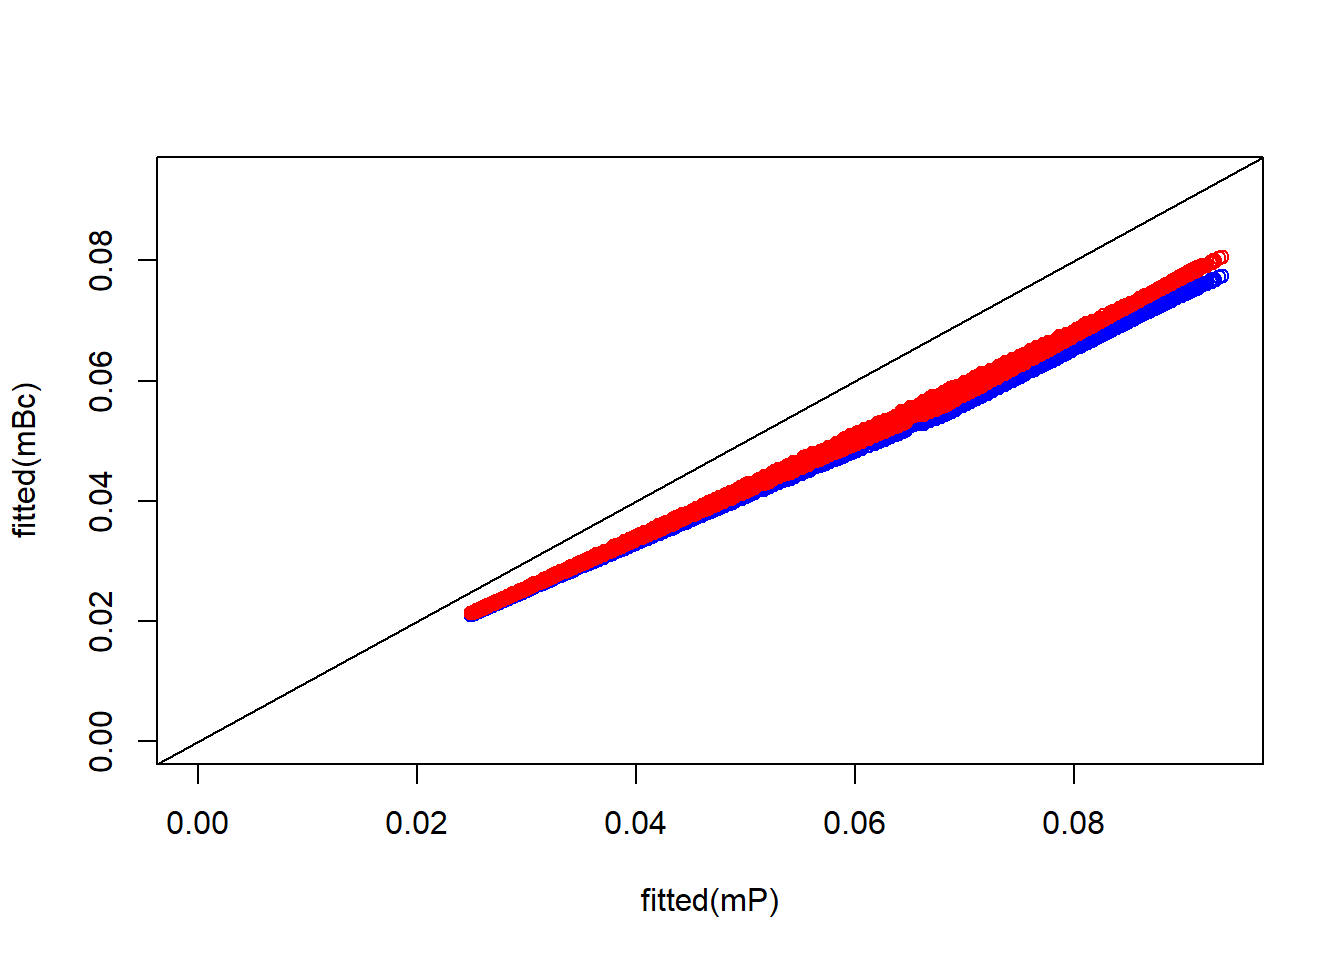
\includegraphics{qpad-book_files/figure-latex/unnamed-chunk-40-1.pdf}

\hypertarget{behavior}{%
\chapter{Behavioral Complexities}\label{behavior}}

Behaviour related stuff

constant p (time as covariate)

time varying p

finite mix

time varying p/c

rate, count, time-to-event

\hypertarget{detection}{%
\chapter{The Detection Process}\label{detection}}

EDR, tau constant

truncated, unlimited

variable tau: habitat effect (continuous case?)

discrete: land cover, observer effects

contrast fixed effects with offsets -- motivation for ARU

\hypertarget{recordings}{%
\chapter{Dealing with Recordings}\label{recordings}}

integration challenges

calibration (exponential/cloglog approximation)

fixed effects

paired

sensor sensitivity - EDR

\hypertarget{assumptions}{%
\chapter{A Closer Look at Assumptions}\label{assumptions}}

break thos assumptions

\hypertarget{roadsides}{%
\chapter{Understanding Roadside Surveys}\label{roadsides}}

directional diff in signal transmission

\hypertarget{extras}{%
\chapter{Miscellaneous Topics}\label{extras}}

model selection and conditional likelihood

variance/bias trade off

error propagation

MCMC?

N-mixture ideas

phylogenetic and life history/trait stuff

PIF methods

\bibliography{book.bib,packages.bib}


\end{document}
